% ============================================================================
%  Algoritmos del núcleo de Tukit
%  Documento principal: reúne el preámbulo y las secciones de `secciones/`.
%  Compilar desde esta carpeta:  latexmk -pdf main.tex   (o pdflatex x2)
% ============================================================================
\documentclass[11pt,letterpaper]{article}

% ============================================================================
%  Preámbulo
% ============================================================================

% ---- Idioma y tipografía ---------------------------------------------------
\usepackage[T1]{fontenc}
\usepackage[utf8]{inputenc}
\usepackage[spanish,es-noshorthands,es-tabla,es-nodecimaldot]{babel}
\usepackage{lmodern}
\usepackage{microtype}
\usepackage{csquotes}

% ---- Página ----------------------------------------------------------------
\usepackage[margin=2.6cm,headheight=14pt]{geometry}
\usepackage{fancyhdr}
\pagestyle{fancy}
\fancyhf{}
\fancyhead[L]{\small\nouppercase{\leftmark}}
\fancyhead[R]{\small Algoritmos del núcleo de Tukit}
\fancyfoot[C]{\small\thepage}
\renewcommand{\headrulewidth}{0.4pt}
\setlength{\parskip}{0.35em}

% ---- Matemáticas -----------------------------------------------------------
\usepackage{amsmath,amssymb,amsthm,mathtools}
\usepackage{siunitx}
\sisetup{output-decimal-marker={,}, group-separator={.}, group-minimum-digits=4}

% ---- Tablas, figuras, listas ----------------------------------------------
\usepackage{booktabs,multirow,threeparttable,array}
\newcolumntype{L}[1]{>{\raggedright\arraybackslash}p{#1}}
\usepackage{graphicx}
\usepackage{float}
\usepackage[font=small,labelfont=bf]{caption}
\usepackage[inline]{enumitem}
\setlist{itemsep=0.15em,topsep=0.3em}

% ---- Pseudocódigo ----------------------------------------------------------
\usepackage{algorithm}
\usepackage[noend]{algpseudocode}
\floatname{algorithm}{Algoritmo}
\renewcommand{\listalgorithmname}{Lista de algoritmos}
\algrenewcommand\algorithmicrequire{\textbf{Entrada:}}
\algrenewcommand\algorithmicensure{\textbf{Salida:}}
\algrenewcommand\algorithmicif{\textbf{si}}
\algrenewcommand\algorithmicthen{\textbf{entonces}}
\algrenewcommand\algorithmicelse{\textbf{si no}}
\algrenewcommand\algorithmicfor{\textbf{para}}
\algrenewcommand\algorithmicforall{\textbf{para todo}}
\algrenewcommand\algorithmicdo{\textbf{hacer}}
\algrenewcommand\algorithmicwhile{\textbf{mientras}}
\algrenewcommand\algorithmicreturn{\textbf{devolver}}
\algrenewcommand\algorithmicfunction{\textbf{función}}
\algrenewcommand\algorithmicprocedure{\textbf{procedimiento}}
\algrenewcommand\algorithmicrepeat{\textbf{repetir}}
\algrenewcommand\algorithmicuntil{\textbf{hasta}}
\algnewcommand\algorithmicand{\textbf{y}}
\algnewcommand\algorithmicor{\textbf{o}}
\algnewcommand\AND{\algorithmicand}
\algnewcommand\OR{\algorithmicor}
\algnewcommand{\LineComment}[1]{\State \(\triangleright\) \textit{#1}}
\algrenewcommand\alglinenumber[1]{\scriptsize #1:}

% ---- Diagramas y gráficas -------------------------------------------------
\usepackage{tikz}
\usetikzlibrary{arrows.meta,positioning,shapes.geometric,fit,calc,backgrounds}
\usepackage{pgfplots}
\pgfplotsset{compat=1.18}
\usepgfplotslibrary{groupplots}

% ---- Colores y bloques (en la línea de las notas de clase) ----------------
\usepackage{xcolor}
\definecolor{azul}{RGB}{40,40,150}
\definecolor{azulclaro}{RGB}{232,232,246}
\definecolor{verde}{RGB}{20,110,40}
\definecolor{verdeclaro}{RGB}{230,243,232}
\definecolor{rojo}{RGB}{170,40,40}
\definecolor{rojoclaro}{RGB}{248,232,232}
\definecolor{gris}{RGB}{90,90,90}
\definecolor{grisclaro}{RGB}{242,242,242}

\usepackage[most]{tcolorbox}
\tcbset{
  bloque/.style={enhanced, breakable, arc=1.5mm, boxrule=0.6pt,
    left=2mm, right=2mm, top=1mm, bottom=1mm,
    fonttitle=\bfseries\small, coltitle=white},
}

% Caja para registrar la evolución de un algoritmo: antes / defecto / cambio.
\newtcolorbox{evolucion}[1][]{bloque, colback=grisclaro, colframe=gris,
  title={Evolución#1}}
% Caja de advertencia o de hallazgo crítico (el título es obligatorio).
\newtcolorbox{hallazgo}[1]{bloque, colback=rojoclaro, colframe=rojo,
  title={#1}}

% ---- Referencias cruzadas --------------------------------------------------
\usepackage{xurl}
\usepackage[hidelinks,pdfusetitle,bookmarksnumbered]{hyperref}
\usepackage[spanish,nameinlink,noabbrev]{cleveref}

% Teoremas con numeración por sección. Se definen DESPUÉS de cleveref para que
% \cref distinga entornos que comparten contador (teorema, proposición, ...).
% Cada entorno tiene un contador alias del de `definicion`: comparten la
% numeración, pero cleveref sabe cómo llamar a cada uno.
\usepackage{aliascnt}
\newcommand{\nuevoenunciado}[2]{%
  \newaliascnt{#1}{definicion}%
  \newtheorem{#1}[#1]{#2}%
  \aliascntresetthe{#1}}
\theoremstyle{definition}
\newtheorem{definicion}{Definición}[section]
\nuevoenunciado{ejemplo}{Ejemplo}
\nuevoenunciado{observacion}{Observación}
\theoremstyle{plain}
\nuevoenunciado{proposicion}{Proposición}
\nuevoenunciado{lema}{Lema}
\nuevoenunciado{teorema}{Teorema}
\nuevoenunciado{corolario}{Corolario}
\renewcommand{\qedsymbol}{$\blacksquare$}

% Cajas de color alrededor de los enunciados principales.
\tcolorboxenvironment{definicion}{bloque, colback=azulclaro, colframe=azul}
\tcolorboxenvironment{proposicion}{bloque, colback=verdeclaro, colframe=verde}
\tcolorboxenvironment{teorema}{bloque, colback=verdeclaro, colframe=verde}
\tcolorboxenvironment{lema}{bloque, colback=verdeclaro, colframe=verde}
\crefname{section}{sección}{secciones}
\crefname{subsection}{sección}{secciones}
\crefname{subsubsection}{sección}{secciones}
\crefname{appendix}{apéndice}{apéndices}
\crefname{table}{tabla}{tablas}
\crefname{figure}{figura}{figuras}
\crefname{equation}{ecuación}{ecuaciones}
\crefname{enumi}{requisito}{requisitos}
\crefname{definicion}{definición}{definiciones}
\crefname{proposicion}{proposición}{proposiciones}
\crefname{lema}{lema}{lemas}
\crefname{teorema}{teorema}{teoremas}
\crefname{corolario}{corolario}{corolarios}
\crefname{observacion}{observación}{observaciones}
\crefname{ejemplo}{ejemplo}{ejemplos}
\crefname{algorithm}{algoritmo}{algoritmos}
\crefname{ALG@line}{línea}{líneas}

% ---- Notación ----------------------------------------------------------------
\newcommand{\N}{\mathbb{N}}
\newcommand{\R}{\mathbb{R}}
\newcommand{\Z}{\mathbb{Z}}
\newcommand{\Cat}{\mathcal{C}}          % conceptos
\newcommand{\Prod}{\mathcal{P}}         % productos
\newcommand{\Tipos}{\mathcal{T}}        % tipos de renglón
\newcommand{\Est}{\mathcal{E}}          % estados de resolución
\newcommand{\Dec}{\mathcal{D}}          % líneas decidibles
\newcommand{\Esp}{\Omega}               % espacio de búsqueda
\newcommand{\Front}{\mathcal{F}}        % frente
\newcommand{\nivel}{\nu}
\newcommand{\precio}{\pi}
\newcommand{\emp}{\upsilon}             % unidades por empaque
\newcommand{\techo}[1]{\left\lceil #1 \right\rceil}
\newcommand{\piso}[1]{\left\lfloor #1 \right\rfloor}
\newcommand{\abs}[1]{\left\lvert #1 \right\rvert}
\newcommand{\card}[1]{\left\lvert #1 \right\rvert}
\newcommand{\ind}[1]{\mathbf{1}\!\left[#1\right]}
\newcommand{\domina}{\prec}
\newcommand{\sinprecio}{\bot}
\newcommand{\cod}[1]{\texttt{#1}}
\DeclareMathOperator*{\argmin}{arg\,min}
\DeclareMathOperator*{\argmax}{arg\,max}
\DeclareMathOperator*{\lexmin}{lex\,min}
\DeclareMathOperator*{\lexmax}{lex\,max}
\DeclareMathOperator{\sing}{sing}
\DeclareMathOperator{\cab}{cab}
\DeclareMathOperator{\sig}{sig}


% ---------------------------------------------------------------- Portada ----
% Los campos marcados como pendientes se completan después.
\newcommand{\Autor}{Gabriel Riaño}
\newcommand{\Universidad}{Pontificia Universidad Javeriana}
\newcommand{\Facultad}{[Facultad — pendiente]}
\newcommand{\Departamento}{[Departamento — pendiente]}
\newcommand{\Programa}{[Programa — pendiente]}
\newcommand{\Director}{[Director(a) — pendiente]}
\newcommand{\Lugar}{[Ciudad — pendiente]}
\newcommand{\Fecha}{[Fecha — pendiente]}

\title{%
  \textbf{Algoritmos del núcleo de Tukit}\\[0.4em]
  \large Percepción de listas escolares, resolución híbrida contra un catálogo\\
  curado y optimización multiobjetivo de kits}
\author{\Autor\\[0.3em]
  \small \Universidad\\
  \small \Facultad\ \textperiodcentered\ \Departamento\\
  \small \Programa\\[0.3em]
  \small Director(a): \Director}
\date{\Lugar, \Fecha}

\begin{document}

\maketitle
\thispagestyle{empty}

\begin{abstract}
\noindent
Tukit recibe la lista de útiles que un colegio entrega a las familias y devuelve
kits de compra que equilibran precio, calidad de marca, disponibilidad y la
preferencia por personajes. Este documento describe con rigor formal los
algoritmos que hacen ese recorrido, en el orden en que se ejecutan:
\begin{enumerate*}[label=(\roman*)]
  \item la \emph{percepción}, que convierte un archivo en renglones o lo rechaza
        completo;
  \item la \emph{normalización}, que separa qué se pide de cuánto se pide;
  \item la \emph{resolución}, que asigna cada renglón a un concepto del
        catálogo mediante una función de puntaje léxico-semántica con abstención;
  \item el \emph{mantenimiento del catálogo}, que garantiza las propiedades que
        las etapas anteriores suponen; y
  \item la \emph{optimización}, que construye un frente de Pareto de cuatro
        objetivos ---por enumeración exacta o con NSGA-II--- y lo proyecta en
        los kits que se ofrecen y en uno recomendado.
\end{enumerate*}
Para cada algoritmo se da la definición del problema, la formulación, el
pseudocódigo, el análisis de complejidad, las propiedades que se pueden
demostrar y la evolución que tuvo durante el proyecto, con las mediciones que la
motivaron. El documento incluye también un análisis estructural del problema
de optimización que muestra que, con la formulación vigente, el frente exacto
se puede calcular en tiempo polinomial, y discute lo que eso implica.
\end{abstract}

\vspace{1em}
\noindent\textbf{Palabras clave:} optimización multiobjetivo, NSGA-II, frente
de Pareto, mochila de elección múltiple, distancia de edición, similitud de
Jaccard, \emph{embeddings}, búsqueda híbrida, modelos multimodales.

\clearpage
\tableofcontents
\clearpage

% ============================================================================
\section{Introducción}
\label{sec:intro}
% ============================================================================

Cada año los colegios entregan a las familias una lista de útiles: un documento
escrito por materias, con redacciones libres, cantidades que a veces están en
una columna y a veces dentro del texto, marcas sugeridas, instrucciones del
tipo «el disponible en casa» y libros de edición cerrada. Convertir ese
documento en una compra exige resolver tres problemas de naturaleza distinta,
que se encadenan:

\begin{enumerate}
  \item \textbf{Leer.} Pasar de un archivo (PDF o imagen), cuya estructura es
        visual ---tablas, columnas, filas que ocupan dos líneas---, a una
        secuencia de renglones, cada uno con su descripción y su cantidad.
        Además hay que decidir si el archivo corresponde a la lista de
        \emph{un} grado.
  \item \textbf{Entender.} Decidir qué pide cada renglón en términos de un
        catálogo propio y curado: a qué \emph{concepto} corresponde
        («cuaderno», «témpera», «juego de geometría»), qué atributos exige
        («tamaño oficio», «cuadriculado») y si el catálogo puede cumplirlo.
        Si no puede, hay que decirlo en lugar de ofrecer otra cosa.
  \item \textbf{Elegir.} Para cada renglón que se puede comprar hay varios
        productos admisibles, con precios, niveles de marca, empaques y
        personajes distintos. El conjunto de elecciones forma un \emph{kit}, y
        lo que una familia valora de un kit es un compromiso entre objetivos
        en conflicto: precio, calidad de marca, disponibilidad y, a veces, el
        personaje favorito de un hijo.
\end{enumerate}

Este documento describe los algoritmos con los que el sistema resuelve los
tres problemas. Cubre únicamente el \emph{núcleo algorítmico} y deja por fuera
los mecanismos de plataforma (pagos, colas de trabajo, identidad, despliegue).
El objetivo es que un lector con formación en análisis de algoritmos pueda
reconstruir cada decisión a partir de la definición formal del problema, y
juzgar si es correcta y cuánto cuesta.

\subsection{Contribuciones del documento}

\begin{itemize}
  \item Un \textbf{modelo formal único} (\cref{sec:modelo}) que fija la
        notación de todas las etapas y define el sistema como una composición
        de funciones con estados de error explícitos.
  \item Para cada etapa, la \textbf{definición del problema}, el
        \textbf{pseudocódigo}, el \textbf{análisis de complejidad} y las
        \textbf{propiedades demostrables} que la implementación cumple
        ---por ejemplo, que la percepción nunca devuelve una lista truncada, que
        la fusión léxico-semántica nunca puntúa por debajo del canal léxico o
        que consolidar la compra entre hermanos nunca aumenta el costo.
  \item Un \textbf{análisis estructural del problema de optimización}
        (\cref{sec:opt-estructura}). Bajo la formulación vigente, los cuatro
        objetivos son aditivos por línea, los extremos del frente se resuelven
        de forma voraz y exacta, y el frente completo se puede calcular en
        tiempo polinomial mediante programación dinámica. Este resultado
        explica por qué el NSGA-II iguala al óptimo en los extremos y por qué
        su aporte real está en el compromiso con presupuesto.
  \item Una \textbf{evaluación empírica} sobre 174 listas oficiales reales
        (\cref{sec:evaluacion}), con un óptimo exacto como referencia y líneas
        base que incluyen un modelo de decisión de propósito general.
  \item Un \textbf{registro de la evolución} de cada algoritmo
        (\cref{sec:evolucion} y los recuadros «Evolución» de cada sección):
        qué versión existió, qué defecto medido la hizo cambiar y qué efecto
        tuvo el cambio.
\end{itemize}

\subsection{Principios de diseño transversales}
\label{sec:principios}

Algunas decisiones se repiten en todas las etapas. Conviene enunciarlas antes
porque explican la forma de los algoritmos, y no solo su contenido.

\begin{description}[style=nextline]
  \item[Abstenerse es una respuesta válida.] En todas las etapas existe una
        salida que significa «no lo sé» o «no lo tengo», y se prefiere a una
        respuesta plausible pero incorrecta. La percepción rechaza el archivo
        completo antes que entregar una lista a medias. El emparejador se
        abstiene si ningún producto declara el atributo que el colegio exige.
        La corrección ortográfica solo corrige cuando hay \emph{una} candidata.
        La razón es la asimetría de costos: un kit incompleto que se presenta
        como completo, o un producto equivocado en el carrito, solo lo descubre
        la familia cuando recibe el pedido.
  \item[Separar decidir de presentar.] La aritmética de unidades, las líneas
        informativas que no se cobran y la consolidación son independientes del
        algoritmo que selecciona productos. Así el optimizador se puede
        reemplazar sin tocar lo que el acudiente ve.
  \item[Determinismo y reproducibilidad.] Con la misma entrada y la misma
        semilla, el resultado es idéntico byte a byte: los empates se rompen por
        claves totales (por ejemplo, el SKU) y el NSGA-II termina por número de
        generaciones y no por convergencia.
  \item[Lo curado manda sobre lo inferido.] Cuando un dato revisado por una
        persona está disponible (el concepto asignado a un renglón, el tipo de
        renglón declarado en la lista oficial), se usa en lugar de volver a
        inferirlo del texto.
  \item[Degradar en lugar de fallar, pero nunca en silencio.] Si el canal
        semántico no está disponible, la resolución continúa solo con el canal
        léxico y lo registra. Si la percepción no puede leer una página, el
        trabajo falla con un diagnóstico y se puede reintentar. No se
        fabrica una respuesta.
\end{description}

\subsection{Organización}

La \cref{sec:modelo} establece el modelo y la notación. Las
\cref{sec:percepcion,sec:normalizacion,sec:resolucion} siguen el flujo de
datos: percepción, normalización y resolución. La \cref{sec:catalogo} describe
los algoritmos que mantienen las propiedades del catálogo de las que dependen la
resolución y la optimización. La \cref{sec:optimizacion}, la más extensa,
desarrolla la optimización multiobjetivo. La \cref{sec:evaluacion} presenta la
evaluación empírica, la \cref{sec:evolucion} consolida la evolución y la
\cref{sec:discusion} discute limitaciones y trabajo futuro. Los apéndices
reúnen todos los parámetros numéricos con su justificación y la correspondencia
entre cada algoritmo y el módulo que lo implementa.

% ============================================================================
\section{Modelo formal y notación}
\label{sec:modelo}
% ============================================================================

Esta sección fija los objetos sobre los que operan todos los algoritmos. Las
secciones siguientes usan esta notación sin volver a definirla.

\subsection{El catálogo}

\begin{definicion}[Concepto]
\label{def:concepto}
Un \emph{concepto} es una clase de productos intercambiables desde el punto de
vista del colegio: si la lista pide un elemento del concepto, cualquier otro
elemento del mismo concepto la satisface, salvo por los atributos que el
renglón exija. Formalmente, un concepto es una tupla
\[
  c = \bigl(\mathrm{cod}(c),\ \mathrm{nom}(c),\ S(c),\ D(c),\ t(c)\bigr),
\]
donde $\mathrm{cod}(c)$ es un código estable (por ejemplo \cod{C001}),
$\mathrm{nom}(c)$ el nombre canónico, $S(c)$ un conjunto finito de sinónimos
(frases con las que los colegios nombran el concepto), $D(c)$ el conjunto de
\emph{atributos discriminantes} (los que filtran productos, como
\cod{tamano} o \cod{rayado}) y $t(c)\in\Tipos$ el tipo de renglón que el
concepto representa. $\Cat$ denota el conjunto de conceptos activos.
\end{definicion}

El criterio para separar dos conceptos es operativo: se crea un concepto
distinto solo cuando reemplazar uno por el otro \emph{no} satisface al colegio.
Por ejemplo, la cartulina iris no reemplaza al papel iris porque su gramaje es
distinto. En cambio, el cuaderno cuadriculado y el de cinco materias son el
mismo concepto con atributos distintos.

\begin{definicion}[Producto canónico]
\label{def:producto}
Un \emph{producto} es una tupla
\[
  p = \bigl(\mathrm{sku}(p),\ c(p),\ \nivel(p),\ \precio(p),\ \emp(p),\
           \mathrm{per}(p),\ \alpha(p)\bigr),
\]
donde $c(p)\in\Cat$ es su concepto, $\nivel(p)\in\{0,1,2\}$ su nivel de marca
(económico, confiable, premium), $\precio(p)\in\N\cup\{\sinprecio\}$ el menor
precio vigente entre sus ofertas en tiendas, con $\sinprecio$ cuando no hay
ninguno, $\emp(p)\in\N_{\geq 1}$ las unidades por empaque,
$\mathrm{per}(p)$ el personaje que trae (o ninguno) y
$\alpha(p)\colon \mathrm{Atr}\rightharpoonup \mathrm{Val}$ una función parcial
de atributos declarados. $\Prod$ denota el conjunto de productos activos y
$\Prod(c)=\{p\in\Prod : c(p)=c\}$.
\end{definicion}

\begin{observacion}[Nivel frente a perfil]
El nivel $\nivel(p)$ describe un \emph{producto}. Los perfiles de kit
(Ahorrador, Premium, Fan, A~tu~Medida) describen una \emph{preferencia sobre
el kit completo}. Son ejes distintos aunque compartan la palabra «premium»: un
kit Ahorrador puede contener un producto de nivel premium si resulta el más
barato una vez se tiene en cuenta el empaque.
\end{observacion}

\subsection{Renglones, tipos y modos}

\begin{definicion}[Tipos y modos]
\label{def:tipos}
El conjunto de \emph{tipos de renglón} es
\begin{align*}
  \Tipos = \{&\cod{util},\ \cod{libro\_libre},\ \cod{texto},\ \cod{licencia\_digital},\\
             &\cod{no\_comprar},\ \cod{diferido},\ \cod{uniforme},\ \cod{otro}\},
\end{align*}
y el de \emph{modos de adquisición}
\begin{align*}
  \mathcal{M} = \{&\cod{mercado\_abierto},\ \cod{libro\_libre},\ \cod{venta\_directa\_editorial},\\
                  &\cod{edicion\_exclusiva},\ \cod{plataforma},\ \cod{diferido}\}.
\end{align*}
Se distinguen los tipos \emph{buscables} $\Tipos_b=\{\cod{util},
\cod{libro\_libre}\}$ y los modos \emph{surtibles}
$\mathcal{M}_s=\{\cod{mercado\_abierto},\cod{libro\_libre}\}$.
\end{definicion}

\begin{definicion}[Renglón y demanda]
\label{def:renglon}
Un \emph{renglón crudo} es un par $\rho=(x,q^\circ)$ con $x\in\Sigma^*$ su
texto y $q^\circ\in\N\cup\{\varnothing\}$ la cantidad leída en una columna, si
existía. La normalización (\cref{sec:normalizacion}) lo convierte en una
\emph{demanda}
\[
  r = \bigl(x,\ t(r),\ m(r),\ q(r),\ \emp^{\mathrm{txt}}(r)\bigr),
\]
con $t(r)\in\Tipos$, $m(r)\in\mathcal{M}$, $q(r)\in\N$ la cantidad pedida en
unidades base y $\emp^{\mathrm{txt}}(r)$ el empaque que el propio texto
declara, si lo hace. Un renglón \emph{se busca en el catálogo} si y solo si
$t(r)\in\Tipos_b \wedge m(r)\in\mathcal{M}_s$, y es \emph{informativo} si y
solo si $t(r)\notin\Tipos_b' \vee m(r)\notin\mathcal{M}_s$, donde
$\Tipos_b'=\Tipos\setminus\{\cod{licencia\_digital},\cod{no\_comprar},
\cod{diferido},\cod{uniforme},\cod{otro}\}$. Un renglón informativo se
muestra al acudiente con su instrucción y \emph{nunca} se cobra.
\end{definicion}

Los dos predicados no coinciden: un renglón de tipo \cod{texto} en
\cod{mercado\_abierto} no se busca en el catálogo de útiles, porque su
respuesta es una edición concreta y no un parecido, pero tampoco es
informativo, porque es papel que se puede comprar.

\subsection{Resolución y estados}

\begin{definicion}[Estados de resolución]
\label{def:estados}
El resultado de resolver un renglón contra el catálogo toma un valor en
\[
  \Est = \{\textsc{ResueltoAuto},\ \textsc{Ambiguo},\ \textsc{SinMatch},\
          \textsc{HuecoCatálogo}\}.
\]
\textsc{SinMatch} significa «no entendí qué se pide»; \textsc{HuecoCatálogo}
significa «entendí qué se pide y el catálogo no lo tiene» (o no tiene un
producto con el atributo exigido). La distinción importa porque solo el
segundo se puede atender con una alternativa o con una disculpa útil.
\textsc{Ambiguo} significa que el sistema tiene una hipótesis, pero su
confianza está por debajo del umbral $\tau$ y una persona debe confirmarla.
\end{definicion}

\subsection{Hogar, preferencias y kit}

Una solicitud se hace \emph{por hogar} y no por hijo. Un hogar $H$ es un
conjunto de hijos $h$, cada uno con su colegio y su grado, y por lo tanto con
su lista. Las preferencias del acudiente son una tupla con: prioridad
(\emph{lo más económico}, \emph{equilibrio}, \emph{puedo estirarme}), pesos
declarados, disposición a pagar sobreprecio $\sigma\in[0,1]$, un tope de gasto
opcional $B$ y, para cada hijo, un conjunto opcional de personajes pedidos
$\Pi_h$.

\begin{definicion}[Kit]
\label{def:kit}
Sea $R$ la secuencia de demandas de todos los hijos del hogar. Un \emph{kit}
es una asignación $k\colon R\to\Prod\cup\{\varnothing\}$ que a cada renglón
buscable le asigna un producto admisible (o ninguno si no hay) y a cada
renglón informativo le asigna $\varnothing$, junto con la aritmética derivada:
unidades a comprar, subtotales y total. Un kit lleva un \emph{perfil}, que es
la regla que lo eligió.
\end{definicion}

\subsection{El sistema como composición}

El sistema se puede escribir como una composición de funciones parciales, en
la que cada etapa puede terminar en un estado de rechazo explícito:
\begin{multline*}
  \underbrace{\text{archivo}}_{\text{PDF / imagen}}
  \xrightarrow{\ \Phi_{\mathrm{per}}\ }
  \underbrace{(\rho_1,\dots,\rho_m)}_{\text{renglones}}
  \xrightarrow{\ \text{revisión}\ }
  \text{lista oficial}\\
  \xrightarrow{\ \Phi_{\mathrm{nor}}\ }
  (r_1,\dots,r_m)
  \xrightarrow{\ \Phi_{\mathrm{res}}\ }
  (r_i, e_i, A_i)_{i}
  \xrightarrow{\ \Phi_{\mathrm{opt}}\ }
  (k_{\text{Ah}}, k_{\text{Pr}}, \dots;\ k^\star)
\end{multline*}
donde $e_i\in\Est$ es el estado de resolución, $A_i$ el conjunto de candidatos
admisibles del renglón $i$ y $k^\star$ el kit recomendado. La
\cref{fig:pipeline} muestra el flujo con las dos rutas que existen en la
práctica.

\begin{figure}[htbp]
\centering
\begin{tikzpicture}[
  node distance=6mm and 9mm,
  etapa/.style={draw=azul, fill=azulclaro, rounded corners=2pt, align=center,
                minimum height=10mm, text width=25mm, font=\small},
  dato/.style={draw=gris, fill=grisclaro, align=center, font=\footnotesize,
               text width=22mm, minimum height=8mm},
  humano/.style={draw=verde, fill=verdeclaro, rounded corners=2pt, align=center,
                 font=\small, text width=25mm, minimum height=10mm},
  rechazo/.style={draw=rojo, fill=rojoclaro, align=center, font=\footnotesize,
                  text width=40mm},
  flecha/.style={-{Stealth[length=2.2mm]}, thick},
]
\node[dato] (pdf) {Archivo\\(PDF o imagen)};
\node[etapa, right=of pdf] (per) {\textbf{Percepción}\\\cref{sec:percepcion}};
\node[humano, right=of per] (rev) {Revisión humana de la lista};
\node[dato, right=of rev] (lista) {Lista oficial revisada};
\node[rechazo, above=of per] (rech) {Rechazo completo\\(varios grados, página incompleta, \dots)};

\node[etapa, below=16mm of lista] (nor) {\textbf{Normalización}\\\cref{sec:normalizacion}};
\node[etapa, left=of nor] (res) {\textbf{Resolución}\\\cref{sec:resolucion}};
\node[etapa, left=of res] (opt) {\textbf{Optimización}\\\cref{sec:optimizacion}};
\node[dato, left=of opt] (kits) {Kits y recomendado};
\node[humano, below=of res] (hitl) {Revisión de líneas \textsc{Ambiguo}};
\node[dato, below=of nor, text width=27mm] (cat) {Catálogo curado $(\Cat,\Prod)$\\\cref{sec:catalogo}};

\draw[flecha] (pdf) -- (per);
\draw[flecha] (per) -- (rev);
\draw[flecha] (rev) -- (lista);
\draw[flecha, rojo] (per) -- (rech);
\draw[flecha] (lista) -- (nor);
\draw[flecha] (nor) -- (res);
\draw[flecha] (res) -- (opt);
\draw[flecha] (opt) -- (kits);
\draw[flecha, dashed] (res) -- (hitl);
\draw[flecha, dashed] (cat) -- (res);
\draw[flecha, verde, dashed, rounded corners]
  (lista.east) -- ++(5mm,0) |- ($(hitl.south)+(0,-5mm)$) -| (opt.south)
  node[pos=0.25, below, font=\footnotesize] {ruta rápida: el concepto ya está asignado};
\end{tikzpicture}
\caption{Flujo del núcleo. La percepción ocurre cuando se sube el archivo y
alimenta una revisión humana de la lista. Una vez revisada, la lista se
reutiliza para todas las familias del mismo colegio y grado. La ruta rápida
(verde) evita volver a percibir y a resolver una lista ya revisada.}
\label{fig:pipeline}
\end{figure}

\paragraph{Las dos rutas.} La \emph{ruta lenta} ejecuta las cuatro etapas: la
lista llega por primera vez, se percibe, se normaliza, cada renglón buscable
se resuelve contra el catálogo y el resultado se optimiza. Las líneas que
quedan en \textsc{Ambiguo} pasan a revisión humana antes de que el acudiente
vea el kit. La \emph{ruta rápida} aplica cuando todas las listas del hogar ya
fueron revisadas: el concepto de cada renglón ya está asignado y los candidatos
están curados, así que se va directamente a la optimización. El catálogo
funciona entonces como una \emph{caché progresiva}: el costo de percibir y
resolver una lista se paga una vez por colegio y grado, no una vez por
familia.

\paragraph{Escala de los datos.} Para dar un orden de magnitud a los análisis
de complejidad: el corpus de listas oficiales tiene 175 listas de 17 colegios
y unos \num{4700} renglones. El catálogo tiene del orden de 150 conceptos y
700 productos, con como máximo 3 candidatos por renglón después de la
resolución. Una lista típica tiene unas 17 líneas con decisión de compra.

% ============================================================================
\section{Percepción: del archivo a los renglones}
\label{sec:percepcion}
% ============================================================================

La percepción es la frontera entre el mundo visual del documento y el mundo
simbólico del resto del sistema. Tiene dos responsabilidades, y conviene
separarlas desde el principio:

\begin{enumerate}
  \item \textbf{Leer}: extraer de cada página los renglones de la lista, con su
        descripción y su cantidad, respetando la estructura de tabla.
  \item \textbf{Decidir si el archivo es aceptable}: si corresponde a la lista
        de \emph{un solo} grado y si se leyó \emph{completo}.
\end{enumerate}

La primera se delega a un modelo multimodal. La segunda no se delega: es una
regla de negocio implementada de forma determinista sobre lo que el modelo
devuelve. Esta separación es la decisión de diseño más importante de la
etapa, y el resto de la sección la desarrolla.

\subsection{Definición del problema}

\begin{definicion}[Problema de percepción]
\label{def:percepcion}
\textbf{Entrada:} una cadena de bytes $A$ (un PDF o una imagen).
\textbf{Salida:} una tupla
\[
  \Phi_{\mathrm{per}}(A) = \bigl(\mathit{ok},\ G,\ P,\ I,\ \varepsilon\bigr)
\]
donde $\mathit{ok}\in\{0,1\}$ indica si el archivo se acepta, $G$ es la
secuencia de grados distintos detectados, $P$ el número de páginas,
$I=(\iota_1,\dots,\iota_m)$ la secuencia de ítems extraídos, cada uno
$\iota=(x,q^\circ,\gamma)$ con descripción $x$, cantidad opcional $q^\circ$ y
confianza opcional $\gamma$, y $\varepsilon$ un código de error que es nulo si
y solo si $\mathit{ok}=1$.

\noindent\textbf{Requisitos:}
\begin{enumerate}[label=(R\arabic*)]
  \item\label{req:completo} \emph{Completitud o rechazo.} Si
        $\mathit{ok}=1$, entonces $I$ contiene los ítems de \emph{todas} las
        páginas y ninguna página se reportó incompleta.
  \item\label{req:grado} \emph{Unicidad de grado.} Si $\mathit{ok}=1$,
        entonces $\card{G}\leq 1$.
  \item\label{req:nofab} \emph{No fabricación.} Ningún ítem de $I$ se
        produce fuera de la lectura del modelo, y un fallo del modelo nunca se
        traduce en ítems inventados.
\end{enumerate}
\end{definicion}

El requisito \ref{req:completo} existe por la asimetría de costos ya
mencionada. Sea $c_{\mathrm{FA}}$ el costo de \emph{aceptar} un archivo que no
debía aceptarse (una lista de otro grado o una lista truncada) y
$c_{\mathrm{FR}}$ el costo de \emph{rechazar} uno válido. Un falso rechazo le
cuesta a la familia volver a subir el archivo, con un mensaje que le dice qué
hacer. Una falsa aceptación produce un kit con los útiles equivocados que la
familia no puede detectar hasta que recibe el pedido. Como
$c_{\mathrm{FA}}\gg c_{\mathrm{FR}}$, toda regla ambigua de esta etapa se
inclina hacia el rechazo.

\subsection{Por qué leer páginas como imágenes}

La alternativa ingenua es extraer el texto del PDF y partirlo en líneas. Esa
alternativa falla de forma sistemática con las listas escolares, que casi
siempre son \emph{tablas}: una fila cuya descripción ocupa dos líneas
visuales se convierte en dos renglones, y la columna de cantidad queda
separada de su descripción. El error no es aleatorio sino estructural: aplanar
un objeto bidimensional a una secuencia unidimensional destruye la relación
fila-columna.

Por eso cada página se \emph{rasteriza} y se entrega como imagen a un modelo
multimodal, al que se le pide leerla \emph{como tabla}. La rasterización se
hace a 150~DPI, es decir, con un factor de escala $s=150/72\approx 2{,}08$
sobre las unidades de PDF (1/72 de pulgada). Una página carta queda en
aproximadamente $1275\times 1650$ píxeles. Esa resolución basta para que una
tabla de útiles se lea como tabla; aumentarla encarece cada llamada sin
cambiar lo que el modelo alcanza a ver. Una imagen suelta (JPG, PNG) ya es una
página y no se transforma.

\subsection{Lectura estructurada de una página}
\label{sec:per-lectura}

La lectura de la página $j$ es una función
\[
  \mathrm{Leer}(I_j, j) = (G_j,\ \kappa_j,\ \iota_{j,1},\dots,\iota_{j,m_j})
  \quad\text{o}\quad \textsc{Fallo},
\]
donde $G_j$ es la lista de grados que aparecen en la página y
$\kappa_j\in\{0,1\}$ indica si la página se leyó completa. Su implementación
tiene tres componentes:

\paragraph{Decodificación restringida por esquema.} La salida del modelo se
restringe a un esquema JSON con los campos \cod{grados} (arreglo de cadenas),
\cod{completa} (booleano) e \cod{items} (arreglo de objetos con
\cod{descripcion} obligatoria, \cod{cantidad} entera o nula y \cod{confianza}
numérica o nula). El esquema se pide en dos lugares a la vez: en el texto de la
instrucción, que es lo que el modelo usa para decidir cómo segmentar, y en la
configuración de la llamada, que es lo que el proveedor valida. La respuesta se
vuelve a validar localmente contra el mismo tipo; cualquier discrepancia
(campo faltante, tipo incorrecto, JSON mal formado) se convierte en
\textsc{Fallo}. La temperatura se fija en $0$, lo que equivale a decodificación
voraz: sobre la misma imagen, el modelo devuelve la secuencia más probable, lo
que reduce la variabilidad entre lecturas de la misma página.

\paragraph{Especificación de segmentación.} La instrucción al modelo define una
\emph{función de segmentación} de filas en ítems. Sus reglas, cada una
originada en un caso real del corpus, son:

\begin{enumerate}[label=(S\arabic*)]
  \item \emph{Una fila es un ítem}, aunque ocupe dos líneas visuales. No se
        corta una descripción a la mitad.
  \item \emph{La cantidad sale de la columna de cantidad}. Si no hay columna,
        el campo queda nulo; el modelo no la infiere.
  \item \emph{Los contenidos se separan.} «Cartuchera con: esferos, borrador»
        son tres ítems, contando la cartuchera.
  \item \emph{Las enumeraciones de colores se expanden.} «Pinturas acrílicas:
        cian, magenta y rojo» son tres ítems, uno por color, aunque los colores
        aparezcan al final de la frase.
  \item \emph{La cantidad total se reparte, no se repite.} Si la fila pide 4
        carpetas en 4 colores, cada ítem resultante lleva cantidad 1. Formalmente,
        si una fila con cantidad $Q$ se expande en $n$ ítems y $Q=n$, cada ítem
        recibe $1$, de modo que $\sum_\ell q_\ell = Q$ se conserva.
  \item \emph{No se separan las alternativas ni los productos enteros.}
        «Tajalápiz o portaminas» es un solo ítem; «Kit de 12 pinceles (planos,
        redondos)» también.
  \item \emph{Una serie de durezas es un solo ítem.} «Lápices HB, 2H, 2B, 6B»
        pide una serie, no cuatro lápices sueltos.
  \item \emph{Un uniforme es un ítem con su nombre}, sin enumerar sus prendas.
  \item \emph{Los grados se nombran}: «Cuarto», no «4°».
  \item \emph{Completitud.} Si la imagen está recortada, borrosa o ilegible,
        \cod{completa} es falso. Un texto que \emph{continúa} en la página
        siguiente no es una página cortada.
  \item \emph{No fabricación.} No se agregan ítems que no estén escritos.
\end{enumerate}

Las reglas S3 a S7 dan una tensión que la instrucción resuelve de forma
explícita. Separar demasiado convierte un producto en varios; separar poco
deja dos compras en un renglón. El criterio que las ordena es \emph{qué se
compra por aparte}: lo que se compra por aparte se separa, lo que se vende como
unidad se conserva.

\paragraph{Política de reintento.} Cada llamada tiene un tiempo límite de
$t_{\max}=40$~s. Los fallos se clasifican en \emph{pasajeros} (sin respuesta a
tiempo, error de red, códigos HTTP 429, 500, 502, 503, 504) y
\emph{permanentes} (cualquier otro código, como un 403 por credencial
inválida, o una respuesta que no cumple el esquema). Ante un fallo pasajero se
reintenta \emph{una} vez, después de una espera de 3~s. Ante uno permanente no
se reintenta, porque repetir la petición no cambia el resultado y solo
escondería el defecto. El peor caso por página es por tanto
$t_{\max}+3+t_{\max}=83$~s.

El beneficio del reintento crece con el número de páginas. Si cada llamada se
cuelga de forma independiente con probabilidad $p$, la probabilidad de que un
documento de $P$ páginas falle es
\[
  \Pr[\text{falla}]_{\text{sin reintento}} = 1-(1-p)^P,
  \qquad
  \Pr[\text{falla}]_{\text{con un reintento}} = 1-(1-p^2)^P.
\]
Como ilustración, con $p=0{,}05$ y $P=6$ la probabilidad baja de 26,5\,\%
a 1,5\,\%. El supuesto de independencia es optimista ---los fallos del
proveedor tienden a agruparse en el tiempo---, pero el efecto observado fue del
mismo signo: una página que se quedó colgada 60~s respondió en 6~s al pedirla
de nuevo. El efecto es importante porque, por el requisito
\ref{req:completo}, un solo fallo invalida el documento completo, y volver a
subirlo obliga a pagar la lectura de todas las páginas otra vez.

\subsection{Normalización de grados}
\label{sec:per-grados}

Para verificar el requisito \ref{req:grado} hay que contar cuántos grados
\emph{distintos} menciona el archivo. El modelo y el colegio escriben el mismo
grado de formas distintas («4», «4°», «Cuarto», «grado cuarto», «4 de
primaria»), así que primero se canonizan.

\begin{definicion}[Canonización de grado]
\label{def:canon-grado}
Sea $\mathcal{G}$ el conjunto de nombres canónicos de grado (Prejardín,
Jardín, Transición, Primero, \dots, Once) y $T\colon\Sigma^*\rightharpoonup
\mathcal{G}$ una tabla finita de equivalencias («4»$\mapsto$Cuarto,
«kinder»$\mapsto$Transición, «undecimo»$\mapsto$Once, \dots). La canonización
$\eta\colon\Sigma^*\to\Sigma^*$ se define en cuatro pasos:
\begin{enumerate}
  \item $y\gets$ minúsculas de $x$ sin diacríticos (descomposición NFD y
        eliminación de marcas combinantes), con los símbolos de ordinal
        $^{\circ}$ y $^{\mathrm{o}}$ reemplazados por espacios, todo carácter
        no alfanumérico reemplazado por espacio, los espacios colapsados y la
        palabra «grado» eliminada.
  \item Si $y\in\mathrm{dom}(T)$, $\eta(x)=T(y)$.
  \item Si la primera palabra $y_1$ de $y$ está en $\mathrm{dom}(T)$,
        $\eta(x)=T(y_1)$. Así «4 de primaria» y «cuarto de primaria» se
        identifican.
  \item En otro caso, $\eta(x)$ es $y$ con mayúscula inicial en cada palabra.
\end{enumerate}
El conjunto de grados distintos de un archivo es
$G=\mathrm{únicos}\bigl(\eta(g) : g\in G_1\cdots G_P,\ \eta(g)\neq\varepsilon\bigr)$,
en orden de primera aparición.
\end{definicion}

El paso 4 es deliberadamente \emph{conservador}. Un nombre de grado que la
tabla no reconoce no se descarta: se conserva limpio y cuenta como un grado
distinto. Descartarlo podría esconder que el archivo trae varios cursos y
violar \ref{req:grado}. Mantenerlo puede, en el peor caso, rechazar un archivo
válido, que es el error barato según la asimetría de costos.

\begin{observacion}[Señal de grados frente a número de páginas]
La señal de que un archivo no es la lista de un grado es el número de grados
distintos, no el número de páginas. En el corpus hay listas de un solo grado
que ocupan seis páginas y archivos con tres grados que caben en dos. Una regla
basada en páginas produce los dos tipos de error a la vez.
\end{observacion}

\subsection{El algoritmo de aceptación}

\Cref{alg:percibir} reúne las piezas. Es una cadena de guardas en un orden
fijo, en el que las comprobaciones baratas van primero: las que no requieren
llamar al modelo preceden a las que sí.

\begin{algorithm}[htbp]
\caption{Percibir un archivo: todo o nada}
\label{alg:percibir}
\begin{algorithmic}[1]
\Require bytes $A$; puertos $\mathrm{Rend}$ (rasterizar) y $\mathrm{Leer}$ (modelo)
\Ensure $(\mathit{ok}, G, P, I, \varepsilon)$
\If{$A$ es vacío} \Return $(0,\varnothing,0,\varnothing,\textsc{ArchivoVacío})$ \EndIf
\State intentar $(I_1,\dots,I_P)\gets\mathrm{Rend}(A)$; si falla
       \Return $(0,\dots,\textsc{PdfIlegible})$
\If{$P > 40$} \Return $(0,\varnothing,P,\varnothing,\textsc{DemasiadoLargo})$
       \Comment{antes de gastar una llamada}
\EndIf
\If{$P = 0$} \Return $(0,\varnothing,0,\varnothing,\textsc{SinPáginas})$ \EndIf
\State $I\gets()$;\quad $\Gamma\gets()$;\quad $\mathit{inc}\gets\varnothing$
\For{$j\gets 1$ \textbf{hasta} $P$}
  \State intentar $(G_j,\kappa_j,\iota_{j,\cdot})\gets\mathrm{Leer}(I_j,j)$
  \State \quad si \textsc{Fallo}: \Return $(0,\varnothing,P,I,\textsc{PercepciónFallida})$
         \Comment{no se devuelve lo leído como lista}
  \If{$\kappa_j = 0$} $\mathit{inc}\gets\mathit{inc}\cup\{j\}$ \EndIf
  \State $\Gamma\gets\Gamma\cdot G_j$
  \State $I\gets I\cdot(\iota_{j,\ell} : \iota_{j,\ell}.x \text{ no es vacío})$
\EndFor
\State $G\gets$ grados distintos de $\Gamma$ bajo $\eta$ \Comment{\cref{def:canon-grado}}
\If{$\card{G} > 1$} \Return $(0,G,P,I,\textsc{VariosGrados})$ \EndIf
\If{$\mathit{inc}\neq\varnothing$} \Return $(0,G,P,I,\textsc{PáginaIncompleta})$ \EndIf
\State \Return $(1,G,P,I,\varnothing)$
\end{algorithmic}
\end{algorithm}

\begin{proposicion}[Corrección del \cref{alg:percibir}]
\label{prop:percibir}
La salida del \cref{alg:percibir} satisface los requisitos
\ref{req:completo}, \ref{req:grado} y \ref{req:nofab}.
\end{proposicion}

\begin{proof}
La única instrucción que devuelve $\mathit{ok}=1$ es la última. Para llegar a
ella, el ciclo debe haber terminado sus $P$ iteraciones sin \textsc{Fallo}
---cualquier fallo retorna dentro del ciclo con $\mathit{ok}=0$---, así que
$I$ es la concatenación de los ítems no vacíos de las $P$ páginas. Además
$\mathit{inc}=\varnothing$, es decir, $\kappa_j=1$ para todo $j$, lo que
prueba \ref{req:completo}. También debe valer $\card{G}\leq1$, por la guarda
anterior, lo que prueba \ref{req:grado}. Los únicos elementos que se agregan a
$I$ provienen de $\mathrm{Leer}$, y $\mathrm{Leer}$ devuelve \textsc{Fallo}, y
no ítems, ante cualquier respuesta que no cumpla el esquema, lo que prueba
\ref{req:nofab}.
\end{proof}

Cuando el archivo se rechaza por varios grados o por una página incompleta,
la salida igual incluye $G$ e $I$. No se usan para armar nada: sirven para
explicarle al acudiente qué se vio («Este archivo tiene la lista de 3 grados:
Cuarto, Quinto, Sexto. Sube solo las páginas del grado de tu hijo»). En un
hogar con varios hijos, la regla se extiende a todo el hogar: si se rechaza el
archivo de un hijo, no se importa el de ninguno.

\paragraph{El tope de páginas.} El límite de 40 páginas no es una señal de
negocio sino una guarda contra archivos abusivos, y se fijó justo por encima
del PDF más largo del corpus (39 páginas, un colegio con todos sus grados en
un solo archivo). Ese archivo sí se lee, y se rechaza por tener trece grados,
diciendo cuáles; esa respuesta le sirve al acudiente. Un archivo más largo que
cualquiera observado se rechaza antes de hacer una sola llamada.

\subsection{Complejidad}

Sea $P$ el número de páginas y $t_j$ el tiempo de la llamada de la página $j$.
La rasterización es lineal en el número total de píxeles,
$\Theta(P\cdot s^2\cdot \mathrm{área})$, y su costo es despreciable frente a
las llamadas. Las llamadas se hacen secuencialmente, así que el tiempo total
es
\[
  T_{\mathrm{per}}(P) = \sum_{j=1}^{P} t_j \;\leq\; P\cdot(2t_{\max}+3),
  \qquad P\leq 40,
\]
con un valor típico de $t_j\approx 5$~s por página. El número de llamadas es
$\Theta(P)$ en el caso sin fallos y como máximo $2P$ con reintentos. La
canonización de grados cuesta $O(\sum_g\card{g})$ y la verificación de
unicidad es lineal en el número de grados mencionados. El costo dominante es
entonces el de $\Theta(P)$ inferencias del modelo, lo que motiva la ruta
rápida: una lista revisada no vuelve a percibirse.

\begin{observacion}[Paralelismo]
Las llamadas son independientes entre páginas, así que podrían hacerse en
paralelo y reducir el tiempo a $\max_j t_j$. La implementación actual es
secuencial, lo que simplifica el orden de los ítems y el control de cuota del
proveedor. Es una mejora directa si la latencia de la primera lectura llega a
ser importante.
\end{observacion}

\subsection{Lo que la percepción no hace}

La percepción \emph{no corrige} lo que lee. Algunos colegios imprimen
«SHSRPIE», «CARPERTAS» o «TAOLLA», y el modelo las transcribe tal cual. Esa
fidelidad es deseable: una corrección hecha dentro del modelo no se puede
auditar ni reproducir. La corrección ortográfica es un algoritmo aparte,
determinista y conservador (\cref{sec:res-ortografia}), que opera contra el
vocabulario del catálogo. Tampoco \emph{clasifica} los renglones ni decide su
tipo: eso corresponde a la normalización (\cref{sec:normalizacion}).

\begin{evolucion}[: percepción]
\begin{itemize}
  \item \textbf{Truncamiento silencioso $\to$ todo o nada.} Un sistema
        anterior limitaba la lectura a las primeras cinco páginas y devolvía el
        resultado como si fuera la lista completa. El efecto era un kit
        incompleto presentado con toda la confianza. La versión vigente
        rechaza el archivo entero cuando supera el tope, y el tope pasó de
        ser un recorte a ser una guarda de 40 páginas, calibrada contra el
        archivo más largo del corpus.
  \item \textbf{Señal por páginas $\to$ señal por grados.} El criterio de
        rechazo pasó a ser el número de grados distintos, con la canonización
        de la \cref{def:canon-grado}.
  \item \textbf{Falsos rechazos por página incompleta.} Dos listas reales
        (Sexto y Décimo de un mismo colegio) se rechazaban porque su segunda
        página terminaba a mitad de la descripción del uniforme, y el modelo
        la marcaba como incompleta. Se agregó la regla S10: un texto que
        continúa en la página siguiente no es una página cortada. La
        protección contra imágenes recortadas o borrosas se mantiene.
  \item \textbf{Segmentación.} Las reglas S3 a S8 se agregaron una por una a
        partir de casos del corpus: contenidos de cartuchera, colores
        enumerados al final, reparto de la cantidad total, alternativas con
        «o», series de durezas y uniformes por nombre. Antes, los uniformes
        salían unas veces prenda por prenda y otras solo con el título. La
        instrucción creció lo mínimo, porque cada línea se paga en cada página
        leída.
  \item \textbf{Reintento único de transporte.} Se agregó tras medir que una
        página colgada 60~s respondía en 6~s al reintentarla. El tiempo límite
        bajó de 60 a 40~s, con lo que el peor caso por página queda en unos
        83~s en lugar de un fallo a los 60.
  \item \textbf{Corrección fuera del modelo.} La corrección ortográfica se
        separó de la percepción para que fuera auditable
        (\cref{sec:res-ortografia}).
\end{itemize}
\end{evolucion}

% ============================================================================
\section{Normalización: del renglón a la demanda}
\label{sec:normalizacion}
% ============================================================================

La normalización responde \emph{qué pidió el colegio} sin mirar todavía el
catálogo. Que vaya antes de la resolución no es arbitrario: hay renglones que
no se compran («el disponible en casa», «se pedirá más adelante», una licencia
que se paga en una plataforma), y buscarles un producto sería un defecto, no
cobertura.

\subsection{Definición del problema}

\begin{definicion}[Normalización]
\textbf{Entrada:} un renglón crudo $\rho=(x,q^\circ)$ y, si existe, la
información curada de la lista oficial para ese renglón: tipo $t^\ast$, modo
$m^\ast$ y concepto asignado $c^\ast$.
\textbf{Salida:} una demanda $r=(x,t,m,q,\emp^{\mathrm{txt}})$
(\cref{def:renglon}) más una nota explicativa para los renglones que no se
buscan.
\end{definicion}

La regla de prioridad es la del principio «lo curado manda sobre lo inferido»:
\[
  t(r) = \begin{cases} t^\ast & \text{si existe}\\ \hat t(x) & \text{si no}\end{cases}
  \qquad
  m(r) = \begin{cases} m^\ast & \text{si existe}\\ \hat m(x) & \text{si no}\end{cases}
\]
donde $(\hat t,\hat m)$ es la clasificación heurística sobre el texto que se
describe a continuación.

\subsection{Clasificación del tipo como lista de decisión}

Sea $\bar x$ la forma plana del texto: minúsculas, sin diacríticos, con
espacios colapsados y con «x12» separado como «x 12» para que el empaque no
dependa de cómo se escribió. Sea $U(x)$ el predicado «el texto contiene una
URL». La clasificación es una \emph{lista de decisión}
\cite{rivest1987decision}: una secuencia ordenada de pares
(condición, salida) que devuelve la salida de la primera condición
verdadera.

\begin{table}[htbp]
\centering\small
\caption{Lista de decisión para el tipo y el modo de un renglón. Las frases
de cada fila son subcadenas de $\bar x$; el orden de las filas es parte de la
especificación.}
\label{tab:lista-decision}
\begin{tabular}{@{}r L{6.3cm} l l@{}}
\toprule
\# & Condición sobre $\bar x$ & $\hat t$ & $\hat m$ \\
\midrule
1 & contiene «en casa», «traer de casa», «ya lo tiene», \dots & \cod{no\_comprar} & \cod{mercado\_abierto}\\
2 & contiene «se solicitarán», «más adelante», «durante el año», \dots & \cod{diferido} & \cod{diferido}\\
3 & $U(x)$ o contiene «plataforma», «código de acceso», «link de pago», \dots & \cod{licencia\_digital} & \cod{plataforma}\\
4 & contiene «para colorear», «de recortes», «pasatiempo», \dots & \cod{util} & \cod{mercado\_abierto}\\
5 & contiene «cualquier editorial» & \cod{libro\_libre} & \cod{libro\_libre}\\
6 & contiene «directamente en el jardín» & \cod{util} & \cod{venta\_directa\_ed.}\\
7 & contiene «venta directa», «directamente con la editorial» & \cod{texto} & \cod{venta\_directa\_ed.}\\
8 & contiene «edición exclusiva» & \cod{texto} & \cod{edicion\_exclusiva}\\
9 & contiene «uniforme» & \cod{uniforme} & \cod{mercado\_abierto}\\
10 & contiene «editorial», «autor», «isbn», «plan lector», « ed.» & \cod{texto} & \cod{mercado\_abierto}\\
11 & (en otro caso) & \cod{util} & \cod{mercado\_abierto}\\
\bottomrule
\end{tabular}
\end{table}

\begin{observacion}[El orden es semántico]
\label{obs:orden-decision}
Una lista de decisión no es conmutativa: permutar sus filas cambia la función
que calcula. El orden de la \cref{tab:lista-decision} codifica precedencias
del dominio. Por ejemplo, «Diccionario: el disponible en casa» activa la fila
1 antes de que una regla de libros lo trate como texto: es una instrucción de
no comprar, no un pedido de diccionario. La fila 4 precede a la 10 porque
«libro para colorear» es papelería sin ISBN, y tratarlo como texto escolar es
justamente el error que esta etapa busca evitar.
\end{observacion}

\subsection{Cantidad frente a empaque}
\label{sec:nor-cantidad}

La decisión de modelado central de esta etapa es mantener \emph{separados} dos
números que un sistema anterior colapsaba en uno:

\begin{itemize}
  \item $q(r)$, \emph{cuántas cosas pide el colegio}, en unidades base; y
  \item $\emp(p)$, \emph{de a cuántas unidades viene cada producto}.
\end{itemize}

Cuando ambos se colapsan, aparece el defecto que llamaremos de las «doce
cajas»: la lista pide doce lápices, el producto es una caja de doce y el
carrito suma doce cajas. Con los dos números separados, la cantidad a comprar
es la derivada de la \cref{def:unidades} (\cref{sec:optimizacion}),
$\techo{q/\emp}$, que en el ejemplo da una caja.

\paragraph{Cantidad pedida.} La cantidad se determina con la siguiente
prioridad:
\[
  q(r) = \begin{cases}
    0 & \text{si } t(r)=\cod{no\_comprar},\\
    q^\circ & \text{si la percepción leyó una columna de cantidad},\\
    n & \text{si } \bar x \text{ empieza por un número } n \text{ seguido de un no-dígito},\\
    1 & \text{en otro caso.}
  \end{cases}
\]
El cero de la primera fila es la respuesta honesta para «el disponible en
casa». La segunda fila evita contar dos veces el mismo pedido: si la
percepción separó la columna («2» $\mid$ «Cuaderno cuadriculado»), el número ya
no está en el texto, y si el texto también lo trae, \emph{no se suman}.

\paragraph{Empaque declarado en el texto.} El empaque del renglón se lee con
dos patrones: «x $N$» o «por $N$», opcionalmente seguido de «unidades»,
\emph{salvo que lo siga una unidad de medida} (cm, mm, ml, cc, gr, metros,
\dots), y «caja/paquete/set/juego/bolsa de $N$». Con varias coincidencias
gana la mayor. Así, «x 5 metros» describe una longitud y no cinco rollos. La
misma regla, en una versión más rica, se aplica a los nombres de producto
(\cref{sec:cat-empaque}). La aritmética del kit usa el empaque del
\emph{producto} elegido, que es el que de verdad se compra. El del renglón se
conserva como dato descriptivo.

\paragraph{Limpieza previa.} Algunos colegios marcan los renglones con un
símbolo «@» en el margen. Ese símbolo se elimina antes de cualquier análisis,
porque pegado a la primera palabra impide reconocer el texto.

\subsection{El tipo del concepto como segunda opinión}

La clasificación textual casi siempre devuelve \cod{util} (fila 11 de la
\cref{tab:lista-decision}). Cuando la resolución reconoce el concepto del
renglón, el tipo curado del concepto $t(c)$ puede corregirla: si
$t(c)\notin\Tipos_b$ ---el concepto es «Uniforme», «Lo entrega el colegio» o
«Audífonos de diadema» con tipo \cod{otro}--- y la lista oficial no declaró un
tipo para el renglón, el renglón toma $t(c)$, sale de la resolución y queda
como línea informativa con el mensaje de su tipo. La precedencia completa es
entonces
\[
  \text{tipo de la lista oficial} \;\succ\; \text{tipo del concepto reconocido}
  \;\succ\; \text{tipo inferido del texto}.
\]

\subsection{Complejidad}

Sea $\ell=\card{x}$ y $F$ el número total de frases clave de la
\cref{tab:lista-decision}. La forma plana se calcula en $O(\ell)$. Cada prueba
de subcadena cuesta $O(\ell)$ con un algoritmo lineal de búsqueda de patrones,
así que la clasificación cuesta $O(F\ell)$ en el peor caso. Las expresiones
regulares de cantidad y empaque son lineales en $\ell$. Como $F$ es una
constante del sistema (unas cuarenta frases), la normalización de un renglón
es $\Theta(\ell)$ y la de una lista es lineal en su longitud total.

\begin{evolucion}[: normalización]
\begin{itemize}
  \item \textbf{Un número $\to$ dos números.} El sistema anterior representaba
        cantidad y empaque con un solo número, y de ahí salía el defecto de las
        doce cajas. La separación $q(r)$ / $\emp(p)$ y la fórmula
        $\techo{q/\emp}$ son la corrección y no dependen del optimizador.
  \item \textbf{Inferir sobre lo curado $\to$ lo curado manda.} Cuando la lista
        oficial ya trae tipo y modo revisados, se usan en lugar de la
        heurística, porque adivinar encima de un dato que ya existe es una
        forma de perder información correcta.
  \item \textbf{El tipo del concepto.} Antes, la previsualización de un kit
        intentaba vender un uniforme y mostraba «sin producto». El tipo curado
        del concepto pasó a decidir si un renglón se busca en el catálogo.
  \item \textbf{Lo que Tukit no vende.} Se agregó el tipo \cod{otro} para lo
        que el colegio pide y el sistema decide no vender (audífonos, un
        títere, un computador). Antes caía como un producto faltante; ahora
        es una nota que le dice al acudiente que lo consiga por su cuenta.
\end{itemize}
\end{evolucion}

% ============================================================================
\section{Resolución: del renglón al concepto y a sus candidatos}
\label{sec:resolucion}
% ============================================================================

La resolución decide, para cada renglón que se busca en el catálogo,
\begin{enumerate*}[label=(\alph*)]
  \item a qué concepto corresponde,
  \item qué atributos exige,
  \item si el catálogo puede cumplirlo y
  \item qué productos ofrecer.
\end{enumerate*}
Es la etapa donde el sistema \emph{entiende}, y donde un error es más costoso
de detectar: un renglón mal clasificado produce un producto plausible pero
equivocado. Por eso la resolución, más que ninguna otra etapa, está construida
alrededor de la abstención.

\subsection{Definición del problema}

\begin{definicion}[Resolución de un renglón]
\label{def:resolucion}
\textbf{Entrada:} el texto $x$ de un renglón buscable; el catálogo
$(\Cat,\Prod)$; opcionalmente, el vector semántico $\mathbf{e}(x)\in\R^{d}$
del renglón y un concepto asignado por una persona $c^\ast$.
\textbf{Salida:} una tupla
\[
  \Phi_{\mathrm{res}}(x) = \bigl(\tilde x,\ \omega,\ c,\ s,\ \mathrm{Imp},\ O\bigr)
\]
donde $\tilde x$ es el texto corregido, $\omega\in\{\textsc{reconocido},
\textsc{abstención}, \textsc{hueco}, \textsc{sin\_match}\}$ el veredicto,
$c\in\Cat\cup\{\varnothing\}$ el concepto, $s\in[0,1]$ el puntaje de parecido,
$\mathrm{Imp}$ los atributos impuestos y $O\subseteq\Prod(c)$ las opciones
ofrecidas, con $\card{O}\leq 3$.
\end{definicion}

El veredicto distingue cuatro situaciones que el acudiente debe ver de forma
distinta:
\begin{itemize}
  \item \textsc{sin\_match}: ningún concepto alcanza el umbral de
        reconocimiento; no se entendió qué se pide.
  \item \textsc{hueco}: el concepto se reconoce, pero no tiene productos.
  \item \textsc{abstención}: el concepto se reconoce y tiene productos, pero
        ninguno declara el atributo que el renglón exige. Se prefiere no
        ofrecer nada a ofrecer otro producto: a «block oficio» no se le
        responde con papel origami.
  \item \textsc{reconocido}: hay al menos una opción que cumple.
\end{itemize}

El algoritmo tiene cinco fases: corrección ortográfica, reescrituras de
dominio, clasificación léxico-semántica, extracción de atributos con filtro
duro y selección de una opción por nivel. Las subsecciones siguientes las
desarrollan en ese orden, y la \cref{sec:res-algoritmo} las reúne.

% ---------------------------------------------------------------------------
\subsection{Corrección ortográfica conservadora}
\label{sec:res-ortografia}
% ---------------------------------------------------------------------------

\paragraph{Léxico.} El léxico $\mathcal{L}$ es el conjunto de palabras con las
que el catálogo nombra lo que vende: los tokens alfabéticos de longitud al
menos 4 de los nombres y sinónimos de todos los conceptos, en forma plana, más
sus singulares (\cref{def:singular}). Un sinónimo mal escrito a propósito
(por ejemplo «carperta») también entra: si la lista trae la misma falta, no hay
nada que corregir.

\paragraph{Distancia.} Se usa la distancia de \emph{alineamiento óptimo de
cadenas} (OSA, también llamada Damerau-Levenshtein restringida)
\cite{damerau1964,levenshtein1966}, que cuenta como una operación la
inserción, la eliminación, la sustitución y la transposición de dos
caracteres adyacentes. Para $a=a_1\cdots a_n$ y $b=b_1\cdots b_m$ se calcula
por programación dinámica \cite{wagner1974}:
\[
  d_{i,j} = \min\begin{cases}
    d_{i-1,j}+1 & \text{(eliminación)}\\
    d_{i,j-1}+1 & \text{(inserción)}\\
    d_{i-1,j-1}+\ind{a_i\neq b_j} & \text{(sustitución)}\\
    d_{i-2,j-2}+1 & \text{si } i,j>1,\ a_i=b_{j-1},\ a_{i-1}=b_j \text{ (transposición)}
  \end{cases}
\]
con $d_{i,0}=i$ y $d_{0,j}=j$, y la distancia es $d_{n,m}$. La transposición es
la razón de usar OSA y no Levenshtein puro: «taolla» y «toalla» son el mismo
error de dedo. Con Levenshtein quedan a distancia 2 y la corrección no se
haría; con OSA quedan a distancia 1. Como solo interesa saber si la distancia
es a lo sumo 1, el cálculo se corta: si $\abs{n-m}>1$, la distancia es al
menos 2 y no se llena la tabla.

\begin{definicion}[Corrección única]
\label{def:correccion}
Sea $w$ un token en forma plana. La corrección $\chi(w)$ se define así:
\begin{enumerate}
  \item Si $\card{w}<5$, o $w\in\mathcal{L}$, o $\sing(w)\in\mathcal{L}$:
        $\chi(w)=w$ (no se toca).
  \item $V\gets\{v\in\mathcal{L} : v_1=w_1,\ d_{\mathrm{OSA}}(w,v)\leq1\}$,
        las palabras del léxico a una operación que comparten la primera letra.
  \item $V'\gets\{v\in V : \card{v}=\card{w}\}$. Si $V'=\varnothing$:
        $\chi(w)=w$.
  \item Si $\card{V'}=1$, $\chi(w)$ es el único elemento de $V'$; en otro caso,
        $\chi(w)=w$.
\end{enumerate}
El texto corregido $\tilde x$ reemplaza cada token alfabético $w$ de $x$ por
$\chi(w)$, preservando el uso de mayúsculas del original.
\end{definicion}

\begin{proposicion}[Clase de errores corregibles]
\label{prop:correccion-clase}
Si $\chi(w)=v\neq w$, entonces $v$ se obtiene de $w$ mediante exactamente una
sustitución de un carácter distinto del primero o una transposición de dos
caracteres adyacentes. En particular, $\chi$ nunca corrige inserciones ni
eliminaciones.
\end{proposicion}

\begin{proof}
Por el paso 3, $\card{v}=\card{w}$, y por el paso 2,
$d_{\mathrm{OSA}}(w,v)=1$, porque $d=0$ implicaría $v=w\in\mathcal{L}$, caso
excluido en el paso 1. Una inserción o una eliminación cambian la longitud,
así que la única operación posible es una sustitución o una transposición.
Como $v_1=w_1$, la sustitución no afecta el primer carácter. Una
transposición de las posiciones 1 y 2 cambiaría el primer carácter, salvo que
ambos fueran iguales, en cuyo caso la transposición sería la identidad.
\end{proof}

La definición es deliberadamente estrecha, y cada restricción proviene de un
caso real:
\begin{itemize}
  \item \emph{Unicidad.} Si dos palabras del léxico están a una operación, la
        corrección no se atreve: es preferible no reconocer a reconocer mal.
  \item \emph{Primera letra.} «nacho» está a una operación de «ancho», pero no
        comparten la primera letra. Eso no es un dedo corrido sino otra
        palabra.
  \item \emph{Misma longitud.} «taolla» está a una operación de «toalla»
        (transposición) y de «talla» (eliminación). Quedarse con la de igual
        longitud elige la transposición. Además evita reescribir «paquetes»
        como «paquete», lo que cambiaría la cabeza de la frase cuando el
        clasificador ya singulariza por su cuenta.
\end{itemize}

\paragraph{Complejidad.} Para un token de longitud $\ell$, el filtro por
primera letra y por diferencia de longitud deja un subconjunto
$\mathcal{L}_w\subseteq\mathcal{L}$, y cada distancia cuesta
$O(\ell^2)$. El costo por token es $O(\card{\mathcal{L}}+\card{\mathcal{L}_w}\,\ell^2)$
y el de un renglón con $T$ tokens es $O\bigl(T(\card{\mathcal{L}}+\card{\mathcal{L}_w}\ell^2)\bigr)$.
Con un léxico de unos pocos miles de palabras y $\ell\leq 15$, es
despreciable frente a la clasificación.

% ---------------------------------------------------------------------------
\subsection{Reescrituras de dominio}
\label{sec:res-reescrituras}
% ---------------------------------------------------------------------------

Antes de clasificar, dos patrones se reescriben porque su significado no es
la suma de sus palabras:
\begin{itemize}
  \item \textbf{Rangos y series de durezas.} La expresión regular
        \begin{center}\small\verb!\b\d?[hb]{1,2}(\s*(-|,|y|a|al|hasta)\s*\d?[hb]{1,2}\b)+!\end{center}
        reconoce «2H-6B» o «HB, 2H, 2B, 6B» y los reemplaza por «serie
        durezas», que es como se nombra el concepto \emph{kit de lápices de
        dibujo}. Sin la reescritura, «Lápiz 2H-6B» caía en el concepto
        \emph{lápiz} con la dureza 2H exigida, lo que llevaba a una abstención.
  \item \textbf{Pares de escuadras.} «Escuadras 30° y 45°» pide el par, que se
        vende como juego; se reescribe como «escuadras juego». Una escuadra
        sola sigue siendo una escuadra.
\end{itemize}

% ---------------------------------------------------------------------------
\subsection{Clasificación léxica: la cabeza anclada}
\label{sec:res-lexico}
% ---------------------------------------------------------------------------

El canal léxico se apoya en una observación lingüística sobre el español: en
un sintagma nominal, el núcleo va primero. En «pompones de colores» lo pedido
son pompones, y «de colores» solo los describe. La clasificación no premia que
una palabra del concepto aparezca en cualquier parte del renglón, sino que
aparezca \emph{la cosa pedida}.

\begin{definicion}[Consulta y cabeza]
\label{def:cabeza}
La \emph{consulta} $Q(x)$ se obtiene de la forma plana de $x$ eliminando, en
este orden:
\begin{enumerate*}[label=(\roman*)]
  \item la puntuación,
  \item las fracciones ($\backslash d+/\backslash d+$),
  \item el ruido de empaque y cantidad («unidades», «paquetes», «bolsas»,
        «cajas», «pliegos», «hojas», «metros», «x$N$», \dots, con o sin un
        número delante),
  \item las medidas («$N$ gr», «$N$ ml», «$N$ cm», \dots),
  \item un número inicial suelto,
\end{enumerate*}
y quedándose con las primeras seis palabras de longitud mayor que 1 que no
sean palabras vacías. La \emph{cabeza} $\cab(x)$ es la primera palabra de
$Q(x)$, o la cadena vacía si no hay ninguna.
\end{definicion}

\begin{definicion}[Singular]
\label{def:singular}
Para una palabra $w$ en forma plana,
\[
  \sing(w)=\begin{cases}
    w_{1..\card{w}-3}\cdot\texttt{z} & \text{si } \card{w}>4 \text{ y } w \text{ termina en } \texttt{ces},\\
    w_{1..\card{w}-2} & \text{si } \card{w}>4 \text{ y } w \text{ termina en } \texttt{es},\\
    w & \text{si } w \text{ termina en } \texttt{es} \text{ (y } \card{w}\leq4\text{)},\\
    w_{1..\card{w}-1} & \text{si } \card{w}>3 \text{ y } w \text{ termina en } \texttt{s},\\
    w & \text{en otro caso.}
  \end{cases}
\]
Dos palabras \emph{nombran la misma cosa}, $a\approx b$, si sus singulares
coinciden en los primeros cinco caracteres cuando ambos tienen al menos cinco,
o si son iguales en otro caso.
\end{definicion}

La primera regla existe por un error concreto: «lápices de colores» se
clasificaba como \emph{esfero}. Comparando prefijos de cinco caracteres,
«lápices» da «lapic», que no coincide con «lapiz» (el plural de las palabras
en \emph{-z} es \emph{-ces}), pero sí con «lapicero», sinónimo de esfero. Lo
que fallaba no era la longitud del prefijo sino comparar formas flexionadas.
La tercera regla protege monosílabos como «tres» y «mes».

\begin{definicion}[Palabras significativas y parecido de Jaccard]
\label{def:jaccard}
Sea $\mathcal{V}$ el conjunto de palabras vacías (artículos, preposiciones y
conjunciones). Las \emph{palabras significativas} de un texto son
\[
  \sig(x)=\{\sing(w) : w\in\mathrm{tokens}(\bar x),\ w\notin\mathcal{V},\
           w \text{ no es numérico},\ \card{w}>1\},
\]
y el parecido entre dos textos es el coeficiente de Jaccard
\cite{jaccard1912} sobre esos conjuntos:
\[
  J(x,y)=\frac{\card{\sig(x)\cap\sig(y)}}{\card{\sig(x)\cup\sig(y)}},
  \qquad J(x,y)=0 \text{ si alguno es vacío.}
\]
\end{definicion}

Excluir las palabras vacías y los números cambia resultados de manera
apreciable. «chaquiras de colores» y «colores de madera» comparten «colores»
y «de». Con la preposición, el Jaccard llegaba a $0{,}5$, justo el umbral, y
unas chaquiras entraban al concepto de los lápices de colores. Los números no
describen la cosa, pero inflan el denominador y hunden el parecido de las
frases que traen cantidad.

% ---------------------------------------------------------------------------
\subsection{Canal semántico}
\label{sec:res-semantico}
% ---------------------------------------------------------------------------

El canal léxico no puede reconocer un sinónimo que nadie ha escrito en el
catálogo: «estuche» por «cartuchera». Para eso se agrega un canal semántico
basado en \emph{embeddings}: una función $\mathbf{e}\colon\Sigma^*\to
\mathbb{S}^{d-1}$ que lleva un texto a un vector unitario de dimensión
$d=1024$, de modo que textos con significado parecido quedan cerca en ángulo.
En producción, $\mathbf{e}$ es un modelo de \emph{embeddings} de propósito
general \cite{lee2025gemini}, solicitado explícitamente a 1024 dimensiones,
y cada vector se renormaliza a norma 1.

\paragraph{Vector de producto.} Cada producto se embebe a partir de un texto
canónico que concatena su nombre, el nombre de su concepto y sus atributos
declarados en forma «clave valor». El nombre solo no basta: «Cosido 100 hojas»
y «Argollado 100 hojas» se parecen en letras, pero son cuadernos distintos, y
es el atributo el que los separa. El texto embebido se guarda junto al vector
como \emph{huella}, y un vector se recalcula solo si cambió el texto o el
modelo. Así el recálculo sobre todo el catálogo es idempotente y solo paga
lo que cambió.

\paragraph{Vector de concepto.} El concepto no se embebe directamente: su
vector es el \emph{centroide normalizado} de los vectores de sus productos,
\[
  \bar{\mathbf{e}}(c)=\frac{\sum_{p\in\Prod(c)}\mathbf{e}(p)}
                           {\bigl\lVert\sum_{p\in\Prod(c)}\mathbf{e}(p)\bigr\rVert}.
\]
La elección tiene una justificación precisa:

\begin{proposicion}[El centroide normalizado maximiza el coseno total]
\label{prop:centroide}
Sean $\mathbf{v}_1,\dots,\mathbf{v}_n$ vectores unitarios con
$\mathbf{s}=\sum_i\mathbf{v}_i\neq\mathbf{0}$. Entonces
\[
  \frac{\mathbf{s}}{\lVert\mathbf{s}\rVert}
  = \argmax_{\lVert\mathbf{u}\rVert=1}\ \sum_{i=1}^{n}\cos(\mathbf{u},\mathbf{v}_i).
\]
\end{proposicion}

\begin{proof}
Para $\lVert\mathbf{u}\rVert=1$ y $\lVert\mathbf{v}_i\rVert=1$ se tiene
$\cos(\mathbf{u},\mathbf{v}_i)=\mathbf{u}^\top\mathbf{v}_i$, así que la suma es
$\mathbf{u}^\top\mathbf{s}$. Por la desigualdad de Cauchy-Schwarz,
$\mathbf{u}^\top\mathbf{s}\leq\lVert\mathbf{u}\rVert\lVert\mathbf{s}\rVert
=\lVert\mathbf{s}\rVert$, con igualdad si y solo si $\mathbf{u}$ es paralelo a
$\mathbf{s}$ y en su mismo sentido, es decir,
$\mathbf{u}=\mathbf{s}/\lVert\mathbf{s}\rVert$.
\end{proof}

El vector del concepto es entonces la dirección «más parecida en promedio» a
sus productos. Tiene además una ventaja práctica: reutiliza los vectores que
ya existen y no requiere embeber el concepto por separado. El vector del
\emph{renglón} se calcula en el momento, una sola vez por lista y en un solo
lote (una petición). Si la llamada falla, el canal semántico
\emph{degrada} a $\mathbf{e}(x)=\varnothing$ y la clasificación sigue siendo
exactamente la léxica. La degradación queda registrada.

Sea
\[
  \kappa(x,c)=\max\bigl(0,\ \cos(\mathbf{e}(x),\bar{\mathbf{e}}(c))\bigr)
\]
cuando ambos vectores existen, y $\kappa(x,c)=0$ en otro caso. El recorte en
0 expresa que un coseno negativo no significa «menos parecido que nada»: sin
señal semántica, el canal no debe aportar ni restar.

% ---------------------------------------------------------------------------
\subsection{La función de puntaje híbrida}
\label{sec:res-puntaje}
% ---------------------------------------------------------------------------

Sea $h=\cab(\tilde x)$ la cabeza del renglón ya corregido y reescrito. Cada
concepto $c$ se compara contra cada una de sus \emph{frases candidatas}
$y\in\{\mathrm{nom}(c)\}\cup S(c)$. Para una frase $y$ con palabras
$y^{(1)},\dots,y^{(L)}$ se definen dos predicados:
\[
  \mathrm{Ancla}(y) \iff h\neq\varepsilon \wedge h\approx y^{(1)},
  \qquad
  \mathrm{Nombra}(y) \iff h\neq\varepsilon \wedge \exists i:\ h\approx y^{(i)}.
\]

\begin{definicion}[Puntaje híbrido]
\label{def:puntaje}
Con constantes $\alpha=0{,}6$, $\beta=0{,}4$, $\gamma=0{,}15$,
$\theta=0{,}86$ y $\phi=0{,}55$, el puntaje de la frase $y$ del concepto $c$
para el renglón $x$ es
\[
  \psi(x,c,y)=\begin{cases}
    \min\bigl(1,\ \alpha+\beta\,J(\tilde x,y)+\gamma\,\kappa(x,c)\bigr)
      & \text{si } \mathrm{Ancla}(y),\\[2pt]
    \min\bigl(1,\ J(\tilde x,y)+\gamma\,\kappa(x,c)\bigr)
      & \text{si } \mathrm{Nombra}(y)\wedge\neg\mathrm{Ancla}(y),\\[2pt]
    \phi+\beta\,\dfrac{\kappa(x,c)-\theta}{1-\theta}
      & \text{si } \neg\mathrm{Nombra}(y)\wedge\kappa(x,c)\geq\theta,\\[6pt]
    0 & \text{en otro caso.}
  \end{cases}
\]
La tercera rama se llama \emph{rescate semántico} y toma valores en
$[\phi,\ \phi+\beta]=[0{,}55,\ 0{,}95]$. El puntaje del concepto es
$s(x,c)=\max_{y}\psi(x,c,y)$, y el clasificador devuelve
\[
  (\hat c,\hat s)=\Bigl(\argmax_{c\in\Cat}s(x,c),\ \max_{c\in\Cat}s(x,c)\Bigr),
\]
rompiendo los empates a favor del primer concepto en el orden de recorrido.
\end{definicion}

Las ramas codifican una jerarquía de evidencia:

\begin{enumerate}
  \item \textbf{Ancla.} La frase del concepto \emph{empieza} por la cosa
        pedida. Esto garantiza un piso de $\alpha=0{,}6$, por encima del
        umbral de reconocimiento. El resto de la frase ($\beta J$) decide entre
        los conceptos que aciertan la cabeza: sin este término, «lápiz»
        (esfero) y «lápiz colores» empataban con 1,0 y el empate lo rompía el
        orden de la tabla, que equivale a no decidir. El coseno aporta un
        desempate pequeño ($\gamma=0{,}15$) basado en el significado del resto
        de la frase.
  \item \textbf{Nombra.} La frase menciona la cosa pedida, pero no en primera
        posición. El puntaje es el Jaccard, sin piso.
  \item \textbf{Rescate.} La frase \emph{no} menciona la cosa pedida, pero el
        significado es casi el mismo ($\kappa\geq0{,}86$). El puntaje parte de
        un piso de $0{,}55$, apenas por encima del umbral de reconocimiento, y
        crece linealmente con lo que el coseno supera al umbral. Es la única
        vía para que «estuche» responda a «cartuchera» sin que nadie lo haya
        escrito.
  \item \textbf{Nada.} Si la frase no nombra la cabeza y el significado no es
        casi idéntico, el puntaje es 0. Esto cierra el error de un concepto de
        una sola palabra que obtenía $0{,}5$ contra cualquier frase de dos
        palabras que lo mencionara de pasada («chaquiras de colores» contra
        «colores»). Exigir que la cosa pedida esté nombrada resuelve el caso
        con más claridad que subir el umbral, que solo habría movido el
        problema de lugar.
\end{enumerate}

\begin{proposicion}[El canal semántico nunca resta]
\label{prop:hibrido-lexico}
Sea $\psi_0(x,c,y)$ el puntaje con $\kappa\equiv0$ (clasificación puramente
léxica). Entonces $\psi(x,c,y)\geq\psi_0(x,c,y)$ para toda frase $y$, y en
consecuencia $\hat s\geq\hat s_0$, sea cual sea el modelo de
\emph{embeddings}.
\end{proposicion}

\begin{proof}
Por definición, $\kappa\geq0$. En las ramas Ancla y Nombra,
$\psi=\min(1,\psi_0+\gamma\kappa)$ con $\psi_0\leq1$ y $\gamma\kappa\geq0$. En
la rama de rescate, $\psi\geq\phi>0$,
mientras que $\psi_0=0$, porque con $\kappa\equiv0<\theta$ esa frase cae en la
rama «Nada». En la rama «Nada», $\psi=\psi_0=0$. Como el máximo es monótono,
$\hat s\geq\hat s_0$.
\end{proof}

\paragraph{Cómo se distribuyen los cosenos reales.} Para dimensionar los
umbrales se midió, con los vectores del catálogo (684 productos en 117
conceptos), el coseno de cada producto contra el centroide de su propio
concepto (excluyéndose a sí mismo) y contra los centroides de los demás. Los
nombres de producto son textos algo más largos que un renglón, así que esta
medición es una aproximación de lo que ve el clasificador, no una prueba.

\begin{table}[htbp]
\centering\small
\caption{Cosenos producto--centroide con los vectores reales del catálogo.}
\label{tab:cosenos}
\begin{tabular}{@{}lrr@{}}
\toprule
& Concepto ajeno & Concepto propio \\
\midrule
Pares & \num{79344} & 675 \\
Mínimo & 0,436 & 0,676 \\
Mediana & 0,610 & 0,858 \\
Percentil 99 / 99,9 & 0,751 / 0,807 & -- \\
Pares con coseno $\geq0{,}86$ (umbral de rescate) & 6 & 328 \\
Pares con coseno $\geq0{,}93$ & 0 & 60 \\
Pares con coseno negativo & 0 & 0 \\
\bottomrule
\end{tabular}
\end{table}

Dos lecturas. Primera: el modelo nunca produjo cosenos negativos, así que el
recorte de $\kappa$ no cambia ningún resultado actual; lo que hace es que la
\cref{prop:hibrido-lexico} no dependa del modelo. Segunda: los cosenos entre
conceptos \emph{no relacionados} se concentran alrededor de 0,6 y no bajan de
0,43. El modelo ocupa un cono estrecho del espacio, y por eso un umbral de
rescate alto (0,86) es el que separa «la misma cosa dicha de otro modo» de
«un tema escolar parecido».

\begin{hallazgo}{Observaciones sobre los límites de la función de puntaje}
\begin{enumerate}
  \item \emph{Rescate y revisión (abierto).} La intención del piso
        $\phi=0{,}55$ es que un rescate quede sujeto a revisión humana. Con el
        umbral de autoaceptación $\tau=0{,}75$ (\cref{sec:res-estados}), eso
        vale mientras $\phi+0{,}4(\kappa-\theta)/(1-\theta)<\tau$, es decir,
        mientras $\kappa<\theta+(1-\theta)(\tau-\phi)/0{,}4=0{,}93$. Un rescate
        con coseno de $0{,}93$ o más se acepta automáticamente. Su impacto
        medido es bajo: ningún producto alcanzó 0,93 contra un concepto
        ajeno (\cref{tab:cosenos}), y la lista ya pasa por revisión humana
        antes de llegar a una familia. El arreglo correcto es que la respuesta
        del emparejamiento indique que vino de un rescate y que ese renglón vaya
        siempre a revisión. Como eso cambia el contrato entre servicios, se
        difiere. Bajar el techo del rescate por debajo de $\tau$ acoplaría el
        catálogo a un umbral que se configura en otro servicio.
  \item \emph{Rescate frente a ancla.} Un rescate de un concepto puede superar
        a un ancla de otro concepto cuyo Jaccard sea bajo: con $J=0$ y
        $\kappa=0$ el ancla vale $0{,}6$, y el rescate lo supera si
        $\kappa>0{,}8775$. Es coherente con la idea de que un significado casi
        idéntico pesa más que una coincidencia de cabeza sin más contexto,
        pero conviene saberlo al calibrar $\theta$.
\end{enumerate}
\end{hallazgo}

\paragraph{Complejidad de la clasificación.} Sea $\Lambda=\sum_{c}(1+\card{S(c)})$
el número total de frases candidatas y $\bar L$ su longitud media en palabras.
Para cada concepto el coseno se calcula una vez, en $O(d)$, y se reutiliza
para todas sus frases. Para cada frase, los predicados y el Jaccard cuestan
$O(\bar L+\card{\sig(\tilde x)})$ con conjuntos de dispersión. El total por
renglón es
\[
  T_{\mathrm{clas}} = O\bigl(\card{\Cat}\,d + \Lambda\,(\bar L+\card{\sig(\tilde x)})\bigr),
\]
lineal en el tamaño del catálogo. Con unos 150 conceptos y $d=1024$, el
término del coseno es de unos $1{,}5\times10^5$ productos escalares por
renglón, lo que justifica calcularlo una vez por concepto y no por frase. El
índice vectorial aproximado (HNSW \cite{malkov2018hnsw}) que existe en la base
no se usa en este paso: con unos cientos de conceptos, el recorrido exhaustivo
es exacto y más barato que mantener un índice de conceptos aparte.

% ---------------------------------------------------------------------------
\subsection{Atributos impuestos y filtro duro}
\label{sec:res-atributos}
% ---------------------------------------------------------------------------

Reconocido el concepto $\hat c$, se leen del texto \emph{solo} los atributos
que $\hat c$ declara como discriminantes:
\[
  \mathrm{Imp}(x,\hat c)=\mathrm{Extraer}\bigl(\tilde x,\ D(\hat c)\bigr)\setminus\mathcal{X},
\]
donde $\mathcal{X}$ es un conjunto pequeño de pares atributo-valor que se leen
pero no se exigen. Por ejemplo, $(\cod{tipo},\cod{escolar})$: en una lista
escolar casi todo dice «escolar», y exigirlo dejaba sin opciones a 27 maletas
que no lo declaraban. $\mathrm{Extraer}$ se rige por tres reglas:

\begin{enumerate}
  \item \textbf{Solo lo pedido.} Se devuelven únicamente los atributos de
        $D(\hat c)$. Lo demás sería ruido en la comparación.
  \item \textbf{Ausente antes que inventado.} Si un atributo no se puede leer,
        no aparece. Nunca se asigna «desconocido» ni el valor más frecuente:
        un atributo inventado lleva a elegir con confianza un producto
        equivocado; uno ausente lleva a revisión.
  \item \textbf{Valor único.} Para atributos de una sola dimensión (color,
        forma, rayado, material, punta, presentación, encuadernación, grosor),
        el valor se impone solo si el texto nombra \emph{exactamente uno}. Las
        coincidencias se toman de la más larga a la más corta y una que se
        superpone con otra ya tomada no cuenta («doble línea» es un rayado, no
        «doble línea» más «línea»). Si el texto enumera varios valores, el
        renglón pide un surtido. Exigir el primero sería exigir lo contrario:
        «pinceles planos, redondos y abanico» pedía solo planos. En el caso del
        color, si el texto dice «surtido», «multicolor» o «de colores», se
        impone \cod{color=surtido}.
\end{enumerate}

\begin{definicion}[Cumplimiento]
Un producto $p$ \emph{cumple} los atributos impuestos si
\[
  \mathrm{cumple}(p,\mathrm{Imp}) \iff
  \forall (a,v)\in\mathrm{Imp}:\ \alpha(p)(a)\ \text{está definido y}\
  \mathrm{minúsc}(\alpha(p)(a))=\mathrm{minúsc}(v).
\]
\end{definicion}

El filtro es \emph{duro}: si $\mathrm{Imp}\neq\varnothing$ y ningún producto de
$\Prod(\hat c)$ cumple, el veredicto es \textsc{abstención}, con un motivo
explícito («el renglón pide block con tamaño=oficio y ninguno de los 9
productos lo declara; no ofrezco otro»).

% ---------------------------------------------------------------------------
\subsection{Una opción por nivel}
\label{sec:res-niveles}
% ---------------------------------------------------------------------------

Entre los productos que cumplen se ofrece \emph{uno por nivel}, como máximo
tres. Dentro de cada nivel se prefiere el producto \emph{sin} personaje y, a
igualdad, el de SKU menor:
\begin{gather*}
  O=\Bigl\{\ \min_{\preceq}\{p\in\Prod^{\mathrm{ok}}(\hat c) : \nivel(p)=\ell\}\
  :\ \ell\in\{0,1,2\}\Bigr\},\\
  p\preceq p' \iff \bigl(\ind{\mathrm{per}(p)\neq\varnothing},\mathrm{sku}(p)\bigr)
  \leq_{\mathrm{lex}}\bigl(\ind{\mathrm{per}(p')\neq\varnothing},\mathrm{sku}(p')\bigr),
\end{gather*}
donde $\Prod^{\mathrm{ok}}(\hat c)$ son los productos del concepto que cumplen
los atributos impuestos.
Hay tres razones para limitar a tres opciones. Primero, el acudiente compara
tres cosas, no treinta. Segundo, el optimizador trabaja sobre estas opciones,
y $\card{O}\leq3$ acota el espacio de búsqueda en $3^n$
(\cref{sec:optimizacion}). Tercero, el desempate por SKU hace que la respuesta
no dependa del orden en que la base devolvió las filas. Los productos con
personaje son una vía aparte: no compiten por el puesto de «lo que el colegio
pidió», y se incorporan al kit solo cuando el acudiente pide un personaje
(\cref{sec:opt-personaje}). El precio de cada opción es el menor precio
vigente entre las ofertas activas del producto.

% ---------------------------------------------------------------------------
\subsection{Del veredicto al estado de resolución}
\label{sec:res-estados}
% ---------------------------------------------------------------------------

El veredicto del catálogo se traduce al estado del contrato
(\cref{def:estados}) con un umbral configurable $\tau$, por omisión
$\tau=0{,}75$:
\[
  e(x)=\begin{cases}
    \textsc{ResueltoAuto} & \text{si } \omega=\textsc{reconocido},\ O\neq\varnothing,\ \hat s\geq\tau,\\
    \textsc{Ambiguo} & \text{si } \omega=\textsc{reconocido},\ O\neq\varnothing,\ \hat s<\tau,\\
    \textsc{HuecoCatálogo} & \text{si } \omega\in\{\textsc{hueco},\textsc{abstención}\}
      \text{ o } (\omega=\textsc{reconocido},\ O=\varnothing),\\
    \textsc{SinMatch} & \text{si } \omega=\textsc{sin\_match}.
  \end{cases}
\]
La traducción de \textsc{abstención} a \textsc{HuecoCatálogo} es deliberada:
la abstención significa «te entendí y no tengo lo que pides con ese
atributo», que es un hueco y no una incomprensión.

Los dos umbrales dividen el intervalo de puntajes en tres zonas:
\[
  \underbrace{[0,\ 0{,}5)}_{\textsc{SinMatch}}
  \quad
  \underbrace{[0{,}5,\ \tau)}_{\textsc{Ambiguo}\ \to\ \text{revisión humana}}
  \quad
  \underbrace{[\tau,\ 1]}_{\textsc{ResueltoAuto}}.
\]
Con las constantes vigentes, un ancla sin más palabras en común y sin señal
semántica ($J=0$, $\kappa=0$) vale $0{,}6$ y va a revisión. Para aceptarse
automáticamente, un ancla necesita $J\geq0{,}375$ (sin coseno) o una
combinación equivalente de $J$ y $\kappa$, porque
$0{,}6+0{,}4J+0{,}15\kappa\geq0{,}75\iff 0{,}4J+0{,}15\kappa\geq0{,}15$.

\paragraph{Concepto asignado.} Si una persona ya asignó un concepto $c^\ast$ al
renglón durante la revisión de la lista, el clasificador no se ejecuta:
$\hat c=c^\ast$ y $\hat s=1$. Siguen aplicándose el filtro de atributos y la
selección por nivel. Sin esta regla, la previsualización de los kits ignoraba
la curaduría y decía «no entendimos» a renglones que el revisor ya había
resuelto. El costo es simétrico: si el revisor asigna mal un concepto, el
error también se respeta.

% ---------------------------------------------------------------------------
\subsection{El algoritmo completo}
\label{sec:res-algoritmo}
% ---------------------------------------------------------------------------

\begin{algorithm}[htbp]
\caption{Clasificar un renglón (canal léxico y semántico)}
\label{alg:clasificar}
\begin{algorithmic}[1]
\Require texto corregido $\tilde x$; conceptos $\Cat$ con $\bar{\mathbf{e}}(c)$; vector $\mathbf{e}(x)$ opcional
\Ensure $(\hat c,\hat s)$
\State $\tilde x\gets$ reescribir series de durezas y pares de escuadras
\State $h\gets\cab(\tilde x)$ \Comment{\cref{def:cabeza}}
\State $(\hat c,\hat s)\gets(\varnothing,0)$
\ForAll{$c\in\Cat$}
  \State $\kappa\gets\cos(\mathbf{e}(x),\bar{\mathbf{e}}(c))$ si ambos existen; si no, $0$
  \ForAll{$y\in\{\mathrm{nom}(c)\}\cup S(c)$}
    \State $\mathit{an}\gets h\neq\varepsilon\wedge h\approx y^{(1)}$;\quad
           $\mathit{no}\gets h\neq\varepsilon\wedge\exists i: h\approx y^{(i)}$
    \If{$\mathit{an}$} $\psi\gets\min(1,\ 0{,}6+0{,}4\,J(\tilde x,y)+0{,}15\,\kappa)$
    \ElsIf{$\mathit{no}$} $\psi\gets\min(1,\ J(\tilde x,y)+0{,}15\,\kappa)$
    \ElsIf{$\kappa\geq0{,}86$} $\psi\gets0{,}55+0{,}4\,(\kappa-0{,}86)/0{,}14$
    \Else\ $\psi\gets0$
    \EndIf
    \If{$\psi>\hat s$} $(\hat c,\hat s)\gets(c,\psi)$ \Comment{empate: gana el primero}
    \EndIf
  \EndFor
\EndFor
\State \Return $(\hat c,\hat s)$
\end{algorithmic}
\end{algorithm}

\begin{algorithm}[htbp]
\caption{Emparejar un renglón contra el catálogo}
\label{alg:emparejar}
\begin{algorithmic}[1]
\Require texto $x$; catálogo $(\Cat,\Prod)$; vector $\mathbf{e}(x)$ opcional; concepto asignado $c^\ast$ opcional
\Ensure $(\tilde x,\omega,c,s,\mathrm{Imp},O)$
\State $\tilde x\gets$ reemplazar cada token $w$ de $x$ por $\chi(w)$ \Comment{\cref{def:correccion}}
\If{$c^\ast$ existe en $\Cat$} $(\hat c,\hat s)\gets(c^\ast,1)$
\Else\ $(\hat c,\hat s)\gets\textsc{Clasificar}(\tilde x,\Cat,\mathbf{e}(x))$ \Comment{\cref{alg:clasificar}}
\EndIf
\If{$\hat c=\varnothing$ \OR $\hat s<0{,}5$} \Return $(\tilde x,\textsc{sin\_match},\varnothing,\hat s,\varnothing,\varnothing)$ \EndIf
\State $\mathrm{Imp}\gets\mathrm{Extraer}(\tilde x,D(\hat c))\setminus\mathcal{X}$
\If{$\Prod(\hat c)=\varnothing$} \Return $(\tilde x,\textsc{hueco},\hat c,\hat s,\mathrm{Imp},\varnothing)$ \EndIf
\State $K\gets\Prod(\hat c)$
\If{$\mathrm{Imp}\neq\varnothing$}
  \State $K\gets\{p\in K : \mathrm{cumple}(p,\mathrm{Imp})\}$
  \If{$K=\varnothing$} \Return $(\tilde x,\textsc{abstención},\hat c,\hat s,\mathrm{Imp},\varnothing)$ \EndIf
\EndIf
\State $O\gets$ una opción por nivel de $K$, sin personaje primero, desempate por SKU
\State \Return $(\tilde x,\textsc{reconocido},\hat c,\hat s,\mathrm{Imp},O)$
\end{algorithmic}
\end{algorithm}

\paragraph{Complejidad total.} Para una lista de $m$ renglones buscables, la
resolución cuesta
\[
  T_{\mathrm{res}}(m)=O\Bigl(m\bigl(T_{\mathrm{orto}}+T_{\mathrm{clas}}+\card{\Prod(\hat c)}\,\card{D(\hat c)}\bigr)\Bigr)
  + T_{\mathbf{e}}(m),
\]
donde $T_{\mathbf{e}}(m)$ es una sola llamada por lotes al modelo de
\emph{embeddings}. El índice del catálogo (conceptos, productos, precios
mínimos y centroides) se carga una vez por petición con un número constante de
consultas, en $O(\card{\Prod}\,d)$. Toda la resolución corre contra la base
propia: el código que atiende a un acudiente no tiene ningún camino de red
hacia una tienda, y una prueba automática verifica esa propiedad sobre el
código fuente.

% ---------------------------------------------------------------------------
\subsection{Diseño considerado y no adoptado}
\label{sec:res-alternativas}
% ---------------------------------------------------------------------------

El diseño original de esta etapa proponía una recuperación en tres canales
---léxico por trigramas, denso por vectores y un \emph{grafo} de conceptos con
aristas de sustituibilidad, sinonimia y coocurrencia por grado---, cuya
unión formaría un conjunto de candidatos que después se reordenaría con un
modelo de tipo \emph{cross-encoder}, se calibraría a probabilidad y se
decidiría con dos umbrales. Las mediciones de un prototipo anterior sobre
\num{2710} pares anotados fijaron las líneas base de ese diseño:

\begin{table}[htbp]
\centering\small
\caption{Área bajo la curva ROC por canal en el prototipo anterior.}
\label{tab:auc-prototipo}
\begin{tabular}{@{}lc@{}}
\toprule
Canal & AUC \\
\midrule
Léxico & 0,728 \\
Denso (vectores) & 0,825 \\
Fusión por rango recíproco (RRF) & 0,753 \\
Reordenador \emph{cross-encoder} & 0,879 \\
\bottomrule
\end{tabular}
\end{table}

Dos hallazgos de esa medición determinaron el diseño vigente. El primero es
que la fusión por rango recíproco \cite{cormack2009rrf} medía \emph{peor} que
su propio canal denso, así que no podía ser lo que puntuara. El segundo es que
el 27,7\,\% de los ítems no tenía ningún candidato correcto entre sus cinco
primeros. Eso es \emph{recall} que nunca ocurrió, y ninguna mejora de
ordenamiento lo recupera.

La versión vigente adopta una \emph{fusión por guardas} más conservadora que
la de la \cref{def:puntaje}. La estructura léxica (la cabeza anclada) decide
qué conceptos son admisibles, y el canal semántico solo desempata entre ellos
o rescata un sinónimo con un umbral alto. El grafo de sustituibilidad y el
reordenador no forman parte de la versión vigente: la tabla de aristas existe
en el esquema, pero está vacía, y su incorporación queda como trabajo futuro
(\cref{sec:discusion}).

\begin{evolucion}[: resolución]
\small
\begin{tabular}{@{}L{3.3cm}L{3.9cm}L{5.7cm}@{}}
\toprule
Renglón o síntoma & Causa & Cambio \\
\midrule
«pompones / chaquiras de colores» $\to$ lápices de colores &
la contención de «colores» en cualquier posición puntuaba &
\textbf{cabeza anclada} (\cref{def:cabeza}) y rama «Nada» \\
«lápices de colores» $\to$ esfero &
comparar prefijos de formas flexionadas («lapic») &
\textbf{singularización} (\cref{def:singular}) \\
«2 lápices negros» con parecido 0 &
«lápices» y «lápiz» no compartían palabra &
$\sig(\cdot)$ en singular y sin números \\
«chaquiras de colores» con Jaccard 0,5 &
la preposición «de» contaba como coincidencia &
palabras vacías fuera del Jaccard \\
«metro de cable estañado» $\to$ lentejuelas &
cabeza «metro» &
«metro» como ruido de unidad \\
«(1/8 cartulina)» sin concepto &
cabeza «1/8» &
fracciones fuera de la cabeza; «1/8» se lee como tamaño octavo \\
«Lápiz 2H-6B» en abstención &
se exigía dureza 2H &
reescritura a «serie durezas» \\
«Escuadras 30° y 45°» $\to$ escuadra suelta &
los números no cuentan en el parecido &
reescritura a «escuadras juego» \\
«Maleta escolar» sin opciones &
se exigía \cod{tipo=escolar} &
conjunto $\mathcal{X}$ de valores no exigibles \\
«pinceles planos, redondos y abanico» pedía solo planos &
se tomaba el primer valor &
regla del valor único \\
renglón curado decía «no entendimos» &
se volvía a clasificar el texto &
concepto asignado $c^\ast$ con $\hat s=1$ \\
canal semántico con coseno siempre 0 en producción &
dos copias de la carga del índice; la del servicio no leía vectores &
una sola carga del índice para todos los caminos \\
degradación invisible a solo léxico &
excepción capturada en silencio &
la degradación se registra \\
garantía «híbrido $\geq$ léxico» dependía del modelo &
un coseno negativo restaba en las ramas léxicas &
$\kappa$ recortado en 0 (\cref{prop:hibrido-lexico}) \\
\bottomrule
\end{tabular}

\medskip
Los casos se resolvieron con un criterio explícito: se corrige lo que es
lógico para el dominio, no lo que hace que una prueba deje de fallar. Varias
veces el arreglo cómodo era agregar un sinónimo al concepto que ya tenía
productos para que el kit «saliera completo». Se descartó siempre que el
producto ofrecido no fuera lo que el colegio pedía: una línea que dice «no lo
tenemos» es honesta; un producto equivocado en el carrito no lo es.
\end{evolucion}

% ============================================================================
\section{Algoritmos que sostienen el catálogo}
\label{sec:catalogo}
% ============================================================================

La resolución y la optimización \emph{suponen} propiedades del catálogo:
que el empaque de cada producto sea correcto, que el nivel de marca esté
ordenado por precio dentro de cada concepto, que haya exactamente un producto
representante por celda y que los vectores correspondan al texto vigente.
Ninguna de esas propiedades se cumple sola: las garantizan los algoritmos de
esta sección, que se ejecutan al curar el catálogo y no al atender una
solicitud.

% ---------------------------------------------------------------------------
\subsection{Extracción del empaque desde el nombre del producto}
\label{sec:cat-empaque}
% ---------------------------------------------------------------------------

Todo el arreglo de la cantidad (\cref{sec:nor-cantidad}) depende de
$\emp(p)$. Con $\emp\equiv1$ ---el estado inicial del catálogo, en el que los
260 productos tenían empaque 1---, la fórmula $\techo{q/\emp}$ no hace nada.
El empaque está escrito en el nombre del producto, y la dificultad no es
encontrar números sino decidir \emph{cuál cuenta}: «Témpera gouache de 12~ml
x 12 unidades» tiene dos doces y solo el segundo multiplica; «Cinta 18mm X5
Metros X10 Unds» tiene tres números y solo el último cuenta.

\begin{definicion}[Regla del empaque]
\label{def:regla-empaque}
Sea $\bar n$ el nombre en forma plana y sea $D(c)$ el conjunto de
discriminantes del concepto. Se recorren las coincidencias de
\[
  (\text{inicio}\mid\text{separador})\ (\texttt{x}\mid\texttt{por})\ N\ (\texttt{.}d^+)?\ u?
\]
con $N$ entero y $u$ una palabra opcional, y cada coincidencia se descarta si:
\begin{enumerate*}[label=(\roman*)]
  \item tiene parte decimal («30,5 x 30,5 cm»: nadie empaca media unidad);
  \item $u$ es una unidad de \emph{medida} (gramos, ml, cm, metros, \dots); o
  \item $u\in\{\text{hojas}\}$ y $\text{hojas}\in D(c)$.
\end{enumerate*}
Una palabra $u$ que no cuenta ni mide se ignora («x100 Gigante» sigue siendo
100). Entre las coincidencias que sobreviven gana la \emph{mayor}, y compite
también con la forma escrita «paquete/caja/set/juego/bolsa/blíster/kit de
$N$». Si no queda ninguna y las hojas no son atributo, se acepta un conteo
suelto «$N$ hojas/pliegos/unidades». En otro caso, $\emp(p)=1$.
\end{definicion}

La regla, en una línea, es: \emph{«x$N$» cuenta empaques salvo que lo siga
una unidad de medida}. La excepción (iii) resuelve el único caso que la
sintaxis sola no puede resolver. Cien hojas de un cuaderno son una
\emph{propiedad} del cuaderno; cinco hojas de acetato son \emph{cinco cosas}.
La misma palabra significa cosas opuestas según el producto, y por eso lo
decide el concepto: si declara \cod{hojas} como discriminante, las hojas
describen y no cuentan. Elegir la mayor entre varias coincidencias recoge el
caso de un «x2» de presentación junto a un «x24» de caja, en el que el
empaque real es el grande. La complejidad es lineal en la longitud del nombre.

% ---------------------------------------------------------------------------
\subsection{Nivelación: etiquetas de nivel monótonas en precio}
\label{sec:cat-nivelar}
% ---------------------------------------------------------------------------

El nivel de marca es uno de los objetivos del optimizador
(\cref{sec:opt-objetivos}). Si dentro de un concepto el producto etiquetado
premium resulta más barato que el económico, el acudiente que elige
«económico» paga más que el que elige «premium»: la promesa de los kits queda
invertida, y nada en el resto del sistema lo detecta.

\begin{definicion}[Escalera y nivelación]
Una \emph{escalera} es el conjunto $E=\{p_1,\dots,p_k\}$ de productos
\emph{representantes} activos de un mismo par (concepto, personaje), cada uno
con un precio $\precio(p_i)$ y una etiqueta $\lambda(p_i)\in\{0,1,2\}$. Una
\emph{nivelación} de $E$ es una etiqueta nueva $\lambda'$ tal que:
\begin{enumerate}[label=(N\arabic*)]
  \item\label{niv:multi} el multiconjunto de etiquetas se conserva:
        $\{\!\{\lambda'(p)\}\!\}=\{\!\{\lambda(p)\}\!\}$;
  \item\label{niv:mono} $\lambda'$ es monótona en el orden total
        $p\sqsubseteq p'\iff(\precio(p),\mathrm{id}(p))\leq_{\mathrm{lex}}(\precio(p'),\mathrm{id}(p'))$.
\end{enumerate}
\end{definicion}

\begin{proposicion}[Existencia y unicidad]
\label{prop:nivelar}
Toda escalera tiene exactamente una nivelación, que se obtiene ordenando los
productos por $\sqsubseteq$, ordenando las etiquetas de menor a mayor y
asignándolas en ese orden. Se calcula en $O(k\log k)$.
\end{proposicion}

\begin{proof}
\emph{Existencia}: la asignación descrita conserva el multiconjunto, porque
reparte exactamente las mismas etiquetas, y es monótona por construcción.
\emph{Unicidad}: sea $\lambda'$ una nivelación y sean $p_{(1)}\sqsubset\cdots
\sqsubset p_{(k)}$ los productos ordenados. Por \ref{niv:mono},
$\lambda'(p_{(1)})\leq\cdots\leq\lambda'(p_{(k)})$, así que la secuencia
$(\lambda'(p_{(i)}))_i$ es la única ordenación no decreciente de su
multiconjunto, que por \ref{niv:multi} es el de $\lambda$. Dos ordenaciones no
decrecientes de un mismo multiconjunto son iguales. El costo lo dominan los
dos ordenamientos.
\end{proof}

La reparación es deliberadamente mínima. No inventa niveles ni reparte por
terciles: cuántos productos económicos, confiables o premium tiene cada
concepto no cambia, solo cambia qué producto lleva cada etiqueta. Además,
solo se modifican las escaleras cuyo orden estaba roto, de modo que la
diferencia muestra exactamente dónde estaba el defecto. Dos detalles completan
el algoritmo:
\begin{itemize}
  \item \textbf{Escaleras paralelas por personaje.} El cuaderno con personaje
        económico compite con el cuaderno con personaje premium, no con el
        cuaderno sin personaje. Por eso la escalera es por par (concepto,
        personaje).
  \item \textbf{Personaje solitario.} Un producto que es el único de su
        escalera de personaje no tiene con qué compararse. Su etiqueta se lee
        entonces de la \emph{banda de precios} de los productos de marca del
        mismo concepto: es la etiqueta del producto de marca más caro cuyo
        precio no supera el suyo, o la del más barato si todos lo superan. El
        caso que motivó la regla fue un planeador con personaje a \$34.900
        marcado como económico, cuando la agenda de marca premium valía
        \$26.600.
\end{itemize}

% ---------------------------------------------------------------------------
\subsection{Un representante por celda}
\label{sec:cat-representantes}
% ---------------------------------------------------------------------------

La revisión del catálogo puede aprobar varias referencias para la misma celda
(concepto, nivel, personaje). La resolución, sin embargo, ofrece una opción por
nivel (\cref{sec:res-niveles}), y la nivelación opera solo sobre
representantes. El algoritmo de representantes garantiza el invariante
\[
  \forall\,(c,\ell,\mathit{per}):\quad
  \card{\{p\in\Prod : c(p)=c,\ \nivel(p)=\ell,\ \mathrm{per}(p)=\mathit{per},\
  p \text{ es representante}\}}\leq 1,
\]
con igualdad cuando la celda tiene algún producto. Para elegir el
representante se prefiere el producto semilla de la celda, si existe, y si no
el más barato. Los demás quedan como profundidad de compra detrás del
representante. El orden de ejecución al exportar la curaduría es: primero
representantes, después la nivelación (que opera sobre ellos) y por último una
recarga que comprueba que lo exportado se puede leer.

% ---------------------------------------------------------------------------
\subsection{El catálogo como caché progresiva}
\label{sec:cat-cache}
% ---------------------------------------------------------------------------

El catálogo es propio y curado, y solo contiene lo que el sistema puede
conseguir. Una tienda externa interviene en un único momento: cuando llega la
lista de un colegio que nadie ha revisado y un renglón no encuentra nada en
casa. La consecuencia es que el costo baja solo: la primera lista de un
colegio nuevo consulta tiendas por sus renglones raros; al aprobarse, esos
productos quedan en el catálogo, y la siguiente lista ---de ese colegio o de
otro--- los encuentra en casa. Una lista revisada no vuelve a consultar
tiendas, y la estructura del código lo garantiza: el camino que sale a una
tienda solo es alcanzable desde una versión de lista sin revisar.

\paragraph{Búsqueda de candidatos en tiendas.} Dada la consulta $Q(x)$
(\cref{def:cabeza}) y su ancla (la cabeza), el procedimiento es:
\begin{enumerate}
  \item Consultar cada tienda y conservar solo las ofertas disponibles, con
        imagen y con precio en $[\$1.000,\ \$400.000]$. Ese filtro grueso
        descarta las garrafas industriales y los lotes institucionales que
        las tiendas mezclan con el artículo suelto.
  \item Exigir que el nombre de la oferta contenga los primeros cinco
        caracteres del ancla. Es un filtro burdo, pero resuelve el fallo más
        común: pedir «aserrín colores surtidos» devuelve velas y un trapero,
        porque el buscador de la tienda se queda con «colores surtidos» y
        suelta el sustantivo.
  \item Ordenar por precio y, si quedan más de tres, tomar las ofertas en las
        posiciones $\piso{N/6}$, $\piso{N/2}$ y $\piso{5N/6}$: una barata, una
        de en medio y una cara. Se evitan los extremos porque la más barata
        suele ser un accesorio suelto y la más cara un empaque institucional.
\end{enumerate}
El resultado son \emph{propuestas}, nunca productos. Una persona las aprueba o
las rechaza, porque lo que falla en una búsqueda por texto es el significado,
y contra eso ningún umbral sirve: pedirle «punzón punta metálica» a una tienda
devuelve lápices correctores de punta fina, que son productos reales, con
foto, existencias y un precio razonable. Una persona lo ve en dos segundos; un
puntaje de similitud no lo ve nunca. Se proponen tres y no diez porque quien
revisa mira las dos primeras y decide; una cola de revisión larga se abandona,
y una cola abandonada es peor que no tenerla, porque aparenta un control que
nadie ejerce.

\paragraph{Validación de identificadores.} Un código de barras de tienda solo
se guarda si tiene la forma de un EAN real (8, 12 o 13 dígitos). Los de 12
dígitos se normalizan a 13. Un campo con un SKU interno o vacío se descarta,
para no ensuciar el catálogo con una referencia que no sirve para casar
productos.

\begin{evolucion}[: catálogo]
\begin{itemize}
  \item \textbf{Empaque.} De $\emp\equiv1$ en todos los productos a la regla
        de la \cref{def:regla-empaque}. La excepción de las hojas, que depende
        del concepto, se agregó cuando se vio que la misma palabra contaba
        unidades en unos conceptos y describía en otros.
  \item \textbf{Nivelación.} Ninguna prueba comparaba precio contra nivel, y
        varias escaleras estaban invertidas. La nivelación por permutación y
        la prueba que la verifica cerraron el defecto. Después se agregaron
        las escaleras por personaje y la banda de marca para los productos
        solitarios.
  \item \textbf{Representantes.} Al permitir varias referencias por celda,
        permutar etiquetas contra todo el relleno podía quitarle el nivel al
        representante y dárselo a una alternativa que el kit ni siquiera
        ofrecía. La nivelación pasó a operar solo sobre representantes.
  \item \textbf{Huella de los vectores.} Al cambiar el formato del texto
        embebido, los vectores quedaron marcados como desactualizados aunque
        su contenido no hubiera cambiado, y se recalcularon 666. La huella
        hace explícito \emph{de qué} texto salió cada vector.
\end{itemize}
\end{evolucion}

% ============================================================================
\section{Optimización multiobjetivo de kits}
\label{sec:optimizacion}
% ============================================================================

Esta sección es el centro del documento. Con cada renglón ya resuelto a un
conjunto de candidatos, hay que elegir un candidato por renglón. Ninguna
elección es la mejor en todos los sentidos: el kit más barato no es el de
mejor marca, y el que trae el personaje favorito no es ninguno de los dos. El
problema es intrínsecamente \emph{multiobjetivo}, y el sistema lo trata como
tal. Primero calcula un \emph{frente de Pareto} ---el conjunto de kits que no
se pueden mejorar en un objetivo sin empeorar otro--- y después lo
\emph{proyecta} en los kits que se le muestran al acudiente y en uno
recomendado.

La sección está organizada así. Las \cref{sec:opt-instancia,sec:opt-unidades,sec:opt-objetivos}
formulan el problema. La \cref{sec:opt-estructura} analiza su estructura y
prueba resultados que delimitan qué se puede resolver de forma exacta y a qué
costo. Las \cref{sec:opt-exacto,sec:opt-nsga,sec:opt-escalera} describen los
tres procedimientos que construyen el frente: la enumeración exacta, NSGA-II
y la escalera de costo marginal. Las
\cref{sec:opt-proyeccion,sec:opt-lineas,sec:opt-medida,sec:opt-recomendar,sec:opt-personaje}
describen cómo el frente se convierte en kits. La \cref{sec:opt-completo}
reúne el algoritmo completo y su complejidad, y la \cref{sec:opt-evolucion}
cuenta su evolución.

% ---------------------------------------------------------------------------
\subsection{La instancia}
\label{sec:opt-instancia}
% ---------------------------------------------------------------------------

\begin{definicion}[Instancia de optimización]
\label{def:instancia}
Sea $R=(r_1,\dots,r_N)$ la secuencia de renglones del hogar, cada uno con su
hijo $h(r)$, su cantidad $q(r)$ y su conjunto de candidatos $K(r)$
(las opciones $O$ de la \cref{sec:res-niveles}, con $\card{K(r)}\leq3$). Los
candidatos \emph{admisibles} de un renglón son los que cumplen los atributos
impuestos, o todos si ninguno cumple:
\[
  A(r)=\begin{cases}\{c\in K(r):\mathrm{cumple}(c)\} & \text{si no es vacío,}\\
  K(r) & \text{en otro caso.}\end{cases}
\]
Las líneas \emph{decidibles} son
$\Dec=\{r\in R : r \text{ no es informativo},\ A(r)\neq\varnothing\}$.
Escribimos $\Dec=(r_1,\dots,r_n)$, $A_i=A(r_i)$, $k_i=\card{A_i}$ y
$k=\max_i k_i\leq3$. El \emph{espacio de búsqueda} es
\[
  \Esp=A_1\times\cdots\times A_n,\qquad \card{\Esp}=\prod_{i=1}^n k_i\leq 3^n.
\]
Una \emph{asignación} es $\mathbf{x}=(x_1,\dots,x_n)\in\Esp$.
\end{definicion}

Que un candidato que no cumple el atributo entre «como último recurso»
merece una explicación. La resolución ya se abstuvo cuando \emph{ningún}
producto del concepto cumplía. Si los candidatos llegan, es porque al menos
uno cumplía en la resolución. El caso residual (por ejemplo, un renglón
validado a mano) no deja la línea vacía: ofrece el candidato y conserva su
marca de incumplimiento visible.

% ---------------------------------------------------------------------------
\subsection{Aritmética de unidades y costo de línea}
\label{sec:opt-unidades}
% ---------------------------------------------------------------------------

\begin{definicion}[Unidades a comprar y costo de línea]
\label{def:unidades}
Para el renglón $r_i$ y el candidato $c\in A_i$,
\[
  u_i(c)=\begin{cases}\techo{\dfrac{q(r_i)}{\max(1,\emp(c))}} & q(r_i)>0,\\[4pt] 0 & q(r_i)\leq0,\end{cases}
  \qquad
  \kappa_i(c)=\begin{cases}\precio(c)\,u_i(c) & \precio(c)\neq\sinprecio,\\ \sinprecio & \text{en otro caso.}\end{cases}
\]
\end{definicion}

El $\max(1,\cdot)$ es redundante con la restricción de la base de datos
($\emp\geq1$), pero se mantiene: una división por cero en esta etapa
produciría un error en la única pantalla que el acudiente estaba esperando.

\begin{lema}[El precio unitario no ordena el costo]
\label{lem:precio-unitario}
Existen candidatos $c,c'$ y una cantidad $q$ tales que
$\precio(c)<\precio(c')$ y, sin embargo, $\kappa(c)>\kappa(c')$.
\end{lema}

\begin{proof}
Con $q=12$, $c$ un lápiz suelto ($\precio=\$1.000$, $\emp=1$) y $c'$ una caja de
doce ($\precio=\$9.000$, $\emp=12$): $\kappa(c)=\$12.000>\kappa(c')=\$9.000$.
\end{proof}

Todas las comparaciones de «más barato» del sistema se hacen por lo tanto
sobre $\kappa$ y no sobre $\precio$. El orden total que usa la heurística es
\[
  \mathrm{ord}_i(c)=\begin{cases}(0,\ \kappa_i(c),\ \precio(c),\ \mathrm{sku}(c)) & \precio(c)\neq\sinprecio,\\
  (1,\ 0,\ 0,\ \mathrm{sku}(c)) & \text{en otro caso,}\end{cases}
\]
comparado lexicográficamente: los candidatos con precio van primero, por costo
de línea, y a igual costo por precio unitario. Un candidato sin precio no se
descarta ---puede ser el único que cumple lo que el colegio exige---, pero no
puede ganar una comparación de precio.

% ---------------------------------------------------------------------------
\subsection{Objetivos y dominancia}
\label{sec:opt-objetivos}
% ---------------------------------------------------------------------------

Sea $\Pi_h$ el conjunto de personajes pedidos para el hijo $h$ (posiblemente
vacío). Un candidato \emph{satisface el personaje} de la línea $i$ si
\[
  \varphi_i(c)=\ind{\mathrm{per}(c)\neq\varnothing\ \wedge\ \bigl(\Pi_{h(r_i)}=\varnothing
  \ \vee\ \mathrm{per}(c)\in\Pi_{h(r_i)}\bigr)},
\]
comparando sin distinguir mayúsculas. Si nadie pidió un personaje, cuenta
cualquiera: el kit Fan es «el kit divertido» aunque nadie lo haya pedido
explícitamente. Si se pidió, solo cuenta el pedido.

\begin{definicion}[Objetivos]
\label{def:objetivos}
Para $\mathbf{x}\in\Esp$:
\begin{align*}
  f_1(\mathbf{x}) &= \sum_{i:\,\precio(x_i)\neq\sinprecio}\kappa_i(x_i)
    && \text{costo (a minimizar)},\\
  f_2(\mathbf{x}) &= \frac{1}{n}\sum_{i=1}^n\frac{\nivel(x_i)}{2}
    && \text{fidelidad de marca (a maximizar)},\\
  f_3(\mathbf{x}) &= \frac{1}{n}\sum_{i=1}^n\ind{\precio(x_i)\neq\sinprecio}
    && \text{disponibilidad (a maximizar)},\\
  f_4(\mathbf{x}) &= \frac{1}{n}\sum_{i=1}^n\varphi_i(x_i)
    && \text{personaje (a maximizar)}.
\end{align*}
Los tres últimos se redondean a seis decimales para que la comparación entre
asignaciones sea exacta y reproducible.
\end{definicion}

Hay tres decisiones de modelado en estas definiciones:
\begin{itemize}
  \item \textbf{Los candidatos sin precio no entran al costo.} Su ausencia se
        refleja en $f_3$. Contarlos como cero abarataría el kit de forma
        engañosa; contarlos como infinito los haría inelegibles. La
        \cref{obs:sin-precio} discute una consecuencia de esta decisión.
  \item \textbf{La fidelidad es el nivel de marca promedio normalizado a
        $[0,1]$.} Es lo que separa un kit Premium de uno Ahorrador.
  \item \textbf{Las líneas informativas no participan.} Medirlas inflaría los
        promedios con ítems que el sistema nunca iba a surtir, y el kit se
        vería mejor cuanto menos pudiera vender.
\end{itemize}

\begin{definicion}[Dominancia y frente de Pareto]
\label{def:dominancia}
Sea $\mathbf{F}(\mathbf{x})=(f_1,f_2,f_3,f_4)(\mathbf{x})$. Decimos que
$\mathbf{x}$ \emph{domina} a $\mathbf{y}$, $\mathbf{x}\domina\mathbf{y}$, si
\[
  f_1(\mathbf{x})\leq f_1(\mathbf{y}),\ \ f_j(\mathbf{x})\geq f_j(\mathbf{y})\ (j=2,3,4),
  \ \ \text{y al menos una desigualdad es estricta.}
\]
El \emph{conjunto de Pareto} es $\Esp^\ast=\{\mathbf{x}\in\Esp:\nexists\,\mathbf{y}\in\Esp,\ \mathbf{y}\domina\mathbf{x}\}$
y el \emph{frente de Pareto} es su imagen $\Front=\mathbf{F}(\Esp^\ast)$
\cite{miettinen1999,ehrgott2005}. En la implementación, el frente se representa
con una asignación por cada vector objetivo distinto, ordenado por
$(f_1,-f_2,-f_3,-f_4)$ para que su presentación sea estable.
\end{definicion}

% ---------------------------------------------------------------------------
\subsection{Estructura del problema}
\label{sec:opt-estructura}
% ---------------------------------------------------------------------------

Antes de elegir un algoritmo conviene entender qué tan difícil es el
problema. El análisis que sigue muestra que la formulación vigente tiene una
estructura muy favorable y explica los resultados empíricos de la
\cref{sec:evaluacion}.

\begin{proposicion}[Separabilidad aditiva]
\label{prop:separable}
Cada objetivo es una suma de términos que dependen de una sola línea:
$f_j(\mathbf{x})=\sum_{i=1}^n g_{j,i}(x_i)$ para funciones
$g_{j,i}\colon A_i\to\R$ con
$g_{1,i}(c)=\kappa_i(c)\ind{\precio(c)\neq\sinprecio}$,
$g_{2,i}(c)=\nivel(c)/(2n)$, $g_{3,i}(c)=\ind{\precio(c)\neq\sinprecio}/n$ y
$g_{4,i}(c)=\varphi_i(c)/n$.
\end{proposicion}

\begin{proof}
Es inmediato de la \cref{def:objetivos}. Ningún término depende de la
elección hecha en otra línea, en particular porque la consolidación entre
hermanos (\cref{sec:opt-lineas}) se aplica \emph{después} de elegir y no forma
parte de $f_1$.
\end{proof}

\begin{corolario}[Los extremos se resuelven línea por línea]
\label{cor:extremos}
Para cualquier orden lexicográfico de los objetivos, por ejemplo
\emph{mínimo costo y, a igual costo, máxima disponibilidad}, la asignación
óptima se obtiene eligiendo en cada línea, de forma independiente, el
candidato óptimo bajo ese orden. El costo es $O(\sum_i k_i)=O(nk)$.
\end{corolario}

\begin{proof}
Por la \cref{prop:separable}, $\min f_1=\sum_i\min_{c\in A_i}g_{1,i}(c)$, y
el conjunto de minimizadores es el producto cartesiano de los minimizadores
por línea. Dentro de ese producto, el segundo criterio también es separable,
y el argumento se repite.
\end{proof}

Esto significa que los kits de los extremos ---el más barato, el de mejor
marca y el de más personaje--- no requieren ninguna búsqueda: un algoritmo
voraz que mira cada línea por separado es óptimo. El problema solo se vuelve
interesante en los \emph{compromisos}, por ejemplo la mejor marca que cabe en
un presupuesto.

\begin{proposicion}[El compromiso con presupuesto es una mochila de elección múltiple]
\label{prop:mckp}
El problema
\[
  \max_{\mathbf{x}\in\Esp} f_2(\mathbf{x})\quad\text{sujeto a}\quad f_1(\mathbf{x})\leq B
\]
es una instancia del problema de la mochila de elección múltiple (MCKP)
\cite{sinha1979mckp,kellerer2004}: hay $n$ clases disjuntas $A_i$, de cada
clase se elige exactamente un ítem con peso $g_{1,i}$ y valor
$g_{2,i}$, y se maximiza el valor total con el peso acotado por $B$.
\end{proposicion}

En general, el MCKP es NP-difícil: contiene a la mochila 0-1, cuya versión de
decisión es NP-completa \cite{garey1979}, como el caso particular de clases
$\{\text{tomar}, \text{no tomar}\}$. Sin embargo, el MCKP es NP-difícil solo en
sentido \emph{débil}: admite algoritmos pseudopolinomiales cuyo costo depende
de la magnitud de los valores o de los pesos \cite{kellerer2004}. En esta
instancia, los valores tienen una magnitud muy pequeña:
\[
  n\,f_2(\mathbf{x})\cdot 2=\sum_i\nivel(x_i)\in\{0,1,\dots,2n\}.
\]

\begin{teorema}[El compromiso con presupuesto es polinomial]
\label{teo:mckp-poli}
El problema de la \cref{prop:mckp} se resuelve de forma exacta en tiempo
$O(n^2k)$ y espacio $O(n)$ por estado, mediante la recurrencia
\[
  M_0(0)=0,\qquad M_0(s)=+\infty\ (s\neq0),\qquad
  M_i(s)=\min_{c\in A_i,\ \nivel(c)\leq s}\Bigl\{M_{i-1}\bigl(s-\nivel(c)\bigr)+g_{1,i}(c)\Bigr\},
\]
donde $M_i(s)$ es el mínimo costo de una asignación parcial de las primeras
$i$ líneas cuya suma de niveles es exactamente $s$. El óptimo es
$s^\ast=\max\{s : M_n(s)\leq B\}$, con valor $f_2^\ast=s^\ast/(2n)$, y la
asignación se recupera guardando el argumento que alcanza cada mínimo.
\end{teorema}

\begin{proof}
\emph{Corrección}: por inducción sobre $i$. Toda asignación parcial de suma
$s$ termina en algún $c\in A_i$ y su prefijo tiene suma $s-\nivel(c)$, con
costo al menos $M_{i-1}(s-\nivel(c))$ por hipótesis inductiva. Esa cota se
alcanza extendiendo el prefijo óptimo. Como $f_2$ es una función creciente de
$s$, maximizar $f_2$ con $f_1\leq B$ equivale a encontrar el mayor $s$
alcanzable con costo mínimo a lo sumo $B$. \emph{Costo}: hay $n$ etapas,
cada una con a lo sumo $2n+1$ estados y $k$ transiciones por estado.
\end{proof}

Esta recurrencia es exactamente la que se usó como verdad de referencia en la
evaluación (\cref{sec:evaluacion}). El mismo argumento se extiende al frente
completo de los cuatro objetivos, porque los tres objetivos «de conteo»
también toman pocos valores.

\begin{teorema}[El frente exacto se calcula en tiempo polinomial]
\label{teo:frente-poli}
Sean $a(\mathbf{x})=\sum_i\nivel(x_i)$, $b(\mathbf{x})=\sum_i\ind{\precio(x_i)\neq\sinprecio}$
y $p(\mathbf{x})=\sum_i\varphi_i(x_i)$, de modo que
$(f_2,f_3,f_4)=\bigl(a/(2n),\ b/n,\ p/n\bigr)$. Sea
\[
  C^\ast(a,b,p)=\min\{f_1(\mathbf{x}) : \mathbf{x}\in\Esp,\ (a,b,p)(\mathbf{x})=(a,b,p)\},
\]
calculado por la recurrencia de la \cref{teo:mckp-poli} sobre estados
$(a,b,p)\in[0,2n]\times[0,n]\times[0,n]$. Entonces:
\begin{enumerate}
  \item $\card{\Front}\leq(2n+1)(n+1)^2$.
  \item $\Front$ es el conjunto de vectores no dominados de
        $\bigl\{\bigl(C^\ast(a,b,p),\tfrac{a}{2n},\tfrac bn,\tfrac pn\bigr)\bigr\}$.
  \item El frente se calcula en tiempo $O(n^4k)$.
\end{enumerate}
\end{teorema}

\begin{proof}
(1) Dos puntos distintos del frente no pueden compartir $(a,b,p)$: si lo
hicieran, el de mayor costo estaría dominado por el otro. El número de ternas
posibles es $(2n+1)(n+1)^2$.
(2) Sea $\mathbf{x}\in\Esp^\ast$ con terna $(a,b,p)$. Por definición,
$C^\ast(a,b,p)\leq f_1(\mathbf{x})$. Si la desigualdad fuera estricta, la
asignación que alcanza $C^\ast$ tendría los mismos $f_2,f_3,f_4$ y menor
costo, y dominaría a $\mathbf{x}$, lo que es una contradicción. Por lo tanto,
todo punto del frente está en el conjunto de los $C^\ast$. Recíprocamente, sea
$\mathbf{v}$ un punto de ese conjunto que no está dominado dentro de él, y
supóngase que algún $\mathbf{y}\in\Esp$ lo domina. El punto $C^\ast$ de la
terna de $\mathbf{y}$ tiene los mismos $f_2,f_3,f_4$ que $\mathbf{y}$ y un
costo no mayor, así que también domina a $\mathbf{v}$, lo que contradice la
hipótesis.
(3) Tras procesar $i$ líneas hay a lo sumo $(2i+1)(i+1)^2=O(i^3)$ estados,
cada uno con $k$ transiciones, así que la recurrencia cuesta
$O\bigl(k\sum_{i\leq n}i^3\bigr)=O(n^4k)$. Para el filtro final, el punto de
terna $t$ está dominado si y solo si existe $t'\geq t$ componente a componente,
con $t'\neq t$ y $C^\ast(t')\leq C^\ast(t)$. El mínimo de $C^\ast$ sobre ese
ortante se obtiene para todas las ternas con el mínimo acumulado
$\mathrm{Suf}(t)=\min\{C^\ast(t),\mathrm{Suf}(t+e_1),\mathrm{Suf}(t+e_2),\mathrm{Suf}(t+e_3)\}$,
en $O(n^3)$, así que el filtro no cambia el orden.
\end{proof}

\begin{observacion}[Verificación empírica]
Se comparó una implementación directa de esta programación dinámica con la
enumeración exacta del sistema (\cref{sec:opt-exacto}) en 300 instancias
aleatorias de 2 a 6 líneas, con candidatos de nivel, precio (incluido
$\sinprecio$), empaque y personaje aleatorios. Los dos frentes coincidieron
en las 300 instancias. Para una lista típica ($n=17$, $k=3$), el número de
estados es como máximo $35\cdot18^2=\num{11340}$, frente a
$\card{\Esp}=3^{17}\approx1{,}3\times10^8$.
\end{observacion}

\begin{hallazgo}{Consecuencia para el diseño del optimizador}
Bajo la formulación vigente, el frente de Pareto exacto se puede calcular en
tiempo polinomial y con pocos estados. El NSGA-II
(\cref{sec:opt-nsga}) es por lo tanto un método \emph{aproximado} aplicado a
un problema que admite solución exacta. Eso explica dos resultados de la
evaluación. Primero, en los extremos el NSGA-II iguala siempre al óptimo,
pero una regla voraz corregida también lo hace (\cref{cor:extremos}).
Segundo, el frente del NSGA-II no es exacto: una regla simple dominaba algún
punto suyo en el 68\,\% de las listas antes de las correcciones de la
\cref{sec:opt-escalera}.

La justificación original del NSGA-II era un \emph{acoplamiento} entre líneas
que la formulación vigente no tiene. El diseño proponía, entre otras cosas,
un costo fijo por tienda utilizada, que depende de la asignación completa, e
incorporar la consolidación entre hermanos \emph{dentro} de $f_1$, de modo que
el costo de un producto dependa de la demanda agregada de todo el hogar. Con
cualquiera de esos dos términos, la \cref{prop:separable} deja de valer y el
problema deja de descomponerse. Mientras no se incorporen, la programación
dinámica del \cref{teo:frente-poli} es una alternativa exacta y más barata
(\cref{sec:discusion}).
\end{hallazgo}

% ---------------------------------------------------------------------------
\subsection{Enumeración exacta para espacios pequeños}
\label{sec:opt-exacto}
% ---------------------------------------------------------------------------

Cuando $\card{\Esp}\leq\Lambda_{\mathrm{enum}}=4096$, el sistema enumera el
espacio completo y filtra los no dominados (\cref{alg:frente-exacto}). Se
eligió una potencia de dos con un criterio de costo: $4096=2^{12}$
asignaciones se evalúan y se filtran en milisegundos. Si $\card{\Esp}\leq1$
---ninguna línea decidible, o todas con un único candidato---, no hay
compromiso que optimizar y el frente se declara vacío. En ese caso, los kits
salen de la heurística por perfil, que en ese escenario coincide con el
óptimo.

\begin{algorithm}[htbp]
\caption{Frente exacto por enumeración y filtro de no dominancia}
\label{alg:frente-exacto}
\begin{algorithmic}[1]
\Require líneas decidibles $\Dec$; admisibles $A_1,\dots,A_n$
\Ensure frente $\Front$ (una asignación por vector objetivo)
\State $S\gets\{(\mathbf{F}(\mathbf{x}),\mathbf{x}) : \mathbf{x}\in A_1\times\cdots\times A_n\}$
\State $U\gets$ un representante por vector objetivo distinto de $S$ \Comment{deduplicación}
\State $\Front\gets\{(\mathbf{v},\mathbf{x})\in U : \nexists(\mathbf{w},\cdot)\in U,\ \mathbf{w}\domina\mathbf{v}\}$
\State ordenar $\Front$ por $(f_1,-f_2,-f_3,-f_4)$
\State \Return $\Front$
\end{algorithmic}
\end{algorithm}

\paragraph{Complejidad.} Evaluar las $\card{\Esp}$ asignaciones cuesta
$O(\card{\Esp}\,n)$. El filtro por pares cuesta $O(\card{U}^2M)$ con $M=4$
objetivos. En el peor caso admitido son unos $1{,}7\times10^7$ comparaciones,
que se resuelven en un tiempo menor que el de una sola llamada de red. La
corrección es inmediata: el algoritmo aplica literalmente la
\cref{def:dominancia} sobre todo el espacio.

% ---------------------------------------------------------------------------
\subsection{NSGA-II para espacios grandes}
\label{sec:opt-nsga}
% ---------------------------------------------------------------------------

Cuando $\card{\Esp}>4096$ ---en el corpus, 137 de cada 175 listas---, el frente
se aproxima con NSGA-II \cite{deb2002nsga2}, en la implementación de la
biblioteca \emph{pymoo} \cite{blank2020pymoo}. Esta subsección describe el
algoritmo en general y después cada decisión específica de su uso aquí.

\subsubsection{El algoritmo}

NSGA-II es un algoritmo evolutivo elitista que mantiene una población $P_t$ de
$N$ soluciones y, en cada generación, produce $N$ descendientes $Q_t$ por
selección, cruce y mutación. La población siguiente se elige de
$R_t=P_t\cup Q_t$ con dos criterios: el \emph{rango de no dominancia} y la
\emph{distancia de aglomeración}.

\begin{definicion}[Ordenamiento no dominado]
Los \emph{frentes} $\mathcal{F}_1,\mathcal{F}_2,\dots$ de un conjunto $R$ se
definen recursivamente: $\mathcal{F}_1$ son los no dominados de $R$ y
$\mathcal{F}_{j+1}$ son los no dominados de
$R\setminus(\mathcal{F}_1\cup\cdots\cup\mathcal{F}_j)$. El \emph{rango} de una
solución es el índice de su frente. El algoritmo rápido de Deb et al.
\cite{deb2002nsga2} calcula todos los frentes en $O(M\card{R}^2)$, contando
para cada solución cuántas la dominan y a cuáles domina.
\end{definicion}

\begin{definicion}[Distancia de aglomeración]
Dentro de un frente $\mathcal{F}$, se ordenan las soluciones por cada objetivo
$m$. A las dos soluciones extremas se les asigna distancia $+\infty$, y a cada
solución interior $i$ se le suma
\[
  \mathrm{cd}(i)\mathrel{+}=\frac{f_m^{(i+1)}-f_m^{(i-1)}}{f_m^{\max}-f_m^{\min}},
\]
donde $(i-1)$ e $(i+1)$ son sus vecinas en el orden del objetivo $m$. La
distancia mide qué tan aislada está una solución en el espacio de objetivos, y
se calcula en $O(M\card{\mathcal{F}}\log\card{\mathcal{F}})$.
\end{definicion}

El \emph{orden de aglomeración} prefiere el menor rango y, a igual rango, la
mayor distancia. La selección de padres es por \emph{torneo binario} con ese
orden, y la supervivencia toma frentes completos en orden de rango hasta
llenar $N$, desempatando el último frente por distancia. El resultado es la
aproximación $\mathcal{F}_1$ de la última generación.

\begin{algorithm}[htbp]
\caption{NSGA-II (esquema general)}
\label{alg:nsga2}
\begin{algorithmic}[1]
\Require tamaño $N$; generaciones $G$; población inicial $P_0$; semilla $\varsigma$
\Ensure aproximación del frente
\State evaluar $\mathbf{F}$ en $P_0$
\For{$t\gets0$ \textbf{hasta} $G-1$}
  \State $Q_t\gets\emptyset$
  \While{$\card{Q_t}<N$}
    \State elegir dos padres por torneo binario con el orden de aglomeración
    \State producir dos hijos por cruce SBX y mutación polinomial; redondear y reparar
    \State $Q_t\gets Q_t\cup\{\text{hijos que no estén duplicados}\}$
  \EndWhile
  \State evaluar $\mathbf{F}$ en $Q_t$;\quad $R_t\gets P_t\cup Q_t$
  \State $(\mathcal{F}_1,\mathcal{F}_2,\dots)\gets$ ordenamiento no dominado de $R_t$
  \State $P_{t+1}\gets\emptyset$;\quad $j\gets1$
  \While{$\card{P_{t+1}}+\card{\mathcal{F}_j}\leq N$}
    \State calcular la distancia de aglomeración en $\mathcal{F}_j$;\quad $P_{t+1}\gets P_{t+1}\cup\mathcal{F}_j$;\quad $j\gets j+1$
  \EndWhile
  \State completar $P_{t+1}$ con los elementos de $\mathcal{F}_j$ de mayor distancia
\EndFor
\State \Return los no dominados de $P_G$
\end{algorithmic}
\end{algorithm}

\subsubsection{Codificación}

La variable $x_i$ es directamente el \emph{índice} del candidato elegido en la
línea $i$: $x_i\in\{0,\dots,k_i-1\}$, con cotas $x_i^{\mathrm{L}}=0$ y
$x_i^{\mathrm{U}}=k_i-1$. Esta codificación tiene una propiedad importante:
\emph{todo} vector entero dentro de las cotas es un kit válido. No hay
restricciones que reparar y el problema se declara sin restricciones.

pymoo minimiza, así que el vector que se optimiza es
$(f_1,-f_2,-f_3,-f_4)$. La evaluación reutiliza literalmente la misma función
de objetivos que la enumeración exacta y que la heurística. Tener una sola
definición de los objetivos es una decisión deliberada: una copia vectorizada
correría el riesgo de divergir de ella, que es precisamente la clase de
defecto que hace que un frente «óptimo» no sea comparable con nada.

\subsubsection{Operadores}

\paragraph{Cruce binario simulado (SBX).} Con probabilidad $p_c=0{,}9$ por
pareja, para cada variable se toma $u\sim\mathcal{U}(0,1)$ y
\[
  \beta_q=\begin{cases}(2u)^{1/(\eta_c+1)} & u\leq\tfrac12,\\[2pt]
  \bigl(\tfrac{1}{2(1-u)}\bigr)^{1/(\eta_c+1)} & u>\tfrac12,\end{cases}
  \qquad
  y^{(1,2)}=\tfrac12\bigl[(x^{(1)}+x^{(2)})\mp\beta_q\,\abs{x^{(2)}-x^{(1)}}\bigr],
\]
con índice de distribución $\eta_c=15$ \cite{deb1995sbx}. Un $\eta$ grande
concentra a los hijos cerca de los padres.

\paragraph{Mutación polinomial (PM).} Cada individuo se muta con probabilidad
$1$ y, dentro de él, cada variable con probabilidad $1/n$ (el valor por
omisión de la biblioteca). Para una variable,
\[
  \delta_q=\begin{cases}(2u)^{1/(\eta_m+1)}-1 & u<\tfrac12,\\
  1-\bigl(2(1-u)\bigr)^{1/(\eta_m+1)} & u\geq\tfrac12,\end{cases}
  \qquad y=x+\delta_q\,(x^{\mathrm{U}}-x^{\mathrm{L}}),
\]
con $\eta_m=20$ \cite{deb1996pm}. La biblioteca usa la variante acotada, que
ajusta $\delta_q$ según la distancia a cada cota.

\paragraph{Reparación por redondeo.} Los dos operadores producen valores
reales. Después de cruce y mutación, cada variable se redondea al entero más
cercano y se recorta a $[x^{\mathrm{L}},x^{\mathrm{U}}]$. La evaluación vuelve
a recortar por precaución, para no depender de esa invariante externa. Se
eliminan además los individuos duplicados.

\begin{hallazgo}{Sesgo ordinal sobre una variable nominal}
SBX y PM son operadores \emph{ordinales}: suponen que índices vecinos
representan soluciones vecinas, y en particular que el índice 3 está «entre»
el 2 y el 4. Aquí el índice es una \emph{etiqueta nominal}, y el orden de los
candidatos dentro de una línea no tiene significado en el espacio de
objetivos. Los operadores siguen funcionando como perturbaciones, pero su
sesgo hacia valores cercanos no corresponde a ninguna estructura real del
problema. La evaluación midió el efecto: antes de las correcciones, una regla
de subida por costo marginal dominaba algún punto del frente en el 68\,\% de
las listas. El sesgo se corrigió \emph{sembrando} la población
(\cref{sec:opt-siembra}), sin cambiar los operadores. Un cruce uniforme por
variable y una mutación que reemplace el índice por otro al azar serían los
operadores naturales para esta codificación.
\end{hallazgo}

\subsubsection{Tamaño de población y número de generaciones}

Los dos parámetros se escalan con el tamaño del problema, para que el frente no
se quede corto en una lista larga ni se gasten generaciones de más en una
corta:
\begin{align*}
  N(n)&=N'+(N'\bmod 2),\qquad N'=\min\bigl(200,\ \max(40,\ 12n)\bigr),\\
  G(\Esp)&=\piso{\min\Bigl(120,\ \max\bigl(30,\ 20\log_{10}\max(10,\card{\Esp})\bigr)\Bigr)}.
\end{align*}
$N$ se redondea a par porque los padres se emparejan de a dos y una población
impar desperdicia un individuo por generación. $G$ crece con el
\emph{logaritmo} del espacio porque el espacio crece multiplicativamente
---es un producto de $k_i$--- y el esfuerzo útil crece con el número de
dígitos, no con el tamaño. Para la lista típica ($n=17$, $\bar k=2{,}4$,
$\card{\Esp}\approx2{,}9\times10^6$) se obtiene $N=200$ y $G=120$, es decir,
los dos topes.

\subsubsection{Siembra de la población inicial}
\label{sec:opt-siembra}

La población inicial no es aleatoria. Se siembra con:
\begin{enumerate}
  \item las asignaciones de la heurística por perfil
        (\cref{def:heuristica}) para cada perfil, que garantizan los extremos
        de mínimo costo, máximo nivel y máximo personaje; y
  \item los peldaños de la escalera de costo marginal
        (\cref{sec:opt-escalera}), que recorren el compromiso entre costo y
        fidelidad entre esos extremos.
\end{enumerate}
Las semillas se deduplican. Si hay más semillas que cupos, se toman $N$ de
ellas espaciadas uniformemente a lo largo de la lista (índices
$\mathrm{round}(\mathrm{linspace}(0,\card{S}-1,N))$), de modo que se conserva
el recorrido completo de barato a caro. El resto de la población se completa
con asignaciones aleatorias generadas con un generador inicializado con la
misma semilla del algoritmo.

\begin{proposicion}[El frente no queda por debajo de sus semillas]
\label{prop:siembra}
Sea $\Front_{\mathrm{G}}$ el conjunto devuelto por el NSGA-II y $S$ el
conjunto de semillas. El sistema devuelve
$\Front=\mathrm{NoDom}(\Front_{\mathrm{G}}\cup S)$. Entonces ninguna semilla
domina a un punto de $\Front$, y toda semilla está en $\Front$ o está dominada
por un punto de $\Front$.
\end{proposicion}

\begin{proof}
Toda semilla pertenece al conjunto sobre el que se aplica el filtro. Si una
semilla dominara a un punto $\mathbf{v}$, ese punto habría sido eliminado y no
estaría en $\Front$. Si una semilla no está en $\Front$, es porque algún punto
del conjunto la domina. Como la dominancia es transitiva y el conjunto es
finito, una cadena de dominancia termina en un no dominado, que está en
$\Front$.
\end{proof}

La consecuencia práctica es una garantía de \emph{no regresión}: el NSGA-II
puede perder una semilla buena durante la evolución, pero el resultado final
nunca es peor que la heurística ni que la escalera. En particular, el frente
nunca es dominado por la heurística, que es la referencia mínima que se le
exige.

\subsubsection{Reproducibilidad}

La terminación es por número fijo de generaciones $G$, no por un criterio de
convergencia. Un criterio de convergencia hace depender el punto de corte del
azar de la corrida, y el requisito es que una semilla dada reproduzca el
frente byte a byte. Por la misma razón, la población aleatoria inicial usa la
semilla del algoritmo, y el frente final se ordena de forma total. Empíricamente
(\cref{sec:evaluacion}), con cinco semillas distintas el kit resultante es el
mismo en el 94,5\,\% de las listas donde corre el NSGA-II, y siempre en las que
se enumeran.

\subsubsection{Complejidad}

Por generación, el ordenamiento no dominado cuesta $O(M(2N)^2)$; la
distancia de aglomeración, $O(M\,2N\log 2N)$; y la evaluación de los $N$
hijos, $O(Nn)$. El total es
\[
  T_{\mathrm{NSGA}}=O\bigl(G\,(MN^2+Nn)\bigr),
\]
que con $G=120$, $N=200$, $M=4$ y $n=17$ da del orden de $10^7$ operaciones
elementales. El tiempo medido para producir los kits de una lista es de unos
5~s (\cref{sec:evaluacion}). Compárese con los $O(n^4k)$ estados de la
programación dinámica exacta (\cref{teo:frente-poli}), que para el mismo
tamaño son unos $10^4$ estados.

% ---------------------------------------------------------------------------
\subsection{La escalera de costo marginal}
\label{sec:opt-escalera}
% ---------------------------------------------------------------------------

La escalera es un procedimiento voraz que recorre el compromiso entre costo y
fidelidad. Parte del kit más barato y, en cada paso, sube \emph{una} línea a un
candidato de mejor nivel: la que tenga el menor costo extra por nivel ganado.

\begin{algorithm}[htbp]
\caption{Escalera de costo marginal}
\label{alg:escalera}
\begin{algorithmic}[1]
\Require líneas $\Dec$; admisibles $A_1,\dots,A_n$
\Ensure peldaños $\mathbf{x}^{(0)},\mathbf{x}^{(1)},\dots$
\For{$i\gets1$ \textbf{hasta} $n$}
  \State $x_i\gets\argmin_{c\in A_i}\bigl(\mathrm{ord}_i(c),\ -\nivel(c),\ \mathrm{sku}(c)\bigr)$ \Comment{kit más barato}
\EndFor
\State $\mathcal{S}\gets(\mathbf{x})$
\Loop
  \State $\mathit{mejor}\gets\varnothing$
  \ForAll{$i$ y $c\in A_i$ con $\precio(c)\neq\sinprecio$ y $\nivel(c)>\nivel(x_i)$}
    \State $\Delta\gets\kappa_i(c)-\kappa_i(x_i)$ \Comment{$\kappa_i(x_i)$ se toma como $0$ si es $\sinprecio$}
    \State $e\gets\Delta/(\nivel(c)-\nivel(x_i))$ \Comment{costo por nivel ganado}
    \State $\mathit{mejor}\gets\min_{\mathrm{lex}}\bigl(\mathit{mejor},\ (e,\Delta,i,c)\bigr)$
  \EndFor
  \If{$\mathit{mejor}=\varnothing$} \Return $\mathcal{S}$ \EndIf
  \State $(\cdot,\cdot,i,c)\gets\mathit{mejor}$;\quad $x_i\gets c$;\quad $\mathcal{S}\gets\mathcal{S}\cdot(\mathbf{x})$
\EndLoop
\end{algorithmic}
\end{algorithm}

\begin{proposicion}[Terminación y costo]
\label{prop:escalera}
\Cref{alg:escalera} produce como máximo $2n+1$ peldaños y corre en
$O(n^2k)$.
\end{proposicion}

\begin{proof}
Cada paso aumenta estrictamente $a(\mathbf{x})=\sum_i\nivel(x_i)$, porque solo
se aceptan candidatos de nivel mayor. Como $0\leq a\leq2n$, hay a lo sumo $2n$
pasos. Cada paso examina $O(nk)$ pares.
\end{proof}

El criterio $e=\Delta/\Delta\nivel$ es el de \emph{eficiencia incremental} del
algoritmo voraz clásico para la relajación lineal del MCKP
\cite{sinha1979mckp}. Sin embargo, la escalera no implementa ese algoritmo de
forma exacta: no descarta previamente los candidatos dominados por la
envolvente convexa (los «LP-dominados»), así que sus peldaños aproximan la
envolvente convexa inferior de la curva costo-fidelidad sin garantizar que
estén sobre ella. Su papel no es ser exacta sino complementar al NSGA-II:
recorre precisamente la región que los operadores ordinales no encuentran
bien, y por eso siembra la población y entra al filtro final. Con esa
siembra, en la evaluación la escalera dejó de dominar puntos del frente
(de 68\,\% a 0\,\%).

% ---------------------------------------------------------------------------
\subsection{La heurística por perfil y la proyección del frente}
\label{sec:opt-proyeccion}
% ---------------------------------------------------------------------------

\begin{definicion}[Heurística por perfil]
\label{def:heuristica}
Para una línea con admisibles $A_i$ y cantidad $q_i$:
\begin{itemize}
  \item \textbf{Ahorrador}: $\argmin_{c\in A_i}(\mathrm{ord}_i(c),\mathrm{sku}(c))$.
  \item \textbf{Premium}: entre los de nivel máximo $\max_{c\in A_i}\nivel(c)$,
        el de menor $(\mathrm{ord}_i,\mathrm{sku})$.
  \item \textbf{Fan}: entre los que satisfacen el personaje ($\varphi_i=1$), el
        de menor $(\mathrm{ord}_i,\mathrm{sku})$; si no hay ninguno, el
        Ahorrador. La heurística no inventa un personaje.
\end{itemize}
\end{definicion}

La heurística tiene hoy dos usos acotados: elegir en las líneas sin
compromiso, cuando el frente es vacío, y servir de semilla y de referencia
mínima para el frente. No es un plan alternativo para cuando falte la
biblioteca de optimización. Esa biblioteca es una dependencia obligatoria: si
falta, el servicio no arranca, porque una degradación silenciosa a la
heurística serviría kits distintos de los del algoritmo sin avisar a nadie.

\begin{definicion}[Proyección del frente en perfiles]
\label{def:proyeccion}
Dado un frente no vacío $\Front$, sea
\[
  \Front_{\mathrm{s}}=\Bigl\{\mathbf{x}\in\Front : f_3(\mathbf{x})=\max_{\mathbf{y}\in\Front}f_3(\mathbf{y})\Bigr\}
\]
el subconjunto de puntos \emph{surtibles}, los de máxima disponibilidad. Entonces
\begin{align*}
  \mathbf{x}_{\mathrm{Ah}} &= \lexmin_{\mathbf{x}\in\Front_{\mathrm{s}}}\ \bigl(f_1,\ -f_3,\ -f_2\bigr),\\
  \mathbf{x}_{\mathrm{Pr}} &= \lexmax_{\mathbf{x}\in\Front_{\mathrm{s}}}\ \bigl(f_2,\ -f_1,\ f_3\bigr),\\
  \mathbf{x}_{\mathrm{Fan}} &= \begin{cases}\lexmax_{\mathbf{x}\in\Front_{\mathrm{s}}}(f_4,-f_1,f_2) & \text{si ese máximo tiene } f_4>0,\\
  \mathbf{x}_{\mathrm{Ah}} & \text{en otro caso.}\end{cases}
\end{align*}
\end{definicion}

Los perfiles son \emph{arquetipos}: cada uno proyecta el frente sobre un eje
distinto. Los pesos que declara el acudiente no intervienen aquí; solo deciden
cuál de los kits se recomienda (\cref{sec:opt-recomendar}). Como los tres kits
son puntos del mismo frente, son comparables entre sí con el mismo vocabulario
de objetivos.

\paragraph{Por qué se proyecta sobre los puntos surtibles.}
\label{obs:sin-precio}
Como $f_1$ excluye las líneas sin precio, cambiar un candidato con precio por
uno sin precio \emph{reduce} $f_1$ y reduce $f_3$. Ninguno de los dos puntos
domina al otro, así que ambos pueden estar en el frente. Una versión anterior
proyectaba sobre todo $\Front$, y entonces un candidato sin precio parecía
gratis. Con dos líneas, $A_1=\{\text{económico a }\$3.000,\ \text{premium sin
precio}\}$ y $A_2=\{\text{económico a }\$2.000,\ \text{premium a }\$9.000\}$,
el Ahorrador elegía el premium sin precio y reportaba un total de \$2.000 que
no incluía esa línea. El Premium y A~tu~Medida tenían el mismo problema: una
marca sin precio sumaba fidelidad sin sumar costo. La heurística nunca lo tuvo,
porque pone lo que no tiene precio al final de su orden ($\mathrm{ord}_i$).
Restringir la proyección a $\Front_{\mathrm{s}}$ aplica esa misma regla al
frente. Lo que no se puede surtir no gana una comparación de precio, pero si
una línea \emph{solo} tiene candidatos sin precio, todos los puntos los llevan
y la línea sigue apareciendo en el kit. El frente en sí no cambia: sigue
siendo el de cuatro objetivos, y el filtro forma parte de la proyección. En el
catálogo vigente todos los productos activos tienen precio, así que la
corrección no cambia ningún kit actual; evita que el defecto aparezca cuando
una oferta venza.

\begin{proposicion}[Un kit proyectado no deja de surtir lo que podía surtir]
\label{prop:surtibles}
En toda línea cuyos admisibles incluyen al menos un candidato con precio, los
kits Ahorrador, Premium, Fan y A~tu~Medida proyectados eligen un candidato
con precio.
\end{proposicion}

\begin{proof}
Sea $b^\ast$ el número de líneas que admiten un candidato con precio; ninguna
asignación tiene más de $b^\ast$ líneas con precio. Un óptimo lexicográfico de
$(f_3,-f_1,f_2,f_4)$ es eficiente: cualquier asignación que lo dominara sería
al menos igual en $f_3$, y mejor o igual en el resto, contradiciendo la
optimalidad lexicográfica. Ese óptimo tiene $f_3=b^\ast/n$, así que hay un
punto del frente exacto con esa disponibilidad. En el NSGA-II, la semilla
Ahorrador de la heurística también tiene $f_3=b^\ast/n$, porque pone los
candidatos con precio primero, y entra al filtro final
(\cref{prop:siembra}). Por lo tanto, ella o un punto que la domine (con $f_3$
al menos igual) queda en el frente devuelto. En ambos casos,
$\max_{\Front}f_3=b^\ast/n$, y todo punto de $\Front_{\mathrm{s}}$ tiene precio
en las $b^\ast$ líneas que lo admiten. Las cuatro proyecciones eligen dentro de
$\Front_{\mathrm{s}}$.
\end{proof}

% ---------------------------------------------------------------------------
\subsection{De la asignación al kit: líneas, herramientas y consolidación}
\label{sec:opt-lineas}
% ---------------------------------------------------------------------------

Elegida la asignación, el kit se construye con tres transformaciones que no
dependen del algoritmo que eligió.

\paragraph{1. Construcción de líneas.} Cada renglón informativo produce una
línea sin precio ni subtotal, con la instrucción del colegio. La base de datos
impone que esas líneas no tengan precio. Cada renglón decidible con candidato
$c$ produce una línea con $u_i(c)$ unidades, subtotal $\kappa_i(c)$ (o
$\sinprecio$) y hasta dos alternativas. Un renglón decidible sin candidato
produce una línea vacía con su mensaje.

\paragraph{2. Juntar herramientas de un mismo hijo.} Las listas se escriben por
materia, y cada profesor pide lo que usa: las tijeras aparecen en artes, en
tecnología y en la cartuchera. Son las mismas tijeras. En las listas curadas,
43 renglones de herramientas repetían a otro idéntico; un grado pedía tres
calculadoras científicas. Para los conceptos marcados en el catálogo como
\emph{uno por estudiante}, las líneas de un mismo hijo con el mismo producto
elegido se agrupan:
\[
  \text{grupo } g=\{i : h(r_i)=h,\ x_i=c,\ c \text{ es uno por estudiante}\},
  \qquad q_g=\max_{i\in g}q(r_i).
\]
Se compra la cantidad \emph{máxima}, no la suma: si artes pide dos reglas y la
cartuchera una, dos alcanzan. La primera línea del grupo lleva
$\techo{q_g/\emp(c)}$ unidades y las demás quedan con cero, con un mensaje que
dice en qué línea quedó el producto. La agrupación es por \emph{hijo}, porque
dos hermanos necesitan cada uno sus tijeras, y por \emph{producto elegido},
porque «regla» y «regla de acero» no son la misma compra. Se limita a los
conceptos uno por estudiante porque lo que se gasta (pegante, cinta,
cuadernos) puede pedirse uno por materia a propósito, y juntarlo dejaría al
niño sin material.

\paragraph{3. Consolidar entre hermanos.} Sobre las líneas resultantes, las de
\emph{distintos} hijos con el mismo producto elegido se consideran para una
compra conjunta, excluyendo los textos (dos ediciones del mismo título no son
sustituibles) y las líneas ya juntadas en el paso 2. Para un grupo $g$ con
empaque $\emp$, se comparan
\[
  \text{juntas}=\techo{\frac{\sum_{i\in g}q(r_i)}{\emp}}
  \qquad\text{y}\qquad
  \text{sueltas}=\sum_{i\in g}\techo{\frac{q(r_i)}{\emp}},
\]
y se consolida solo si $\text{juntas}<\text{sueltas}$. En ese caso, la primera
línea lleva las unidades conjuntas, las demás quedan en cero con su
explicación, y se registra un ahorro de $\precio\cdot(\text{sueltas}-\text{juntas})$.

\begin{lema}[Subaditividad del techo]
\label{lem:techo}
Para $a,b\in\N$ y $\emp\in\N_{\geq1}$,
$\techo{(a+b)/\emp}\leq\techo{a/\emp}+\techo{b/\emp}$.
\end{lema}

\begin{proof}
$\techo{a/\emp}+\techo{b/\emp}$ es un entero mayor o igual que
$a/\emp+b/\emp=(a+b)/\emp$, y $\techo{(a+b)/\emp}$ es el menor entero con esa
propiedad.
\end{proof}

\begin{corolario}[Consolidar nunca encarece]
\label{cor:consolidar}
Para cualquier grupo, $\text{juntas}\leq\text{sueltas}$ (por inducción sobre
el \cref{lem:techo}), así que la consolidación nunca aumenta el total del kit.
La condición estricta $\text{juntas}<\text{sueltas}$ evita además mover
unidades entre hermanos cuando no hay beneficio, lo que solo haría más difícil
leer la explicación.
\end{corolario}

\begin{ejemplo}
Dos hermanos piden un borrador cada uno y el producto elegido es una caja de
10 a \$9.000: sueltas $=1+1=2$ cajas, juntas $=\techo{2/10}=1$ caja, ahorro
$=\$9.000$.
\end{ejemplo}

La consolidación se hace sobre el \emph{producto} elegido y no sobre el
concepto. Si a dos hermanos se les eligieron productos distintos, forzarlos a
compartir empaque cambiaría lo que recibe cada uno sin decirlo. Las líneas que
quedan en cero no se borran: el colegio pidió ese ítem para ese hijo, y el
acudiente tiene que poder encontrarlo. Esta es la razón de fondo para que una
solicitud sea por \emph{hogar}: si cada hijo se pidiera por separado, nadie
vería que una caja de diez sale mejor que dos sueltos.

El \emph{total} del kit es la suma de los subtotales de las líneas no
informativas. Lo que el sistema no puede entregar nunca se cobra.

\begin{observacion}[Lo que el optimizador no ve]
Las dos agrupaciones se aplican \emph{después} de elegir, así que $f_1$ no las
ve. Una asignación que dé el mismo producto a dos hermanos puede resultar más
barata, después de consolidar, que otra que el frente consideraba
equivalente. Este es el acoplamiento que el diseño original proponía llevar
dentro del objetivo (\cref{sec:opt-estructura}).
\end{observacion}

% ---------------------------------------------------------------------------
\subsection{Qué kits se arman y el kit «A tu Medida»}
\label{sec:opt-medida}
% ---------------------------------------------------------------------------

No se arman todos los kits posibles, sino los que el acudiente pidió:
\begin{itemize}
  \item \textbf{Ahorrador} y \textbf{Premium}, siempre.
  \item \textbf{Fan}, solo si se pidió un personaje para algún hijo.
  \item \textbf{A tu Medida}, solo si se eligió la prioridad de
        \emph{equilibrio} o se declaró un tope de gasto.
\end{itemize}
Un kit que nadie pidió es ruido en la pantalla y trabajo de más para el
revisor. Los kits \emph{canónicos} de una lista, que se arman sin
preferencias para reutilizarlos, son por eso solo dos.

\begin{definicion}[A tu Medida]
\label{def:a-tu-medida}
Sea $T$ el tope: el presupuesto declarado $B$, si existe; si no,
$T=\piso{(\mathrm{total}(k_{\mathrm{Ah}})+\mathrm{total}(k_{\mathrm{Pr}}))/2}$, la
mitad del camino entre el Ahorrador y el Premium. El kit es
\[
  \mathbf{x}_{\mathrm{AM}}=\lexmax_{\mathbf{x}\in\Front_{\mathrm{s}},\ f_1(\mathbf{x})\leq T}\ \bigl(f_2,\ -f_1,\ f_3\bigr),
\]
con $\Front_{\mathrm{s}}$ los puntos surtibles de la \cref{def:proyeccion},
y no se arma (se devuelve $\varnothing$) si
\begin{enumerate*}[label=(\roman*)]
  \item el frente es vacío,
  \item ningún punto cabe,
  \item el total del kit construido, ya consolidado, supera $T$, o
  \item el kit tiene exactamente los mismos productos que el Ahorrador o que
        el Premium.
\end{enumerate*}
\end{definicion}

Es la mejor marca que cabe en el tope, tomada del frente ya calculado. La
condición (iv) evita mostrar el mismo kit dos veces con nombres distintos. El
presupuesto se aplica \emph{después} del frente y no como restricción del
NSGA-II: un frente de Pareto no debe esconder un kit válido porque es caro,
sino ofrecerlo para que la capa de recomendación elija y lo explique. Meter el
presupuesto en la optimización recortaría el frente. El tope es el presupuesto
tal cual: la disposición a pagar sobreprecio no lo estira, porque indica
cuánto más pagaría la familia por marca \emph{sin} tope, no cuánto se puede
pasar del tope que ella misma puso.

% ---------------------------------------------------------------------------
\subsection{La recomendación}
\label{sec:opt-recomendar}
% ---------------------------------------------------------------------------

Entre los kits armados se marca \emph{uno} como recomendado, sin ocultar los
demás. La regla es una lista de decisión cuyas condiciones salen de una
encuesta a 60 familias:

\begin{enumerate}
  \item Si se pidió un personaje y existe el Fan $\Rightarrow$ \textbf{Fan}
        («es el único kit que lo trae»).
  \item Si existe A~tu~Medida $\Rightarrow$ \textbf{A tu Medida}, con una
        razón que dice si el tope lo puso el acudiente o es la mitad del camino.
  \item Si se pidió el punto medio pero A~tu~Medida no se armó
        $\Rightarrow$ \textbf{Premium}, si su total cabe en el tope, o
        \textbf{Ahorrador} en otro caso, con la razón correspondiente.
  \item Si el peso declarado para la calidad es al menos el de cada otro
        criterio y la disposición a pagar sobreprecio es $\sigma\geq0{,}10$
        $\Rightarrow$ \textbf{Premium}.
  \item En otro caso $\Rightarrow$ \textbf{Ahorrador}. Es el valor por
        omisión porque 42 de las 60 familias encuestadas pagarían como
        máximo un 5\,\% más, y 15 exigen un precio igual o menor.
\end{enumerate}

\paragraph{El presupuesto como restricción dura.} Si hay un tope $B$ y el kit
marcado no cabe, la marca se mueve al kit \emph{de mejor marca que sí cabe}:
\[
  k^\star=\lexmax_{k:\ \mathrm{total}(k)\leq B}\ \bigl(f_2(k),\ -\mathrm{total}(k)\bigr).
\]
Si ninguno cabe, se marca el más barato y la razón dice cuánto cuesta. Antes
la marca caía al kit más barato, y eso dejaba al recomendado con presupuesto en
el 40\,\% de la calidad posible.

\paragraph{Relación con la teoría de la utilidad multiatributo.} El diseño
original preveía que la recomendación fuera una escalarización aditiva
$U(k)=\sum_jw_ju_j(k)$ de utilidades normalizadas sobre el rango observado en
el frente, en la línea de la teoría de la utilidad multiatributo
\cite{keeney1976}, con las reglas de la encuesta como distribuciones previas
sobre los pesos. La versión vigente implementa las reglas directamente como
lista de decisión, y los pesos declarados solo intervienen en la condición
«calidad primero» del paso 4. La lista de decisión es más fácil de auditar y
de explicar al acudiente. La escalarización permitiría usar toda la
información de los pesos, pero exige suponer independencia preferencial
entre los criterios, que es lo que justifica la forma aditiva. Hay además una
diferencia documentada entre los pesos por omisión del código
(precio 0,35; marca exigida 0,30; calidad 0,25; personaje 0,10) y los que
resultan de normalizar la pregunta de prioridades de la encuesta
(0,285; 0,273; 0,255; 0,187). Los del código exageran la separación entre
criterios y le quitan al personaje casi la mitad de su peso medido.

% ---------------------------------------------------------------------------
\subsection{El personaje: inyección y anclaje}
\label{sec:opt-personaje}
% ---------------------------------------------------------------------------

Los productos con personaje no compiten en la resolución
(\cref{sec:res-niveles}), así que el frente no siempre tiene un candidato con
personaje para elegir. Cuando el acudiente pide un personaje, dos
post-procesos sobre el kit Fan cierran ese hueco:

\paragraph{Inyección.} Para cada concepto \emph{ancla} (cuaderno, cartuchera,
carpeta y maleta) que el catálogo surte con el personaje pedido, el producto
elegido en la línea del Fan se reemplaza por el producto con personaje. Como
el reemplazo cambia precios después de que el kit se armó, cada línea se
devuelve a su forma previa a la consolidación, se vuelve a consolidar ---dos
hermanos que comparten un ancla deben volver a compartir empaque--- y se
recalculan el total, los objetivos y la recomendación completa. De lo
contrario, el kit mostraría un total nuevo junto a objetivos y un veredicto
de presupuesto calculados con los precios viejos.

\paragraph{Anclaje.} Las líneas ancla cuyo producto trae el personaje pedido
se mueven al principio del kit, en el orden canónico cuaderno, cartuchera,
carpeta, maleta. El resto conserva su orden relativo; es una partición
estable.

\begin{proposicion}[El anclaje no cambia el kit]
El anclaje preserva el total, las consolidaciones y los objetivos.
\end{proposicion}

\begin{proof}
El anclaje es una permutación de las líneas. El total y los objetivos son
sumas y promedios sobre las líneas, invariantes bajo permutaciones, y las
consolidaciones ya se calcularon y no se recalculan.
\end{proof}

% ---------------------------------------------------------------------------
\subsection{El algoritmo completo y su complejidad}
\label{sec:opt-completo}
% ---------------------------------------------------------------------------

\begin{algorithm}[htbp]
\caption{Armar los kits de un hogar}
\label{alg:armar}
\begin{algorithmic}[1]
\Require renglones $R$ con candidatos; preferencias; semilla $\varsigma$
\Ensure kits armados, uno marcado como recomendado
\State $\Dec\gets$ renglones no informativos con $A(r)\neq\varnothing$;\quad $\Esp\gets\prod_iA_i$
\If{$\Dec=\varnothing$ \OR $\card{\Esp}\leq1$} $\Front\gets\varnothing$
\ElsIf{$\card{\Esp}\leq4096$} $\Front\gets\textsc{FrenteExacto}(\Dec)$ \Comment{\cref{alg:frente-exacto}}
\Else
  \State $S\gets$ heurística por perfil $\cup$ \textsc{Escalera}$(\Dec)$ \Comment{\cref{def:heuristica,alg:escalera}}
  \State $\Front\gets\mathrm{NoDom}\bigl(\textsc{NSGA-II}(N(n),G(\Esp),S,\varsigma)\cup S\bigr)$ \Comment{\cref{alg:nsga2}}
\EndIf
\For{perfil $\in\{\text{Ahorrador},\text{Premium}\}$ y, si se piden, Fan}
  \State $\mathbf{x}\gets$ proyección de $\Front$ (\cref{def:proyeccion}), o heurística si $\Front=\varnothing$
  \State $k_{\text{perfil}}\gets\textsc{Consolidar}(\textsc{JuntarHerramientas}(\textsc{Líneas}(R,\mathbf{x})))$
\EndFor
\If{se pidió el punto medio o un tope} armar A~tu~Medida (\cref{def:a-tu-medida}) \EndIf
\State marcar el recomendado (\cref{sec:opt-recomendar})
\If{se pidió un personaje} inyectar y anclar en el Fan; volver a recomendar \EndIf
\State \Return los kits
\end{algorithmic}
\end{algorithm}

\paragraph{Complejidad global.} Sea $N_R=\card{R}$. La construcción de líneas,
la agrupación de herramientas y la consolidación cuestan $O(N_R)$ por kit con
tablas de dispersión, y se arman como mucho cuatro kits. La proyección es
lineal en $\card{\Front}$. El costo lo domina la construcción del frente:
\[
  T_{\mathrm{opt}}=\begin{cases}
    O(nk) & \card{\Esp}\leq1,\\
    O(\card{\Esp}\,n+\card{\Esp}^2) & \card{\Esp}\leq4096 \quad(\leq 1{,}7\times10^7),\\
    O\bigl(G(MN^2+Nn)+n^2k\bigr) & \text{en otro caso.}
  \end{cases}
\]
En la evaluación sobre 29 listas, producir todos los kits de una lista tomó en
promedio 5,3~s, con mediana de 6,3~s y máximo de 9,0~s, en un solo proceso de
CPU. Es el mismo orden de magnitud que leer una página con el modelo
multimodal.

% ---------------------------------------------------------------------------
\subsection{Evolución del optimizador}
\label{sec:opt-evolucion}
% ---------------------------------------------------------------------------

\begin{evolucion}[: optimizador, versión por versión]
\begin{description}[style=nextline,leftmargin=0pt]
  \item[v0 — Prototipo heredado.] Un NSGA-II con cuatro objetivos que eran
        sumas sobre ítems independientes, una variable por ítem y
        $\text{costo}=\text{precio}\times\text{cantidad}$. El problema era
        completamente separable, y sus propias pruebas lo confirmaban: varias
        afirmaban que el NSGA-II devolvía \emph{exactamente} lo mismo que la
        fuerza bruta, lo que indicaba que no había nada que buscar. Tenía
        además tres defectos: no había empaque (el error de las doce cajas),
        con presupuesto se duplicaba el kit más barato hasta completar tres
        (el acudiente podía recibir tres kits idénticos presentados como tres
        opciones) y uno de sus objetivos valía siempre 1.
  \item[v1 — Andamio heurístico.] Una regla de selección por perfil,
        determinista y declarada como provisional en su propia documentación.
        Su propósito era que el ciclo completo corriera y se pudiera probar
        antes de que cada etapa fuera óptima. De esta versión se conservan sin
        cambios la aritmética de unidades, las líneas informativas que no se
        cobran y la forma de la recomendación.
  \item[v2 — Primer NSGA-II.] Frente de Pareto con NSGA-II y enumeración
        exacta para $\card{\Esp}\leq4096$. Las variables eran \emph{reales} en
        $[0,k_i-10^{-6}]$ con $x_i\mapsto\piso{x_i}$, la relajación continua
        estándar, con población fija de 60 y 40 generaciones.
  \item[v3 — Codificación entera.] Las variables pasaron a ser enteras en
        $[0,k_i-1]$ con reparación por redondeo, porque con la relajación
        continua SBX interpolaba un índice nominal como si fuera una magnitud.
        La población y las generaciones pasaron a escalarse con el problema.
        La biblioteca de optimización pasó a ser una dependencia obligatoria
        (antes se degradaba en silencio a la heurística). La «fidelidad» que se
        mostraba pasó a ser el mismo eje que se optimiza; antes era la
        fracción de líneas resueltas automáticamente, y los dos números solo
        coincidían por correlación.
  \item[v4 — Correcciones de la evaluación.] Tres cambios motivados por las
        mediciones de la \cref{sec:evaluacion}:
        \begin{enumerate*}[label=(\alph*)]
          \item la heurística ordena por costo de línea y no por precio
                unitario (\cref{lem:precio-unitario});
          \item el NSGA-II se siembra con la escalera de costo marginal, que
                también entra al filtro final (\cref{prop:siembra}); y
          \item con presupuesto, se recomienda la mejor marca que cabe,
                tomada del frente.
        \end{enumerate*}
        Efecto medido en las 174 listas (semilla 0): la heurística pasó de
        acertar el 80\,\% de los Ahorrador al 100\,\%, la escalera pasó de
        dominar algún punto del frente en el 68\,\% de las listas al 0\,\%, y
        el recomendado con presupuesto pasó del 40\,\% de la calidad posible a
        caber siempre e igualar el óptimo exacto.
  \item[v5 — Kits a pedido.] Ahorrador y Premium siempre; Fan y A~tu~Medida
        solo si se piden. El kit con tope dejó de llamarse «Premium ajustado» y
        pasó a ser A~tu~Medida (\cref{def:a-tu-medida}). El tope dejó de
        estirarse con la disposición a pagar sobreprecio: un acudiente que
        escribía «máximo \$350.000» podía recibir un kit de \$385.000.
  \item[v6 — Herramientas por hijo.] Agrupación de las herramientas pedidas
        por varias materias (\cref{sec:opt-lineas}), motivada por los 43
        renglones repetidos en las listas curadas.
  \item[v7 — Proyección sobre lo surtible.] Al formalizar la proyección para
        este documento apareció que un candidato sin precio parecía gratis en
        el frente: el Ahorrador podía elegirlo con un total que no incluía esa
        línea, y el Premium y A~tu~Medida podían tomarlo como una marca sin
        costo. Desde entonces, las cuatro proyecciones eligen entre los puntos
        de máxima disponibilidad (\cref{def:proyeccion,prop:surtibles}). El
        catálogo vigente no tenía productos activos sin precio, así que ningún
        kit cambió; la corrección cierra un defecto latente que habría
        aparecido con la primera oferta vencida.
\end{description}
\end{evolucion}

% ============================================================================
\section{Evaluación empírica del optimizador}
\label{sec:evaluacion}
% ============================================================================

Esta sección mide el optimizador contra un óptimo exacto y contra varias
líneas base. La pregunta de fondo es si la complejidad del NSGA-II se
justifica: si una alternativa más simple ---una regla voraz o un modelo de
decisión de propósito general--- arma kits igual de buenos, el NSGA-II sería
complejidad sin retorno.

\subsection{Diseño experimental}

\paragraph{Instancias.} Las 175 listas oficiales del corpus (17 colegios,
todos sus grados) pasaron por la misma normalización y resolución del sistema
(\cref{sec:normalizacion,sec:resolucion}) contra una foto fija del catálogo
(135 conceptos, 684 productos). Una lista no tiene ninguna línea decidible, así
que quedan 174 instancias. En promedio, una instancia tiene 17 líneas
decidibles con 2,4 candidatos por línea (máximo 3). En 137 de las 175 listas
$\card{\Esp}>4096$ y el NSGA-II se ejecuta; en las demás se enumera el frente
exacto. La resolución usó solo el canal léxico, porque la cuota del modelo de
\emph{embeddings} se agotó durante la generación de las instancias. Esto no
afecta la comparación, porque todos los competidores reciben exactamente los
mismos candidatos.

\paragraph{Escenarios.}
\begin{itemize}
  \item \textbf{Ahorrador}: el kit más barato (174 listas).
  \item \textbf{Premium}: la mejor marca posible (174 listas).
  \item \textbf{Fan}: el personaje más frecuente de la lista, al menor costo
        (157 listas; 17 no tienen ningún producto con personaje).
  \item \textbf{Presupuesto}: la mejor marca que cabe en un tope fijado en la
        mitad del camino entre el kit más barato y el Premium (174 listas).
\end{itemize}

\paragraph{Referencia exacta.} Por la \cref{prop:separable}, los tres primeros
escenarios se resuelven exactamente línea por línea
(\cref{cor:extremos}), y el de presupuesto con la programación dinámica del
\cref{teo:mckp-poli}. La implementación de referencia se verificó contra
fuerza bruta con 27 pruebas.

\paragraph{Competidores.}
\begin{enumerate}
  \item \emph{NSGA-II (producción)}: el procedimiento de la
        \cref{sec:opt-completo} en su versión v3, con cinco semillas.
  \item \emph{NSGA-II, mejor punto del frente}: solo en el escenario de
        presupuesto, el punto del frente de mayor fidelidad que cabe. Mide lo
        que el optimizador ya calculaba y la recomendación no entregaba.
  \item \emph{Regla simple}: la heurística por perfil
        (\cref{def:heuristica}) en su versión de entonces, que ordenaba por
        precio unitario.
  \item \emph{Kits de reglas con juez perfecto}: cinco kits armados con reglas
        simples y un selector que siempre acierta. Separa la calidad de un
        conjunto de kits de la calidad de quien elige entre ellos.
  \item \emph{Modelo de decisión de propósito general}: un modelo abierto de
        421 millones de parámetros, diseñado para tomar decisiones
        tipificadas a partir de texto, probado en cuatro modalidades: (A) una
        pregunta por línea, (B) la lista completa como contexto, (C) decisión
        secuencial con el presupuesto restante y (D) juez entre los cinco kits
        de reglas. La versión y el formato de pregunta se eligieron en una
        prueba de cordura previa con 200 casos sintéticos, \emph{antes} de ver
        las instancias.
  \item \emph{Azar}: un candidato al azar por línea.
\end{enumerate}

\paragraph{Métricas.} Porcentaje de listas en que el kit iguala el óptimo;
sobrecosto medio (Ahorrador); fidelidad perdida (Premium); personaje logrado
(Fan); en presupuesto, si cabe y qué fracción de la fidelidad óptima logra.
Además, el porcentaje de listas en que el kit está \emph{dominado por el
frente}, es decir, en que algún punto del frente del NSGA-II es igual o mejor
en los cuatro objetivos y estrictamente mejor en alguno.

\subsection{Resultados}

\begin{table}[htbp]
\centering\small
\caption{Resultados por escenario (versión v3 del optimizador). «Iguala»:
porcentaje de listas en que el kit es el óptimo. «Dominado»: porcentaje en que
algún punto del frente lo domina.}
\label{tab:resultados}
\setlength{\tabcolsep}{3.5pt}
\begin{threeparttable}
\begin{tabular}{@{}l rrr rr rr rrr@{}}
\toprule
& \multicolumn{3}{c}{Ahorrador} & \multicolumn{2}{c}{Premium} & \multicolumn{2}{c}{Fan} & \multicolumn{3}{c}{Presupuesto}\\
\cmidrule(lr){2-4}\cmidrule(lr){5-6}\cmidrule(lr){7-8}\cmidrule(l){9-11}
Competidor & Iguala & Sobrec. & Dom. & Iguala & Dom. & Iguala & Dom. & Cabe & Calidad\tnote{a} & Iguala\\
\midrule
Óptimo exacto            & 100 & 0,0 & 0  & 100 & 0  & 100 & 0   & 100 & 100 & 100\\
NSGA-II (producción)     & 100 & 0,0 & 0  & 100 & 0  & 100 & 0   & 100 & 40  & 1\\
NSGA-II, mejor del frente& --  & --  & -- & --  & -- & --  & --  & 100 & 94  & 28\\
Regla simple             & 80  & 0,4 & 52 & 100 & 0  & 100 & 52  & 100 & 37  & 1\\
Reglas + juez perfecto   & 100 & 0,0 & 0  & 100 & 0  & 100 & 82  & 100 & 93  & 34\\
Modelo general A         & 0   & 52,0& 93 & 1   & 84 & 92  & 99  & 18  & 10  & 0\\
Modelo general B         & 0   & 45,3& 95 & 1   & 95 & 58  & 100 & 50  & 26  & 0\\
Modelo general C         & 0   & 52,0& 93 & 1   & 84 & 92  & 99  & 18  & 13  & 0\\
Modelo general D         & 6   & 5,7 & 18 & 1   & 18 & 18  & 18  & 99  & 59  & 1\\
Azar                     & 1   & 42,6& 97 & 0   & 96 & 53  & 99  & 43  & 28  & 2\\
\bottomrule
\end{tabular}
\begin{tablenotes}\footnotesize
\item[a] Fidelidad lograda como porcentaje de la fidelidad óptima que cabe en
el presupuesto. Todas las cifras están en porcentaje.
\end{tablenotes}
\end{threeparttable}
\end{table}

\begin{figure}[htbp]
\centering
\begin{tikzpicture}
\begin{axis}[
  xbar, width=0.82\textwidth, height=6.2cm,
  xmin=0, xmax=105, xlabel={Calidad lograda con presupuesto (\% del óptimo)},
  ytick={1,...,7},
  yticklabels={Azar, Modelo general D, Regla simple, NSGA-II producción (v3),
               Reglas + juez perfecto, NSGA-II mejor del frente, Óptimo exacto},
  y tick label style={font=\small},
  nodes near coords, nodes near coords style={font=\footnotesize},
  bar width=7pt, enlarge y limits=0.1,
  axis x line*=bottom, axis y line*=left,
]
\addplot[fill=azul!70, draw=azul] coordinates {
  (28,1) (59,2) (37,3) (40,4) (93,5) (94,6) (100,7)};
\end{axis}
\end{tikzpicture}
\caption{Escenario de presupuesto. El frente que el NSGA-II ya calculaba
contenía un kit del 94\,\% de la calidad posible, pero la recomendación de la
versión v3 solo miraba los kits fijos y caía al más barato (40\,\%).}
\label{fig:presupuesto}
\end{figure}

\begin{figure}[htbp]
\centering
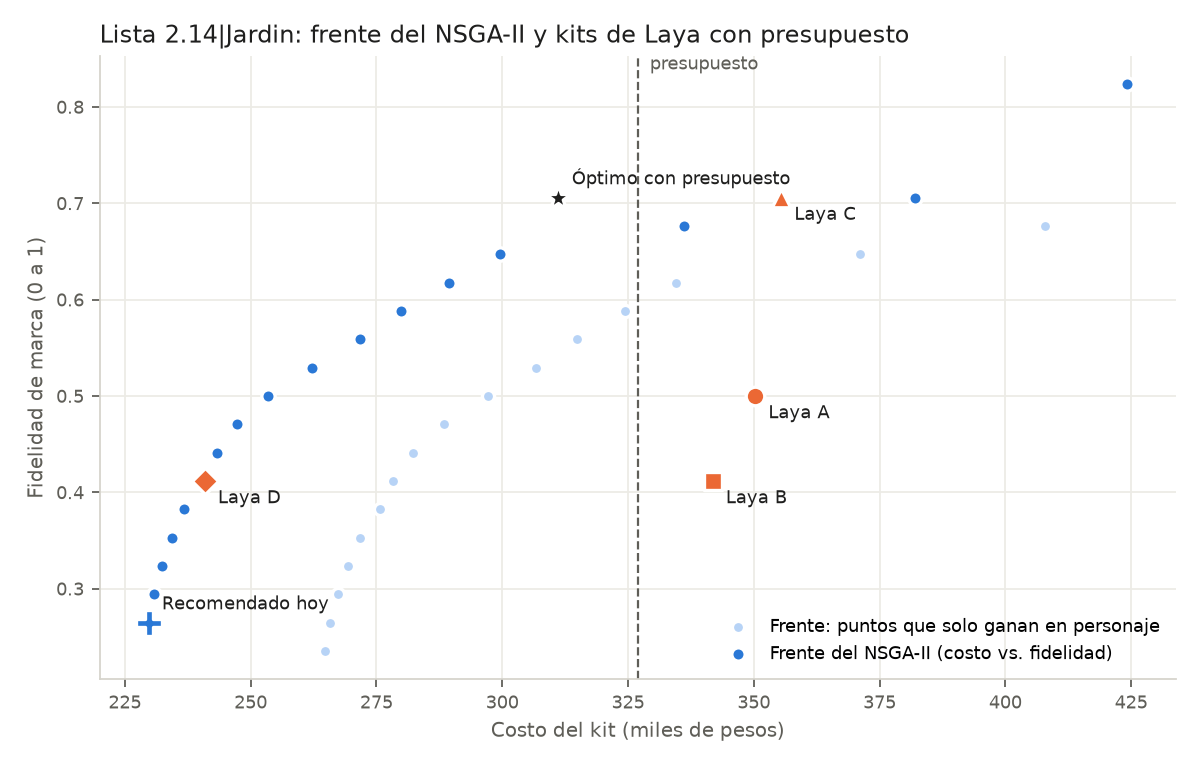
\includegraphics[width=0.88\textwidth]{../informes/benchmark-laya/fig_frente_2.14_Jardin.png}
\caption{Frente del NSGA-II proyectado en el plano costo-fidelidad para una
lista típica de 17 líneas. La cruz es el kit que se recomendaba en v3, el más
barato. Bajo la línea de presupuesto hay puntos del frente con fidelidad de
hasta 0,65, y el óptimo exacto (estrella, 0,70) queda por encima del frente,
lo que muestra que el frente es aproximado. Los puntos claros parecen
dominados en este plano, pero no lo están: ganan en el eje de personaje.
Los marcadores naranja son los kits del modelo de propósito general.}
\label{fig:frente-jardin}
\end{figure}

\subsection{Lectura de los resultados}

\begin{enumerate}
  \item \textbf{En los extremos, el NSGA-II es exacto, pero no es
        necesario.} Iguala el óptimo en el 100\,\% de los Premium y Fan y en el
        99,4\,\% de los Ahorrador promediando las cinco semillas. Es lo que
        predice el \cref{cor:extremos}: una regla línea por línea también es
        exacta. La regla simple fallaba el 20\,\% de los Ahorrador porque
        ordenaba por precio unitario (\cref{lem:precio-unitario}), y no por una
        limitación de las reglas voraces.
  \item \textbf{El aporte real del frente está en el compromiso.} Con
        presupuesto, el frente contenía kits que cabían y lograban el 94\,\%
        de la calidad posible, frente al 40\,\% del kit que se recomendaba. La
        diferencia no era de cómputo, porque el frente ya estaba calculado: la
        recomendación no lo usaba.
  \item \textbf{El frente es aproximado.} En el 68\,\% de las listas, la
        escalera de costo marginal dominaba algún punto del frente (en
        promedio el 5\,\% de sus puntos), lo que es coherente con el sesgo
        ordinal de los operadores (\cref{sec:opt-nsga}). Además, el óptimo
        exacto con presupuesto estaba por encima del mejor punto del frente en
        el 72\,\% de las listas.
  \item \textbf{Un modelo de decisión de propósito general no compite.} En sus
        modalidades línea por línea queda cerca del azar en Ahorrador y
        Premium: el sobrecosto medio es del 52\,\%, frente al 42,6\,\% del azar.
        Su prueba de cordura lo explica: acierta el 30\,\% de las preguntas
        «¿cuál es el más barato?» con entre 2 y 6 opciones, cuando el azar
        acierta el 31\,\%. Solo supera al azar cuando la respuesta consiste en
        encontrar una palabra (el personaje). Darle la lista completa lo
        empeora (en Fan baja del 92\,\% al 58\,\% de óptimos). Su mejor caso,
        juez entre kits (D), logra el 59\,\% de la calidad con presupuesto,
        pero ese resultado se debe sobre todo a los kits que se le entregan: un
        juez perfecto sobre los mismos kits llega al 93\,\%.
\end{enumerate}

\subsection{Efecto de las correcciones}

Las tres correcciones de la versión v4 (\cref{sec:opt-evolucion}) salieron
directamente de esta lectura. Repetida la evaluación con semilla 0 sobre las
mismas 174 listas:

\begin{table}[htbp]
\centering\small
\caption{Antes y después de las correcciones motivadas por la evaluación.}
\label{tab:antes-despues}
\begin{tabular}{@{}L{7.2cm}cc@{}}
\toprule
Métrica & v3 & v4 \\
\midrule
Regla simple: Ahorrador igual al óptimo & 80\,\% & 100\,\% \\
Listas en que la escalera domina algún punto del frente & 68\,\% & 0\,\% \\
Recomendado con presupuesto: calidad lograda & 40\,\% & igual al óptimo exacto \\
Recomendado con presupuesto: cabe en el tope & 100\,\% & 100\,\% \\
\bottomrule
\end{tabular}
\end{table}

La tercera fila requiere una precisión. Con presupuesto, la versión v4
recomienda el punto de mayor fidelidad del frente que cabe, y el frente ya
incluye los peldaños de la escalera. En estas instancias eso bastó para
alcanzar el óptimo exacto. El \cref{teo:mckp-poli} da una garantía que no
depende de la instancia: la programación dinámica alcanza el óptimo siempre.

\subsection{Reproducibilidad y tiempos}

Con cinco semillas, el NSGA-II entrega el mismo kit en el 94,5\,\% de las
listas en las que corre, y siempre en las que se enumeran. En las demás, el kit
cambia con la semilla; en el Ahorrador eso significa que en el 0,6\,\% de las
corridas el kit no es el más barato posible. Con la semilla fija que usa el
sistema, el resultado es determinista.

Los tiempos se midieron en 29 listas, en un proceso sin otras cargas, en una
CPU de 16 núcleos: 5,3~s de media, 6,3~s de mediana y 9,0~s de máximo para
producir \emph{todos} los kits de una lista. El modelo de propósito general en
una GPU portátil tarda entre 0,08 y 3,1~s por kit según la modalidad. Ninguno
de los dos tiempos limita el producto: son del mismo orden que leer una página
con el modelo multimodal.

\subsection{Limitaciones de la evaluación}

\begin{itemize}
  \item \textbf{Un hijo por lista.} La consolidación entre hermanos
        (\cref{sec:opt-lineas}) no entra en juego. Los hogares de varios hijos
        son el caso en que el acoplamiento podría aparecer.
  \item \textbf{Foto del catálogo a mitad de curaduría.} Con más candidatos
        por línea, el espacio crece y la calidad del frente puede cambiar.
  \item \textbf{Solo canal léxico.} Con el canal semántico, algunos renglones
        tendrían candidatos que aquí no tuvieron.
  \item \textbf{La fidelidad mide el nivel de marca}, no si el producto se
        parece a lo que escribió el colegio. Esa segunda dimensión es
        responsabilidad de la resolución y no se mide aquí.
  \item \textbf{Un solo tope de presupuesto.} El tope se fijó en la mitad del
        camino entre el Ahorrador y el Premium. Con otros topes, las cifras
        absolutas cambian.
\end{itemize}

% ============================================================================
\section{Evolución del núcleo}
\label{sec:evolucion}
% ============================================================================

Cada sección cerró con un recuadro de evolución propio. Esta sección los
ordena en el tiempo y extrae el patrón común. El sistema vigente reemplazó a
un conjunto de repositorios anteriores. No fue una reescritura: lo probado se
portó y lo que cambió fue el modelo de dominio, que era donde estaban los
defectos. Todas las fechas son de 2026.

\begin{figure}[htbp]
\centering
\begin{tikzpicture}[
  hito/.style={circle, fill=azul, inner sep=1.6pt},
  txt/.style={font=\footnotesize, align=left, text width=11.2cm, anchor=west},
  fecha/.style={font=\footnotesize\bfseries, anchor=east},
]
\draw[thick, gris] (0,0.5) -- (0,-9.6);
\foreach \y/\f/\t in {
  0/{21 sep}/{Monorrepositorio nuevo. Se portan el catálogo y el ciclo editorial; el modelo de dominio se rehace (cantidad y empaque separados, estados \textsc{SinMatch} y \textsc{HuecoCatálogo} distintos).},
  -1.5/{22 sep}/{Ciclo completo de punta a punta. Percepción todo-o-nada con rechazo por grados; normalización; emparejador léxico con cabeza anclada; optimizador \textbf{v1} (heurística declarada como andamio).},
  -3.4/{23 sep}/{Resolución híbrida: canal semántico con centroides de concepto y fusión por guardas. Optimizador \textbf{v2} (NSGA-II, variables reales y piso) y, el mismo día, \textbf{v3} (codificación entera, reparación por redondeo, población y generaciones escaladas, la biblioteca de optimización como dependencia obligatoria).},
  -5.6/{4 oct}/{\textbf{Evaluación} contra el óptimo exacto y un modelo de propósito general. Optimizador \textbf{v4} (costo de línea, siembra con la escalera, mejor marca que cabe) y \textbf{v5} (kits a pedido, A~tu~Medida, tope sin estirar). Curaduría de las 13 listas de un colegio: correcciones al emparejador caso por caso, concepto asignado que manda, tipo del concepto, reglas de segmentación y reintento en la percepción.},
  -8.6/{7 oct}/{Optimizador \textbf{v6}: herramientas por hijo. Vectores recalculados con huella nueva. Atributos del catálogo que filtran por lo que el colegio pide. Tras la formalización de este documento, optimizador \textbf{v7} (proyección sobre lo surtible) y coseno recortado en 0 en la resolución.}
}{
  \node[hito] at (0,\y) {};
  \node[fecha] at (-0.25,\y) {\f};
  \node[txt] at (0.3,\y) {\t};
}
\end{tikzpicture}
\caption{Línea de tiempo del núcleo algorítmico.}
\label{fig:linea-tiempo}
\end{figure}

\subsection{El patrón: defecto medido, cambio mínimo, efecto medido}

Casi todos los cambios del núcleo siguen el mismo ciclo:
\begin{enumerate}
  \item \textbf{Un defecto observable en un caso real}, no hipotético: un
        renglón concreto que se clasificaba mal, una lista concreta que se
        rechazaba, una cifra concreta de la evaluación.
  \item \textbf{Un diagnóstico de la causa}, distinto del síntoma. Por
        ejemplo, «lápices de colores» caía en esfero; el síntoma sugería
        alargar el prefijo comparado, pero la causa era comparar formas
        flexionadas, y la corrección fue singularizar.
  \item \textbf{El cambio más pequeño que elimina la causa}, fijado por una
        prueba con el caso original.
  \item \textbf{La verificación de que los vecinos no se mueven}: al cambiar
        un sinónimo o una regla, se vuelve a emparejar el corpus para comprobar
        que ningún otro renglón cambió de concepto.
\end{enumerate}

\Cref{tab:evolucion-resumen} resume los cambios de mayor efecto.

\begin{table}[htbp]
\centering\small
\caption{Cambios de mayor efecto en el núcleo.}
\label{tab:evolucion-resumen}
\begin{tabular}{@{}L{2.2cm}L{4.6cm}L{4.2cm}L{3.6cm}@{}}
\toprule
Etapa & Antes & Después & Evidencia \\
\midrule
Percepción & tope de 5 páginas que recortaba en silencio & todo o nada; guarda de 40 páginas; rechazo por grados & kits incompletos presentados como completos \\
Percepción & página que continúa marcada como incompleta & regla de continuación & 2 listas reales rechazadas \\
Percepción & un fallo de red invalidaba la lista & un reintento de transporte & página colgada 60~s, 6~s al reintentar \\
Normalización & cantidad y empaque en un número & $q$ y $\emp$ separados, $\techo{q/\emp}$ & «doce cajas» por doce lápices \\
Resolución & contención en cualquier posición & cabeza anclada & chaquiras $\to$ lápices de colores \\
Resolución & solo léxico & fusión con canal semántico & sinónimos no escritos («estuche») \\
Resolución & canal semántico inactivo en producción & una sola carga del índice & coseno siempre 0 \\
Catálogo & empaque 1 en todos los productos & regla «x$N$» salvo medida & la fórmula $\techo{q/\emp}$ no hacía nada \\
Catálogo & escaleras de nivel invertidas & nivelación por permutación & Ahorrador más caro que Premium \\
Optimización & NSGA-II separable que empataba con fuerza bruta & enumeración exacta + NSGA-II sembrado & pruebas del prototipo \\
Optimización & índice real con piso & índice entero con redondeo & SBX interpolaba etiquetas \\
Optimización & orden por precio unitario & orden por costo de línea & Ahorrador 80\,\% $\to$ 100\,\% \\
Optimización & recomendado con presupuesto = más barato & mejor marca que cabe, del frente & calidad 40\,\% $\to$ óptimo \\
Optimización & tres kits siempre & kits a pedido; A~tu~Medida & kits que nadie pedía \\
Optimización & herramientas cobradas por materia & una por hijo (máximo, no suma) & 43 renglones repetidos \\
Optimización & un candidato sin precio parecía gratis en el frente & proyección sobre los puntos de máxima disponibilidad & instancia de dos líneas (defecto latente) \\
Resolución & un coseno negativo podía restar & $\kappa$ recortado en 0 & propiedad «híbrido $\geq$ léxico» \\
\bottomrule
\end{tabular}
\end{table}

\subsection{Lo que se decidió no cambiar}

La evolución también se ve en lo que se conservó a propósito. La aritmética
de unidades, la regla de que lo informativo no se cobra y la separación entre
\textsc{SinMatch} y \textsc{HuecoCatálogo} se definieron en la primera
versión y no cambiaron en ninguna de las siguientes, porque no dependen del
algoritmo. El optimizador se reemplazó tres veces sin tocarlas. Esa
estabilidad es el resultado del principio «separar decidir de presentar»
(\cref{sec:principios}).

% ============================================================================
\section{Discusión, limitaciones y trabajo futuro}
\label{sec:discusion}
% ============================================================================

\subsection{Síntesis}

El núcleo de Tukit encadena tres familias de algoritmos de naturaleza muy
distinta: la lectura con un modelo multimodal, envuelta en reglas
deterministas de aceptación; la clasificación por reglas léxicas con un canal
semántico subordinado; y la optimización combinatoria multiobjetivo. Lo que
las une es una misma postura frente al error. Cada etapa tiene una salida
explícita para «no sé» o «no tengo», y en cada etapa el error barato
(rechazar, abstenerse, mandar a revisión) se prefiere al error caro (aceptar
una lista truncada, ofrecer un producto equivocado, recomendar un kit que no
cabe).

El resultado analítico más importante de este documento es estructural
(\cref{sec:opt-estructura}). Con la formulación vigente, los objetivos son
separables por línea, los extremos se resuelven de forma voraz y exacta, el
compromiso con presupuesto es una mochila de elección múltiple con valores
pequeños y, por lo tanto, polinomial, y el frente completo de cuatro objetivos
se calcula exactamente en $O(n^4k)$. La evaluación empírica es coherente con
ese análisis: el NSGA-II es exacto en los extremos, donde no hace falta, y
aproximado en el frente, donde hay una alternativa exacta.

\subsection{Limitaciones}

\begin{itemize}
  \item \textbf{Sin acoplamiento en el objetivo.} El costo no ve la
        consolidación entre hermanos ni la agrupación de herramientas, que se
        aplican después de elegir, ni un costo por tienda. El optimizador
        resuelve un problema más simple que el real en hogares de varios hijos.
  \item \textbf{Frente aproximado.} El NSGA-II con operadores ordinales sobre
        una variable nominal no garantiza el frente exacto, aunque la siembra
        garantiza no quedar por debajo de la heurística ni de la escalera
        (\cref{prop:siembra}).
  \item \textbf{Umbral de rescate y revisión:} un rescate con coseno de al
        menos 0,93 se acepta sin revisión humana, contra la intención declarada
        del piso de rescate. Su impacto medido es bajo (\cref{tab:cosenos}).
  \item \textbf{Recuperación limitada a la estructura léxica.} Sin el grafo de
        sustituibilidad y sin reordenador, el \emph{recall} de la resolución
        está acotado por los sinónimos escritos y por el rescate semántico.
  \item \textbf{Pesos por omisión} distintos de los medidos en la encuesta
        (\cref{sec:opt-recomendar}).
  \item \textbf{Percepción secuencial}: el tiempo de la primera lectura crece
        linealmente con el número de páginas.
\end{itemize}

\subsection{Trabajo futuro, en orden de impacto}

\begin{enumerate}
  \item \textbf{Frente exacto por programación dinámica.} Reemplazar el
        NSGA-II, o complementarlo como verificación, con la recurrencia del
        \cref{teo:frente-poli}. Para una lista típica son unos $10^4$ estados
        frente a unas $10^7$ operaciones del NSGA-II, y el frente pasaría a ser
        exacto y determinista sin depender de una semilla.
  \item \textbf{Llevar el acoplamiento al objetivo}, si se quiere que el
        optimizador resuelva el problema del hogar completo: la consolidación
        dentro de $f_1$ ---el costo de un producto depende de la demanda
        agregada de los hermanos que lo comparten--- y, eventualmente, un costo
        fijo por tienda. Con ese acoplamiento, la \cref{prop:separable} deja de
        valer y una metaheurística vuelve a estar justificada. En ese caso
        convendría cambiar SBX y PM por operadores categóricos (cruce uniforme
        y mutación por reemplazo aleatorio del índice) y medir con
        hipervolumen \cite{zitzler1999} contra el frente exacto en instancias
        pequeñas. El diseño original preveía también una prueba de falsación:
        sin acoplamiento, la heurística y el NSGA-II deben empatar en
        hipervolumen. Si empatan, queda demostrado que el acoplamiento es la
        contribución.
  \item \textbf{Rescate siempre revisado}: que la respuesta del emparejamiento
        indique que el concepto vino de un rescate semántico y que ese renglón
        vaya a revisión sin importar su puntaje. Requiere agregar un campo al
        contrato entre servicios.
  \item \textbf{Grafo de sustituibilidad y reordenador}, con una evaluación
        que separe «no lo tenemos» de «no lo encontramos» y mida el
        \emph{recall} antes que el ordenamiento.
  \item \textbf{Calibrar} $\tau$ y los pesos de recomendación con datos de uso:
        el umbral de autoaceptación contra las correcciones de los revisores y
        los pesos contra la encuesta.
  \item \textbf{Paralelizar la percepción} por página respetando la cuota del
        proveedor.
  \item \textbf{Evaluar hogares de varios hijos}, que es donde la
        consolidación puede cambiar qué kit es mejor.
\end{enumerate}

\subsection{Conclusión}

Los algoritmos del núcleo son, en su mayoría, sencillos: listas de
decisión, distancias de edición acotadas, coeficientes de Jaccard, centroides,
ordenamientos y programación dinámica. Su valor está en la precisión con que
se delimita cada problema ---qué se decide, con qué información y qué se hace
cuando no se puede decidir---, en que cada regla se justifica con un caso real
y en que las propiedades importantes (no truncar, no fabricar, no restar, no
encarecer, no quedar por debajo de la semilla) se pueden enunciar y demostrar.
El componente más sofisticado, el NSGA-II, es también el que este análisis
señala como el más fácil de reemplazar por algo exacto, mientras la
formulación siga sin acoplamiento entre líneas.


\appendix
% ============================================================================
\section{Parámetros numéricos}
\label{ap:parametros}
% ============================================================================

Todas las constantes del núcleo, con su valor y la razón que lo fija. Las
marcadas con $\ast$ se leen del entorno y se pueden cambiar sin modificar el
código.

\begin{table}[H]
\centering\small
\begin{tabular}{@{}L{3.5cm}L{3.9cm}L{7.6cm}@{}}
\toprule
Parámetro & Valor & Justificación \\
\midrule
\multicolumn{3}{@{}l}{\emph{Percepción}}\\
Tope de páginas & 40 & Justo por encima del PDF más largo del corpus (39 páginas). \\
Resolución de rasterizado & 150 DPI & Basta para leer una tabla como tabla; más resolución encarece la llamada sin ganancia. \\
Temperatura & 0 & Decodificación voraz: menor variabilidad entre lecturas. \\
Tiempo límite por llamada & 40 s & Una página típica tarda unos 5 s; 40 s ya es una llamada colgada. \\
Reintentos & 1 (solo de transporte) & Ante 429, 5xx o falta de respuesta; no ante 403 ni respuesta mal formada. \\
Espera entre intentos & 3 s & Peor caso por página: 83 s. \\
Modelo multimodal$^\ast$ & configurable & Puerto con una sola implementación; cambiarlo no toca las reglas. \\
\midrule
\multicolumn{3}{@{}l}{\emph{Resolución}}\\
Longitud mínima para corregir & 5 & Tokens más cortos tienen demasiados vecinos a distancia 1. \\
Distancia máxima & 1 (OSA) & Un error de dedo; la transposición cuenta como uno. \\
Prefijo de «misma cosa» & 5 caracteres & Sobre singulares; prefijos más cortos emparejan «lápida». \\
Palabras de la consulta & 6 & Los adjetivos discriminan; más palabras empeoran la búsqueda. \\
$\alpha$ (piso del ancla) & 0,6 & Acertar la cabeza basta para reconocer, no para autoaceptar. \\
$\beta$ (peso del Jaccard) & 0,4 & Con $\alpha$, el ancla perfecta vale 1. \\
$\gamma$ (aporte del coseno) & 0,15 & Pequeño: desempata, no decide. \\
$\theta$ (umbral de rescate) & 0,86 & Separa «la misma cosa dicha de otro modo» de «un tema parecido». \\
$\phi$ (piso del rescate) & 0,55 & Apenas sobre el umbral de reconocimiento. \\
Umbral de reconocimiento & 0,5 & Por debajo, \textsc{SinMatch}. \\
$\tau$ (autoaceptación)$^\ast$ & 0,75 & Por debajo, revisión humana; se puede subir cuando el catálogo esté más completo. \\
Opciones por renglón & $\leq3$ & Una por nivel; acota $\card{\Esp}\leq3^n$. \\
Dimensión de los vectores & 1024 & Fijada por la columna y el índice de la base. \\
Lote de \emph{embeddings} & 100 textos & Una petición por lote; evita cuerpos gigantes. \\
\bottomrule
\end{tabular}
\end{table}

\begin{table}[H]
\centering\small
\begin{tabular}{@{}L{3.5cm}L{3.9cm}L{7.6cm}@{}}
\toprule
Parámetro & Valor & Justificación \\
\midrule
\multicolumn{3}{@{}l}{\emph{Catálogo}}\\
Rango de precio en tiendas & \$1.000 -- \$400.000 & Descarta accesorios sueltos y lotes institucionales. \\
Propuestas por renglón & 3 (cuantiles 1/6, 1/2, 5/6) & Quien revisa compara pocas; se evitan los extremos. \\
Longitudes válidas de EAN & 8, 12, 13 & Las de 12 se normalizan a 13. \\
\midrule
\multicolumn{3}{@{}l}{\emph{Optimización}}\\
Límite de enumeración & $4096=2^{12}$ & Por debajo, el frente exacto cuesta milisegundos. \\
Población $N$ & $\min(200,\max(40,12n))$, par & Escala con las líneas decidibles. \\
Generaciones $G$ & $\min(120,\max(30,$ $20\log_{10}\card{\Esp}))$ & Escala con el logaritmo del espacio. \\
SBX & $p_c=0{,}9$, $\eta_c=15$ & Valores estándar \cite{deb1995sbx}. \\
PM & $p=1$ por individuo; $1/n$ por variable; $\eta_m=20$ & Valores estándar \cite{deb1996pm}. \\
Semilla & 0 & Reproducibilidad byte a byte. \\
Umbral de sobreprecio para Premium & $\sigma\geq0{,}10$ & Encuesta: 42 de 60 pagan como máximo un 5\,\% más. \\
Tope sin presupuesto (A~tu~Medida) & mitad del camino & Entre el total del Ahorrador y el del Premium. \\
\bottomrule
\end{tabular}
\end{table}

% ============================================================================
\section{Correspondencia con la implementación}
\label{ap:codigo}
% ============================================================================

Para quien quiera contrastar el documento con el código, esta tabla indica
dónde vive cada algoritmo. Las rutas son relativas a \cod{servicios/}.

\begin{table}[H]
\centering\footnotesize
\begin{tabular}{@{}L{5.4cm}L{9.6cm}@{}}
\toprule
Algoritmo & Módulo y función \\
\midrule
Percepción (\cref{alg:percibir}) & \cod{inteligencia/.../percepcion.py}: \cod{percibir}, \cod{normalizar\_grado} \\
Rasterizado & \cod{inteligencia/.../paginas.py}: \cod{renderizar} \\
Lectura estructurada y reintento & \cod{inteligencia/.../gemini.py}: \cod{pedir\_pagina}, \cod{\_llamar} \\
Normalización & \cod{inteligencia/.../parseo.py}: \cod{parsear\_renglon}; \cod{dominio/pipeline.py}: \cod{\_normalizar} \\
Corrección ortográfica & \cod{catalogo/.../transcripcion.py}: \cod{corregir}, \cod{\_distancia}, \cod{\_unica} \\
Cabeza, singular, Jaccard & \cod{catalogo/.../descubrir.py}: \cod{cabeza}, \cod{singular}, \cod{\_parecido} \\
Clasificación (\cref{alg:clasificar}) & \cod{catalogo/.../descubrir.py}: \cod{clasificar} \\
Vectores y centroides & \cod{catalogo/.../embeddings.py}: \cod{coseno}, \cod{promedio}, \cod{texto\_de\_producto} \\
Emparejamiento (\cref{alg:emparejar}) & \cod{catalogo/.../consulta.py}: \cod{emparejar}, \cod{cargar\_indice} \\
Atributos y empaque & \cod{catalogo/.../enriquecer.py}: \cod{extraer\_atributos}, \cod{extraer\_empaque} \\
Nivelación & \cod{catalogo/.../nivelar.py}: \cod{reacomodar} \\
Búsqueda en tiendas & \cod{catalogo/.../descubrir.py}: \cod{buscar\_candidatos} \\
Estado de resolución & \cod{inteligencia/.../dominio/pipeline.py}: \cod{estado\_desde\_emparejamiento} \\
Frente exacto (\cref{alg:frente-exacto}) & \cod{inteligencia/.../optimizador.py}: \cod{\_frente\_exacto}, \cod{\_no\_dominadas} \\
NSGA-II (\cref{alg:nsga2}) & \cod{inteligencia/.../optimizador.py}: \cod{\_frente\_nsga}, \cod{\_poblacion\_inicial} \\
Escalera (\cref{alg:escalera}) & \cod{inteligencia/.../optimizador.py}: \cod{\_escalera\_costo\_marginal} \\
Proyección y heurística & \cod{inteligencia/.../optimizador.py}: \cod{\_proyectar}, \cod{\_surtibles}, \cod{elegir\_por\_perfil} \\
Herramientas y consolidación & \cod{inteligencia/.../optimizador.py}: \cod{juntar\_herramientas}, \cod{consolidar} \\
A tu Medida y recomendación & \cod{inteligencia/.../optimizador.py}: \cod{\_armar\_a\_tu\_medida}, \cod{recomendar} \\
Personaje & \cod{inteligencia/.../dominio/pipeline.py}: \cod{inyectar\_personaje\_fan}; \cod{optimizador.py}: \cod{anclar\_personaje} \\
Orquestación (\cref{alg:armar}) & \cod{inteligencia/.../optimizador.py}: \cod{armar\_los\_tres}; \cod{trabajos.py}: \cod{procesar} \\
\bottomrule
\end{tabular}
\end{table}


% ============================================================================
%  Referencias
% ============================================================================
\begin{thebibliography}{99}
\addcontentsline{toc}{section}{Referencias}

\bibitem{blank2020pymoo}
J.~Blank y K.~Deb.
\newblock pymoo: Multi-objective optimization in Python.
\newblock \emph{IEEE Access}, 8:89497--89509, 2020.

\bibitem{cormack2009rrf}
G.~V. Cormack, C.~L.~A. Clarke y S.~Büttcher.
\newblock Reciprocal rank fusion outperforms Condorcet and individual rank
  learning methods.
\newblock En \emph{Proceedings of the 32nd International ACM SIGIR Conference},
  pp.~758--759, 2009.

\bibitem{cormen2009}
T.~H. Cormen, C.~E. Leiserson, R.~L. Rivest y C.~Stein.
\newblock \emph{Introduction to Algorithms}, 3.\textsuperscript{a} ed.
\newblock MIT Press, 2009.

\bibitem{damerau1964}
F.~J. Damerau.
\newblock A technique for computer detection and correction of spelling errors.
\newblock \emph{Communications of the ACM}, 7(3):171--176, 1964.

\bibitem{deb1995sbx}
K.~Deb y R.~B. Agrawal.
\newblock Simulated binary crossover for continuous search space.
\newblock \emph{Complex Systems}, 9(2):115--148, 1995.

\bibitem{deb1996pm}
K.~Deb y M.~Goyal.
\newblock A combined genetic adaptive search (GeneAS) for engineering design.
\newblock \emph{Computer Science and Informatics}, 26(4):30--45, 1996.

\bibitem{deb2002nsga2}
K.~Deb, A.~Pratap, S.~Agarwal y T.~Meyarivan.
\newblock A fast and elitist multiobjective genetic algorithm: NSGA-II.
\newblock \emph{IEEE Transactions on Evolutionary Computation}, 6(2):182--197,
  2002.

\bibitem{ehrgott2005}
M.~Ehrgott.
\newblock \emph{Multicriteria Optimization}, 2.\textsuperscript{a} ed.
\newblock Springer, 2005.

\bibitem{garey1979}
M.~R. Garey y D.~S. Johnson.
\newblock \emph{Computers and Intractability: A Guide to the Theory of
  NP-Completeness}.
\newblock W.~H. Freeman, 1979.

\bibitem{jaccard1912}
P.~Jaccard.
\newblock The distribution of the flora in the alpine zone.
\newblock \emph{New Phytologist}, 11(2):37--50, 1912.

\bibitem{keeney1976}
R.~L. Keeney y H.~Raiffa.
\newblock \emph{Decisions with Multiple Objectives: Preferences and Value
  Tradeoffs}.
\newblock Wiley, 1976.

\bibitem{kellerer2004}
H.~Kellerer, U.~Pferschy y D.~Pisinger.
\newblock \emph{Knapsack Problems}.
\newblock Springer, 2004.

\bibitem{lee2025gemini}
J.~Lee et al.
\newblock Gemini Embedding: Generalizable embeddings from Gemini.
\newblock \emph{arXiv:2503.07891}, 2025.

\bibitem{levenshtein1966}
V.~I. Levenshtein.
\newblock Binary codes capable of correcting deletions, insertions, and
  reversals.
\newblock \emph{Soviet Physics Doklady}, 10(8):707--710, 1966.

\bibitem{malkov2018hnsw}
Y.~A. Malkov y D.~A. Yashunin.
\newblock Efficient and robust approximate nearest neighbor search using
  hierarchical navigable small world graphs.
\newblock \emph{IEEE Transactions on Pattern Analysis and Machine
  Intelligence}, 42(4):824--836, 2020.

\bibitem{miettinen1999}
K.~Miettinen.
\newblock \emph{Nonlinear Multiobjective Optimization}.
\newblock Kluwer, 1999.

\bibitem{rivest1987decision}
R.~L. Rivest.
\newblock Learning decision lists.
\newblock \emph{Machine Learning}, 2(3):229--246, 1987.

\bibitem{sinha1979mckp}
P.~Sinha y A.~A. Zoltners.
\newblock The multiple-choice knapsack problem.
\newblock \emph{Operations Research}, 27(3):503--515, 1979.

\bibitem{wagner1974}
R.~A. Wagner y M.~J. Fischer.
\newblock The string-to-string correction problem.
\newblock \emph{Journal of the ACM}, 21(1):168--173, 1974.

\bibitem{zitzler1999}
E.~Zitzler y L.~Thiele.
\newblock Multiobjective evolutionary algorithms: A comparative case study and
  the strength Pareto approach.
\newblock \emph{IEEE Transactions on Evolutionary Computation}, 3(4):257--271,
  1999.

\end{thebibliography}


\end{document}
